基于色散相位与变量投影的外延层厚度反演及多光束影响分析

摘要

红外反射谱中的干涉周期携带外延层厚度信息，但折射率色散、慢变背景与高阶反射会影响直接读峰测厚。本文以``相位决定厚度、幅度用于诊断''为主线，建立两光束物理模型，再将实测反演化为带线性子问题的一维厚度搜索。

针对问题1，依据Snell定律与Fresnel关系推导斜入射光程差，引入\textbf{色散相位函数}校正极值间隔。厚度真值为10
μm的合成实验中，相位法与全谱拟合分别得到约 \textbf{10.002 μm} 和
\textbf{10.000
μm}；常数折射率近似存在约4\%的系统偏差，只作为对照。针对问题2，以\textbf{变量投影}分离慢变基线和干涉项，碳化硅两角共享厚度为
\textbf{7.2158 μm}，独立估计的相对差为 \textbf{0.165\%}。F检验给出
\(p=0.022\)，说明统计显著差异与工程容差内的一致性必须分别报告。针对问题3，利用Airy多光束模型分析高阶反射的形成条件，硅共享厚度为
\textbf{3.4477 μm}，两角相对差为
\textbf{0.130\%}；物理基线下多光束残差最大改善约0.11\%，当前谱段无需增加显著多光束修正。

扰动与消融结果支持采用相位信息测厚，但结果仍受材料色散依据、背景建模和周期候选接近程度约束。本文明确区分合成恢复精度、实测一致性和条件置信区间，不把内部一致性当作外部真值验证。

关键词

外延层厚度；红外干涉；折射率色散；变量投影；多光束干涉

问题重述

题目要求根据晶圆红外反射谱确定外延层厚度。问题1在界面仅发生一次反射、透射的条件下建立两光束模型；问题2利用同一碳化硅晶圆在10°和15°入射角下的测量谱，设计反演算法并评价可靠性；问题3进一步分析多次反射形成的多光束干涉，用硅晶圆的两角数据判断是否需要修正，并返回检验碳化硅结论。四份附件均以波数为第一列、反射率百分数为第二列。

测量对象不是一个独立的频率常数：折射率随波长变化，衬底与外延层的掺杂差异影响界面反射，而背景与噪声可能制造并非真实干涉周期的极值。因此，本文不仅给出厚度数值，还说明这些数值依赖哪些观测信息、适用哪些物理条件，以及有哪些不能消除的不确定性。

问题分析与总体流程

红外干涉测厚、材料光学常数和多层反射构成本文的方法背景。早期测厚研究与相关测试方法说明该问题具有明确的光学基础
{[}1{]}、{[}2{]}、{[}3{]}、{[}4{]}、{[}5{]}；反射、折射与干涉公式沿用光学教材的约定
{[}6{]}、{[}7{]}。本文的具体参数和数值仍以已完成的实验记录为准，不把文献题名中的性能结论移用于本数据。

总体流程为：统一单位和有效谱段，建立斜入射相位函数，用合成场景验证公式与求解的一致性，再将实测谱分解为慢变背景和振荡项；固定候选厚度时解线性最小二乘，扫描厚度得到共同估计和独立角度估计；最后比较扰动、消融与Airy修正，形成附条件结论。

两光束模型提供可解释的相位结构；变量投影承担实测背景不确定性；Airy模型用于检验高阶反射是否重要。三者不是互相替代的``更复杂算法''，而是回答不同层次的问题。

模型假设

\begin{enumerate}
\def\labelenumi{\arabic{enumi}.}
\tightlist
\item
  在选定透明谱段内，外延层及衬底折射率可按实数近似处理；强吸收区不纳入同一无吸收模型。
\item
  两界面在照射区域近似平行，入射角已知；共享厚度表示两次测量对应同一晶圆的近似共同厚度，角度间差异另作诊断。
\item
  同型相邻极值相差一个完整干涉周期。反射相位跃变影响峰谷标签，但在一致的同型间隔中抵消。
\item
  色散模型只在有材料依据的谱段内使用。慢变基线和包络可由预先固定的低阶多项式近似，不允许任意高阶趋势吸收干涉周期。
\item
  主反演厚度由相位积累率确定；从幅度辨识的衬底折射率只作弱辨识诊断，不作为已精确标定的材料常数。
\end{enumerate}

这些假设并非对整个红外谱无条件成立。其有效性由谱段选择、两角对照和扰动实验限定；SiC和硅使用各自的材料色散关系。

符号说明

主要符号与单位约定

\begin{longtable}[]{@{}lll@{}}
\toprule\noalign{}
符号 & 含义 & 单位 \\
\midrule\noalign{}
\endhead
\bottomrule\noalign{}
\endlastfoot
\(t\) & 外延层厚度 & μm \\
\(\nu\) & 真空波数 & cm⁻¹ \\
\(\lambda\) & 真空波长，\(\lambda=10^4/\nu\) & μm \\
\(\theta,\theta'\) & 空气侧入射角、层内折射角 & °，计算时转弧度 \\
\(n,n_{\mathrm{sub}}\) & 外延层、衬底折射率 & 无量纲 \\
\(\delta,g\) & 往返相位差、色散相位函数 & rad、cm⁻¹ \\
\(R_{01},R_{12}\) & 两界面强度反射率 & 无量纲 \\
\(B,C,S\) & 慢变基线、余弦和正弦包络 & 无量纲 \\
\(J(t)\) & 两角加权残差平方和 & 无量纲 \\
\(\bar R,\mathcal F\) & 界面反射率几何平均、精细度参数 & 无量纲 \\
\end{longtable}

数据说明与预处理

输入数据的材料与测量条件

\begin{longtable}[]{@{}llll@{}}
\toprule\noalign{}
附件 & 材料 & 入射角 & 本文用途 \\
\midrule\noalign{}
\endhead
\bottomrule\noalign{}
\endlastfoot
1 & 碳化硅 & 10° & 厚度联合反演与角度对照 \\
2 & 碳化硅 & 15° & 厚度联合反演与异常点诊断 \\
3 & 硅 & 10° & 厚度反演与多光束判定 \\
4 & 硅 & 15° & 共享厚度与独立角度对照 \\
\end{longtable}

反射率百分数除以100转换为无量纲量；按波数统一排列，再执行既定有效谱段筛选。两种材料的主反演均采用
\([2000,4000]\ \mathrm{cm}^{-1}\)。SiC近Reststrahlen区的强吸收不能沿用实折射率模型，且
\(\lambda>5\ \mu\mathrm m\)
的色散依据不足；硅则避开多声子吸收显著的低波数区域。

反射率大于100\%的记录不被改成物理范围内的假数据；原分析采用降权、剔除与保留策略作比较，异常点降权权重为0.05。附件2的当前文件与最初输入清单存在字节一致性差异，现有结果只能对应其计算时记录的输入与条件，不能宣称已经完成跨副本复现。本文不替换附件、不重新生成计算结果。

问题1 两光束测厚模型与合成验证

问题1 问题分析与几何光程差

一束光在空气---外延层界面直接反射，另一束光进入外延层，在衬底界面反射后返回空气。利用Snell定律消去折射角，往返相位写成

\[n_{\mathrm{air}}\sin\theta=n(\nu)\sin\theta',\qquad
\Delta=2nt\cos\theta'=2t\sqrt{n(\nu)^2-\sin^2\theta},\]

其中取
\(n_{\mathrm{air}}=1\)。厚度以μm、波数以cm⁻¹计时，必须保留单位换算因子：

\[\delta(\nu)=4\pi\times10^{-4}\,t\,n(\nu)\nu\cos\theta'. \]

若遗漏 \(10^{-4}\)，即使数值程序收敛，也不具有正确的物理量纲。

问题1 反射率与色散修正

以 \(R_{01}\)、\(R_{12}\)
表示由Fresnel关系得到的界面强度反射率，两光束近似为

\[R_{2b}=R_{01}+(1-R_{01})^2R_{12}
+2(1-R_{01})\sqrt{R_{01}R_{12}}\cos\delta.\]

反射相位的常数跃变按界面约定处理；未指定偏振时使用两种偏振结果的平均。界面反射率不能替代材料色散，后者会直接影响相位积累
{[}8{]}、{[}9{]}、{[}10{]}、{[}11{]}。

定义
\(g(\nu)=n(\nu)\nu\cos\theta'(\nu)\)。在振幅缓变且峰谷可可靠定位的条件下，同型相邻极值满足

\[\Delta\delta=2\pi,\qquad
t=\frac{10^4}{2\,[g(\nu_{m+2})-g(\nu_m)]}.\]

当折射率近似常数时，该式退化为

\[t\approx\frac{10^4}{2n\cos\theta'\,\Delta\nu}.\]

这里的间隔是峰---峰或谷---谷间隔，不是相邻峰谷之间的半周期。涉及厚度与折射率共同估计的干涉条纹方法可作为背景参考
{[}18{]}，但本文不据此忽略实测峰检出的噪声问题。

问题1 求解与结果解释

合成场景设置
\(t_{\mathrm{true}}=10\ \mu\mathrm m\)、\(n_{\mathrm{sub}}=3.0\)，分别比较常数折射率间隔法、色散化相位法和全谱非线性最小二乘。相位法约10.002
μm，全谱拟合约10.000
μm；常数折射率方案产生约4\%的系统偏差。合成真值已知，所以这些结果可以用来检验反演一致性；实测晶圆没有独立真值，不能照搬这一精度措辞。

\pandocbounded{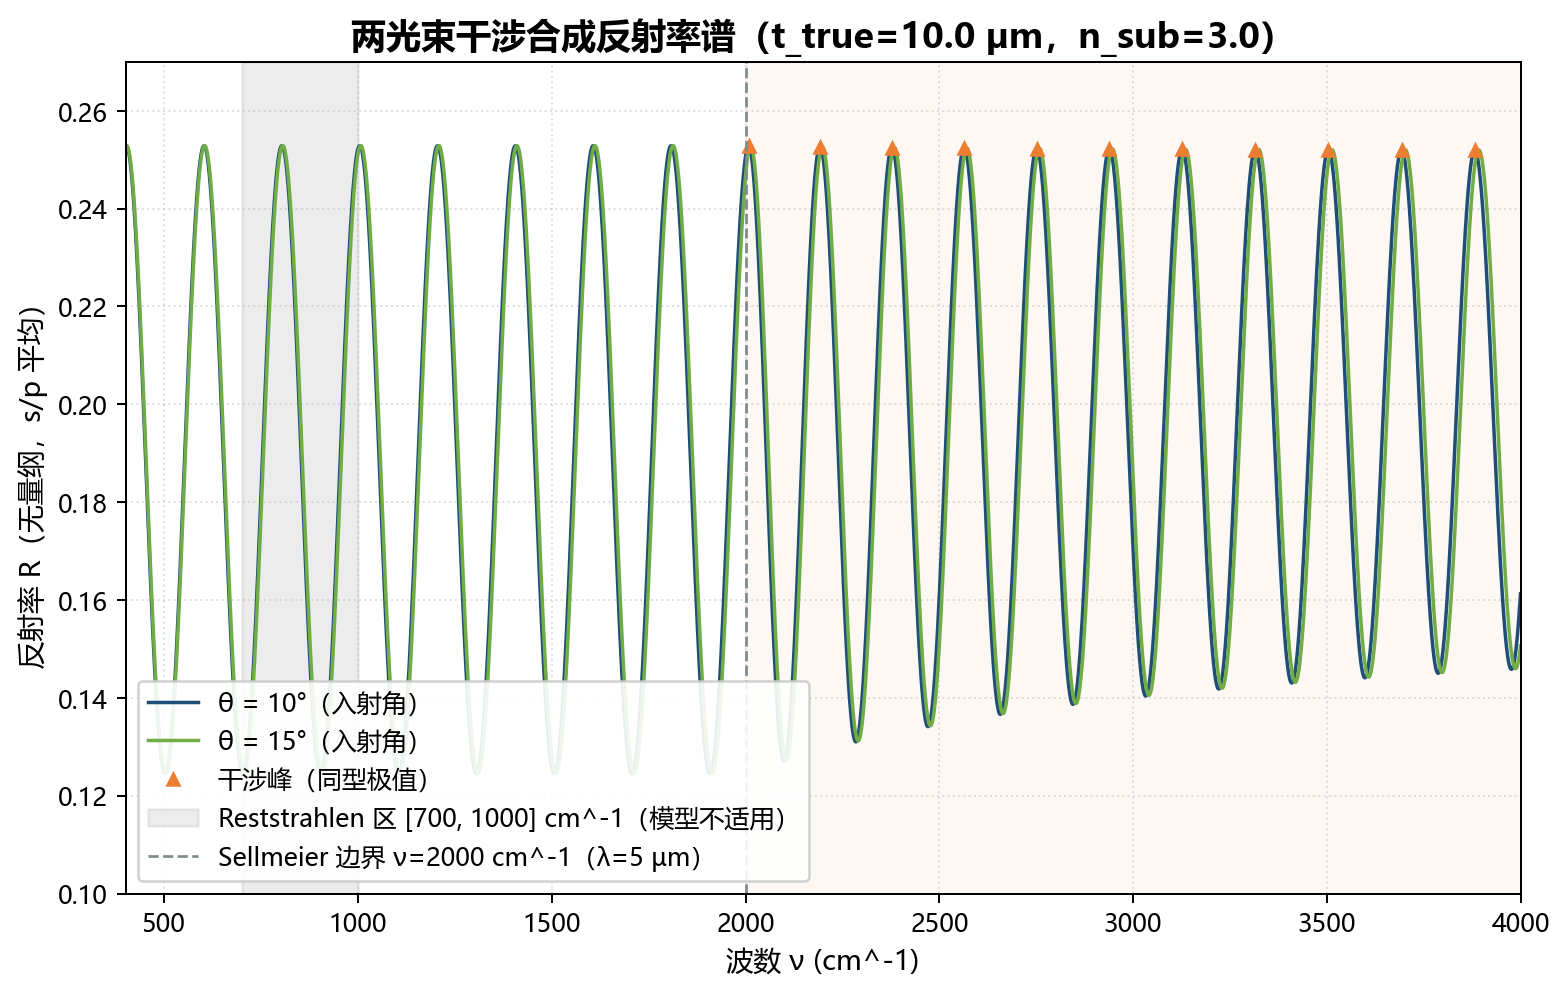
\includegraphics[keepaspectratio,alt={合成两光束反射率谱与极值位置}]{problems/2025-cumcm-b/prob01/versions/assumption_v001/figures/prob01_fig_reflectance_spectrum_1d4fb899d1.png}}

合成两光束反射率谱与极值位置

图1 给出厚度真值为10
μm的合成光谱。两种角度的条纹位置随折射角发生系统变化；合成数据用于检验公式与求解程序，不能视为实际晶圆测量。

\pandocbounded{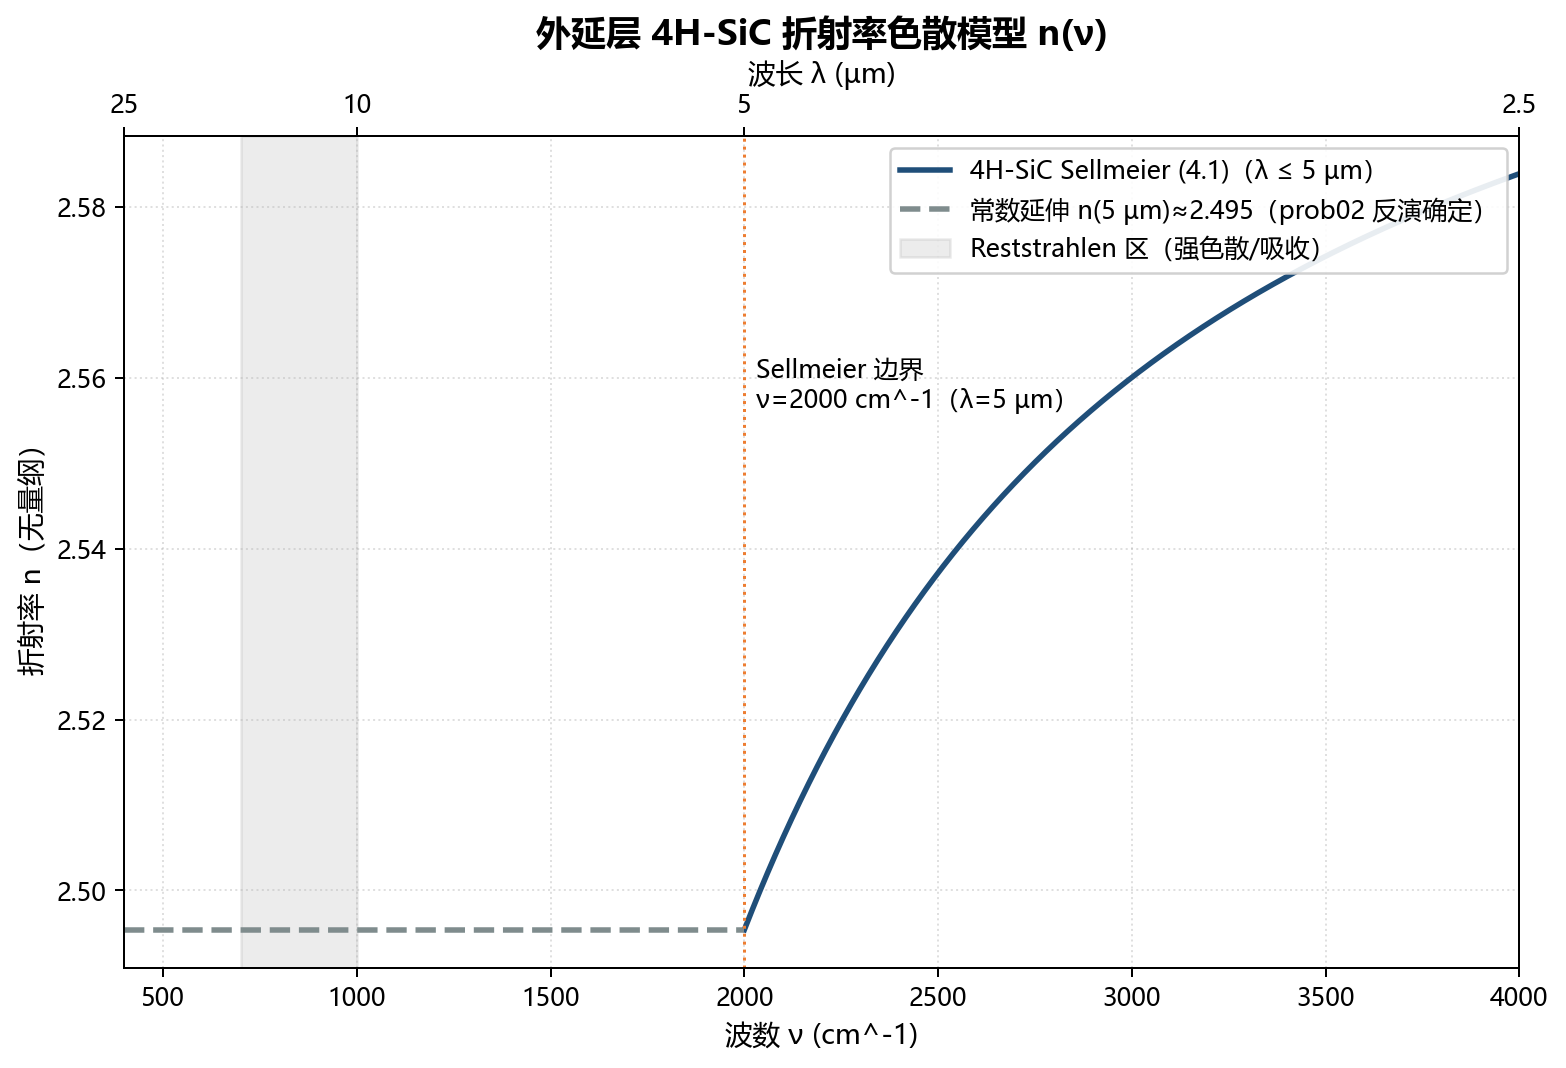
\includegraphics[keepaspectratio,alt={碳化硅折射率的波数依赖与适用谱段}]{problems/2025-cumcm-b/prob01/versions/assumption_v001/figures/prob01_fig_dispersion_curve_d85564d2fc.png}}

碳化硅折射率的波数依赖与适用谱段

图2
显示色散曲线及其适用边界。不能把谱段外的常数延伸当作文献已证实的材料规律；实测反演因此限于色散信息有依据的波段。

\pandocbounded{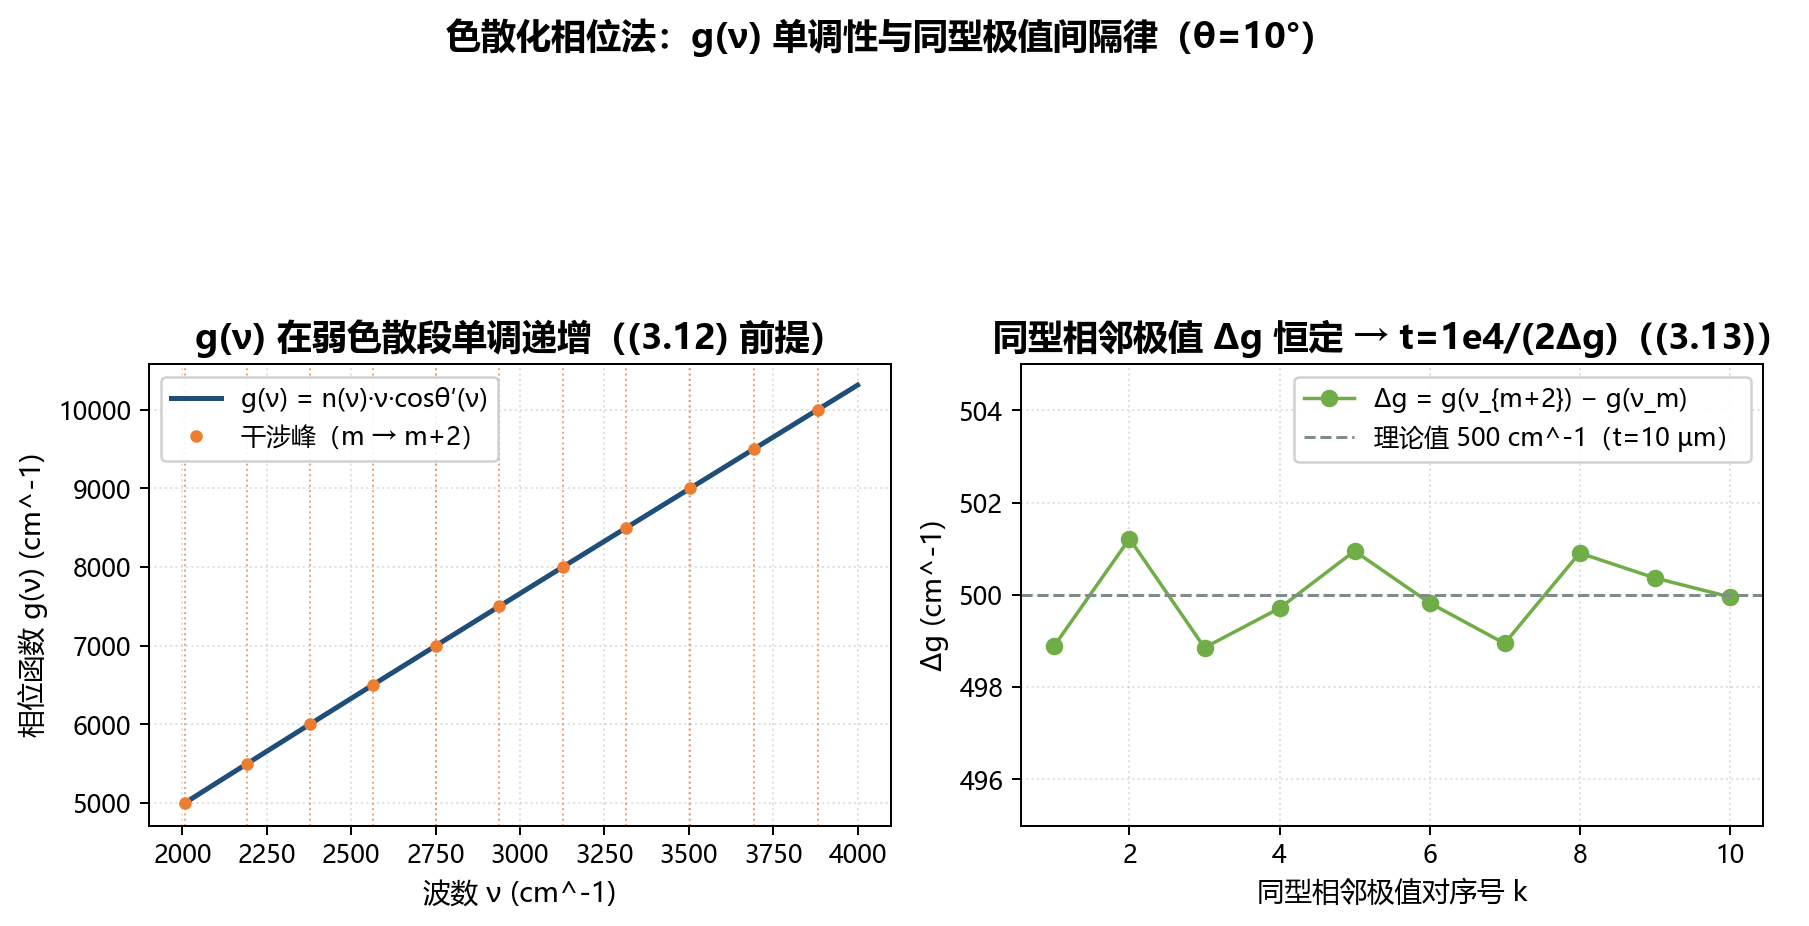
\includegraphics[keepaspectratio,alt={相位函数与同型极值间隔}]{problems/2025-cumcm-b/prob01/versions/assumption_v001/figures/prob01_fig_phase_function_gap_459c486470.png}}

相位函数与同型极值间隔

图3
展示从波数到相位函数坐标的变换。同型峰之间近似恒定的相位函数间隔对应固定厚度，比忽略色散的波数间隔更接近模型前提。

\pandocbounded{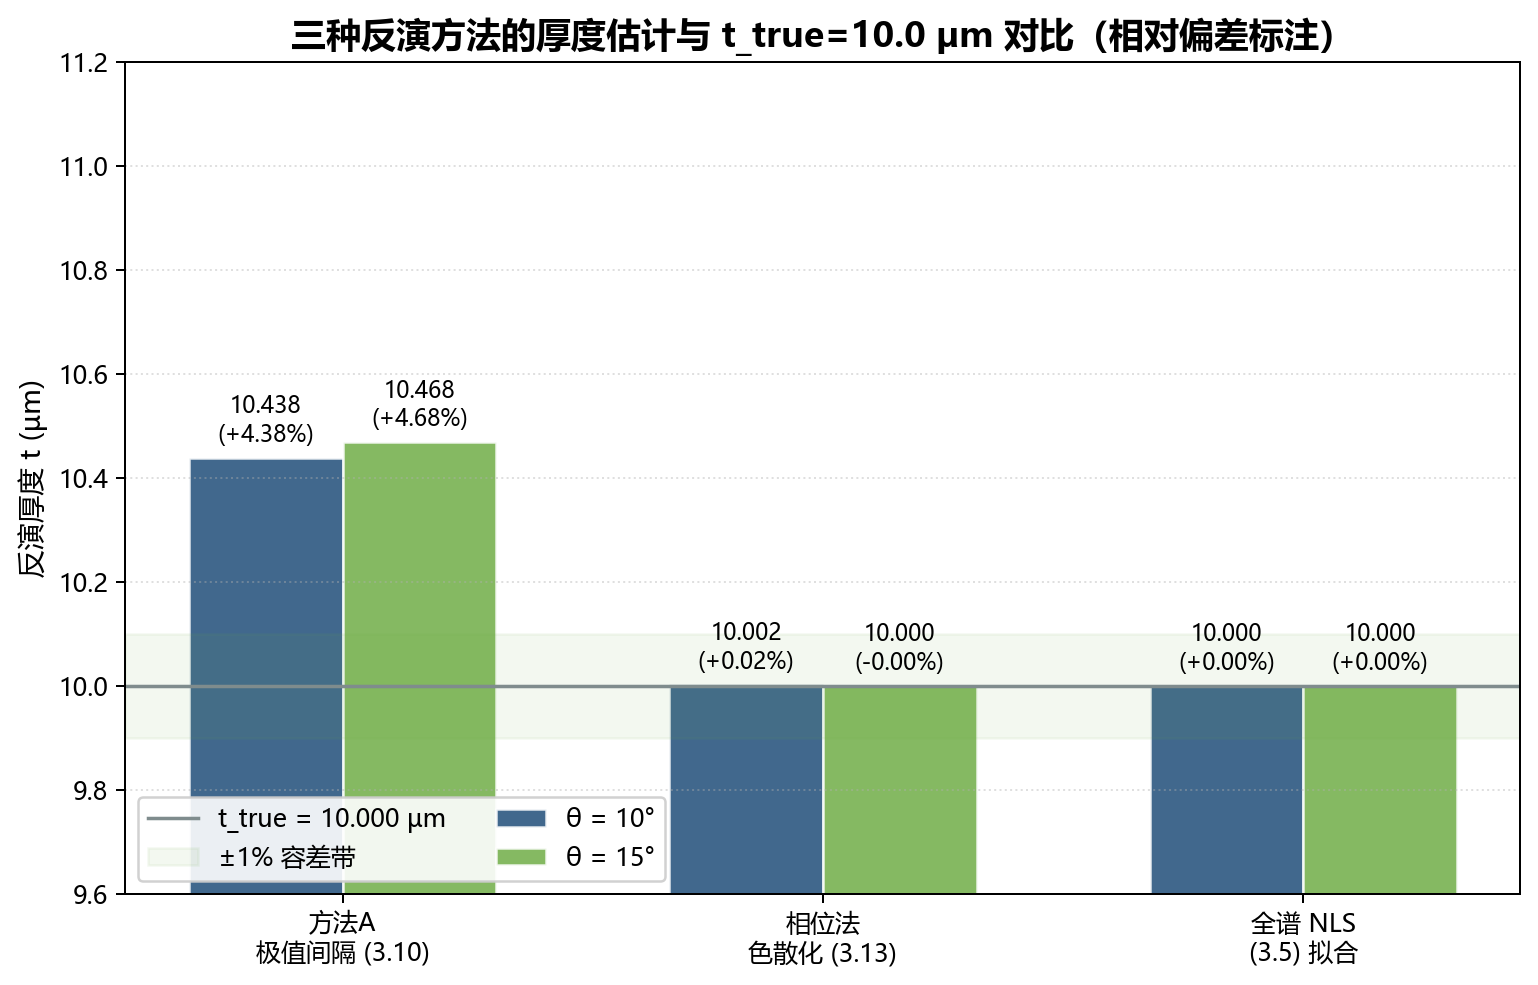
\includegraphics[keepaspectratio,alt={三种方法的合成厚度估计}]{problems/2025-cumcm-b/prob01/versions/assumption_v001/figures/prob01_fig_thickness_methods_compare_5eac465fc8.png}}

三种方法的合成厚度估计

图4
对比常数折射率间隔法、色散化相位法和全谱拟合。前者约4\%的偏差来自近似模型，后两者恢复合成真值；这里的精度不代表对实测噪声的无条件保证。

\pandocbounded{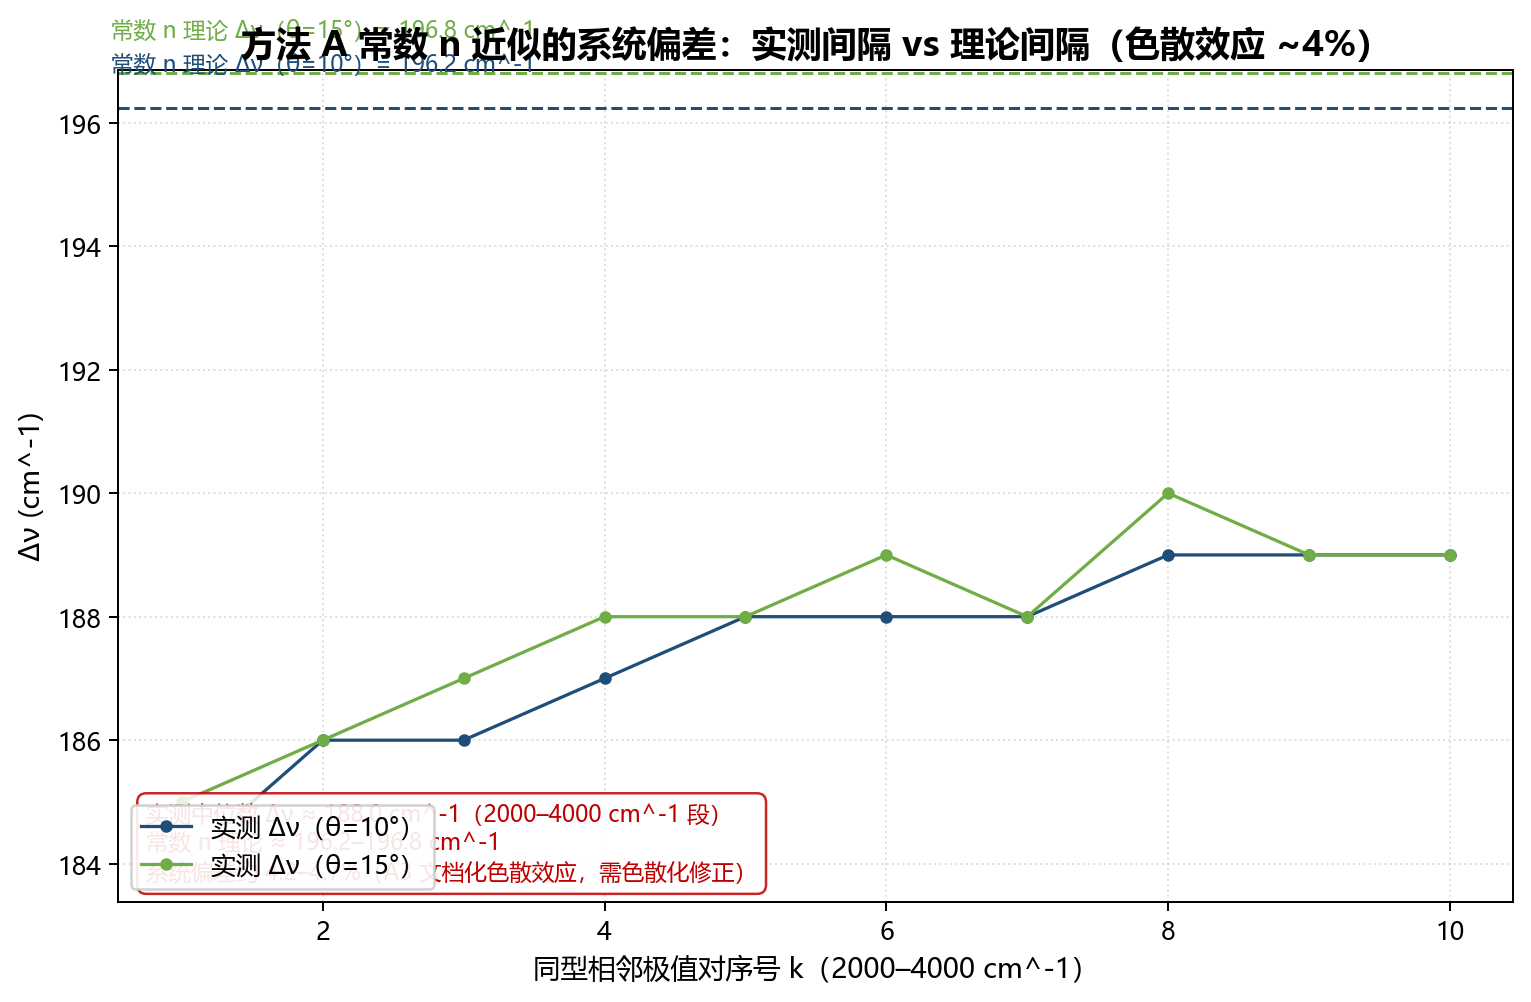
\includegraphics[keepaspectratio,alt={忽略色散时的条纹间隔偏差}]{problems/2025-cumcm-b/prob01/versions/assumption_v001/figures/prob01_fig_spacing_constant_n_bias_2245b6eda4.png}}

忽略色散时的条纹间隔偏差

图5
对比观测间隔与常数折射率近似下的理论间隔。误差具有系统性，增加相同假设下的峰数并不能消除这一偏差。

\pandocbounded{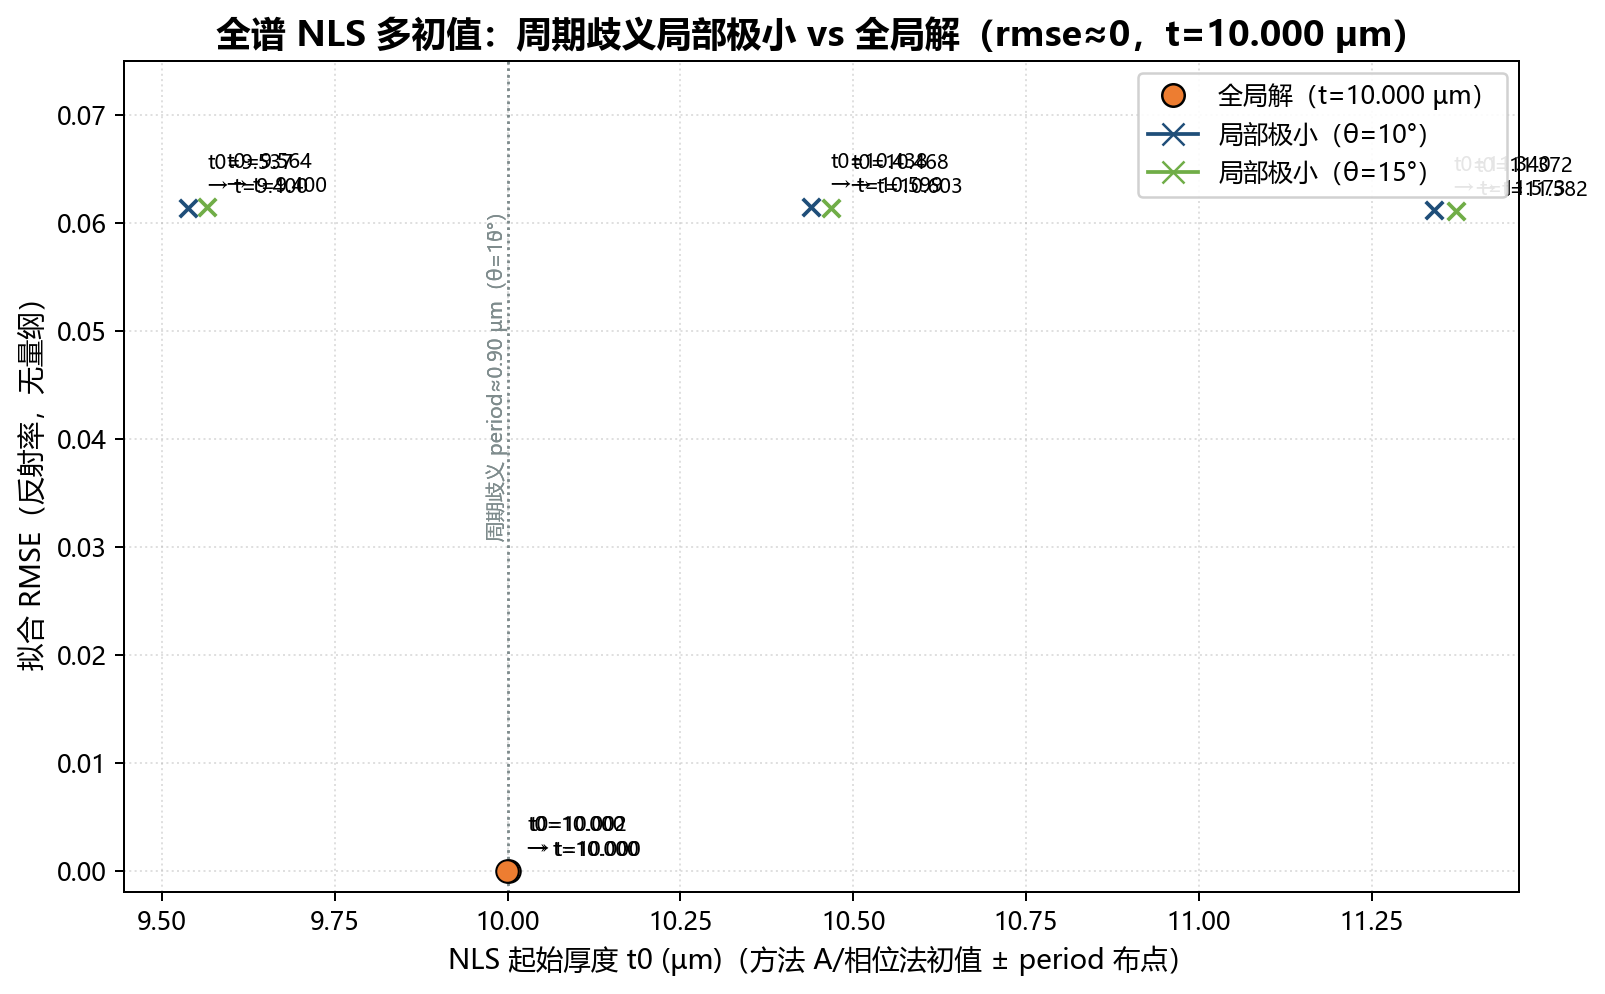
\includegraphics[keepaspectratio,alt={全谱拟合的多初值与周期歧义}]{problems/2025-cumcm-b/prob01/versions/assumption_v001/figures/prob01_fig_nls_multistart_e64919ab13.png}}

全谱拟合的多初值与周期歧义

图6
显示目标函数存在周期歧义相关的局部极小。多初值策略用于寻找较低残差的候选，不能仅凭一次局部迭代收敛就宣布找到真实厚度。

\pandocbounded{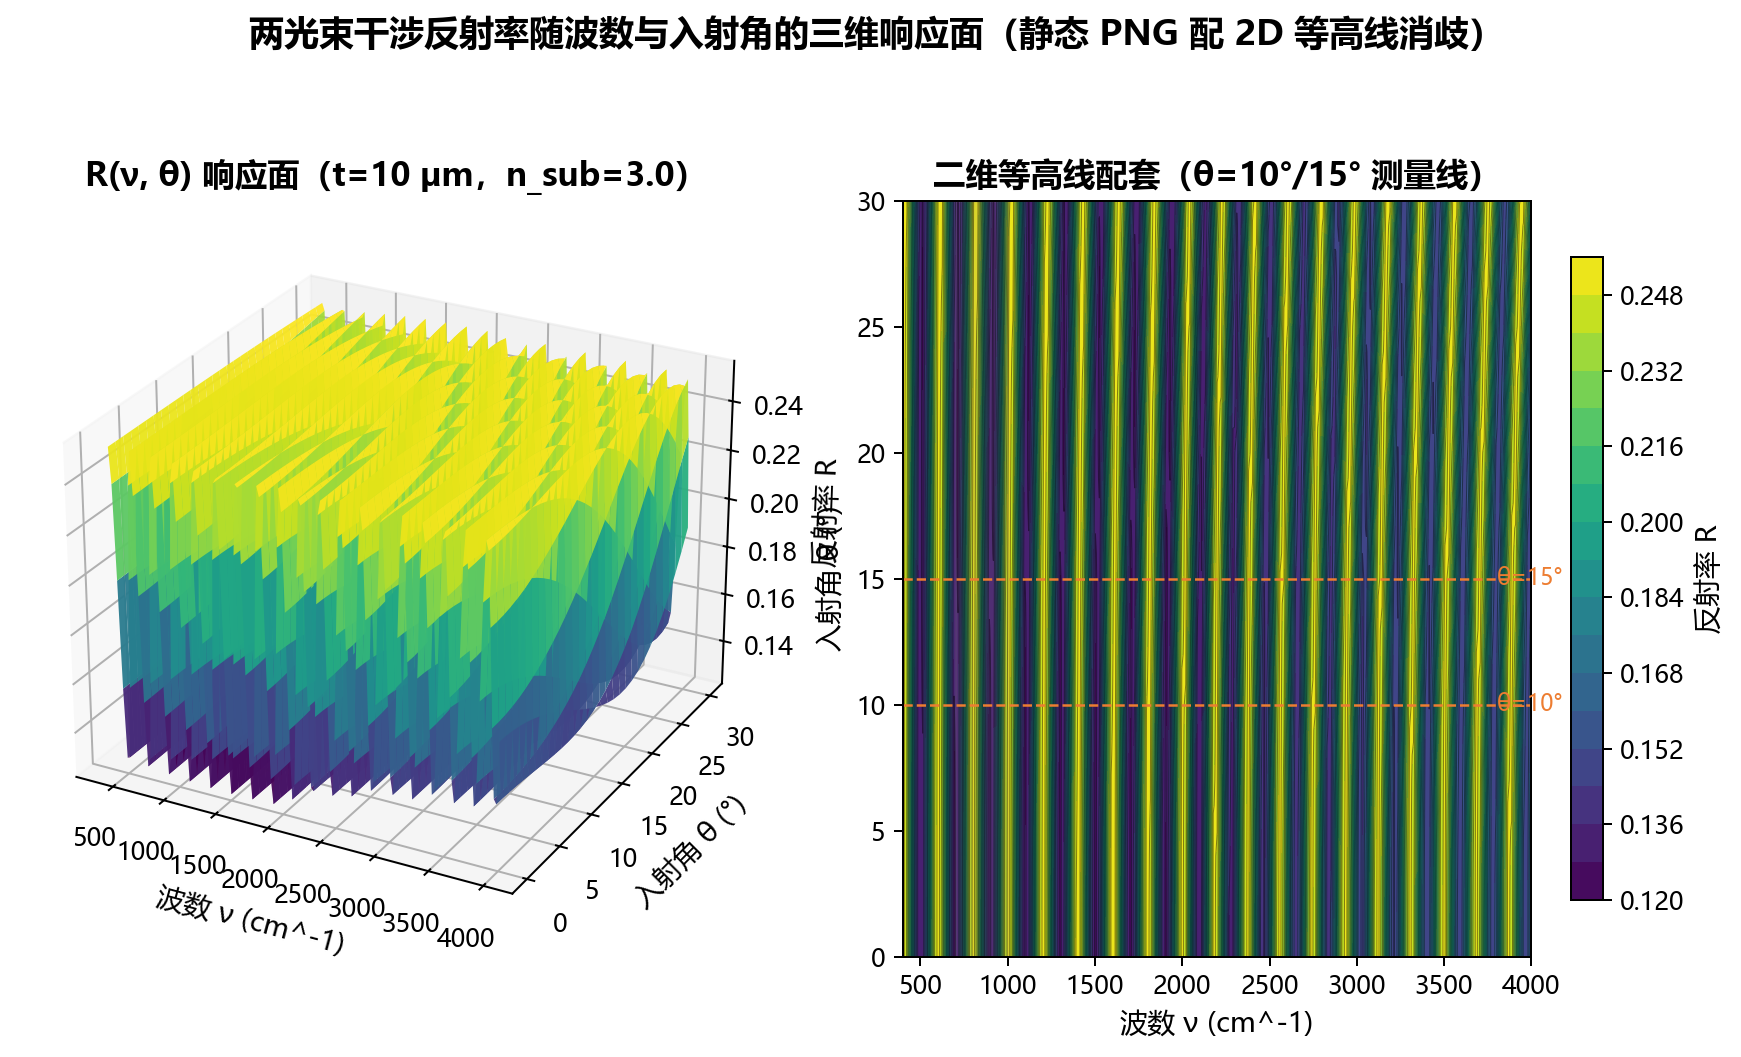
\includegraphics[keepaspectratio,alt={波数与入射角共同作用下的反射率响应}]{problems/2025-cumcm-b/prob01/versions/assumption_v001/figures/prob01_fig_response_surface_d0691c5dd8.png}}

波数与入射角共同作用下的反射率响应

图7
展示厚度固定时波数和角度对反射率的联合影响。响应面是已有模型的条件预测，不增加独立实验样本。

问题1 可靠性与结论

在既定合成场景中，衬底折射率扰动引起的最大厚度相对误差为0.008\%，角度扰动为0.22\%，替代色散模型最大偏差为0.96\%。噪声试验共600次，全部计入统计，95\%区间相对半宽最大为0.022\%。这些量评价的是指定扰动范围内的稳定性，不是材料普适误差上界。

\pandocbounded{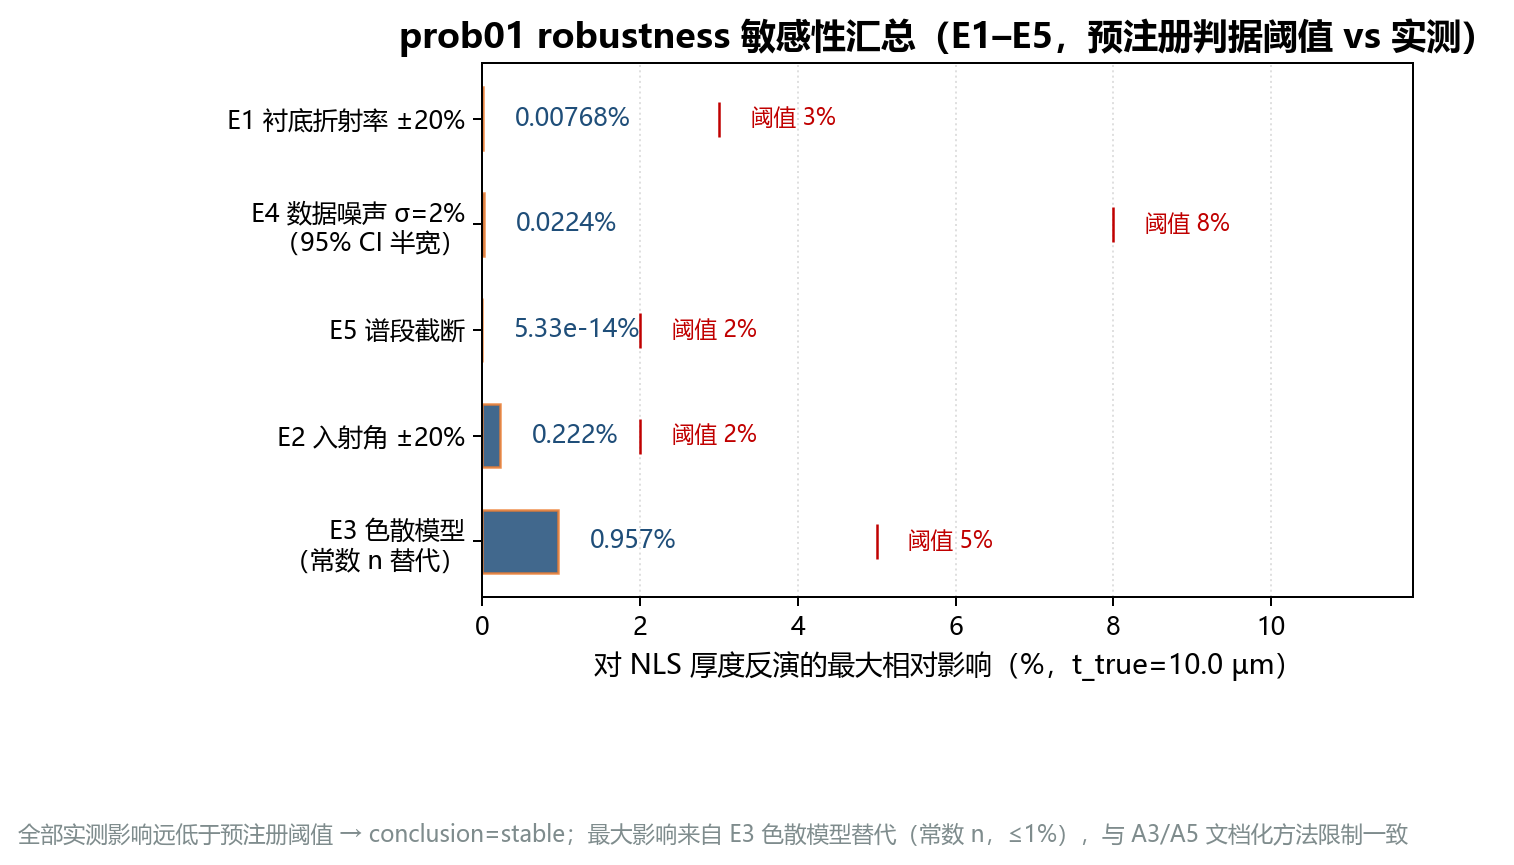
\includegraphics[keepaspectratio,alt={合成实验的参数敏感性汇总}]{problems/2025-cumcm-b/prob01/versions/assumption_v001/figures/prob01_fig_sensitivity_tornado_6983566848.png}}

合成实验的参数敏感性汇总

图8
汇总衬底折射率、角度、色散、噪声和窗口扰动结果。色散选择是需要重点控制的模型因素；各指标需与各自预设阈值比较。

\pandocbounded{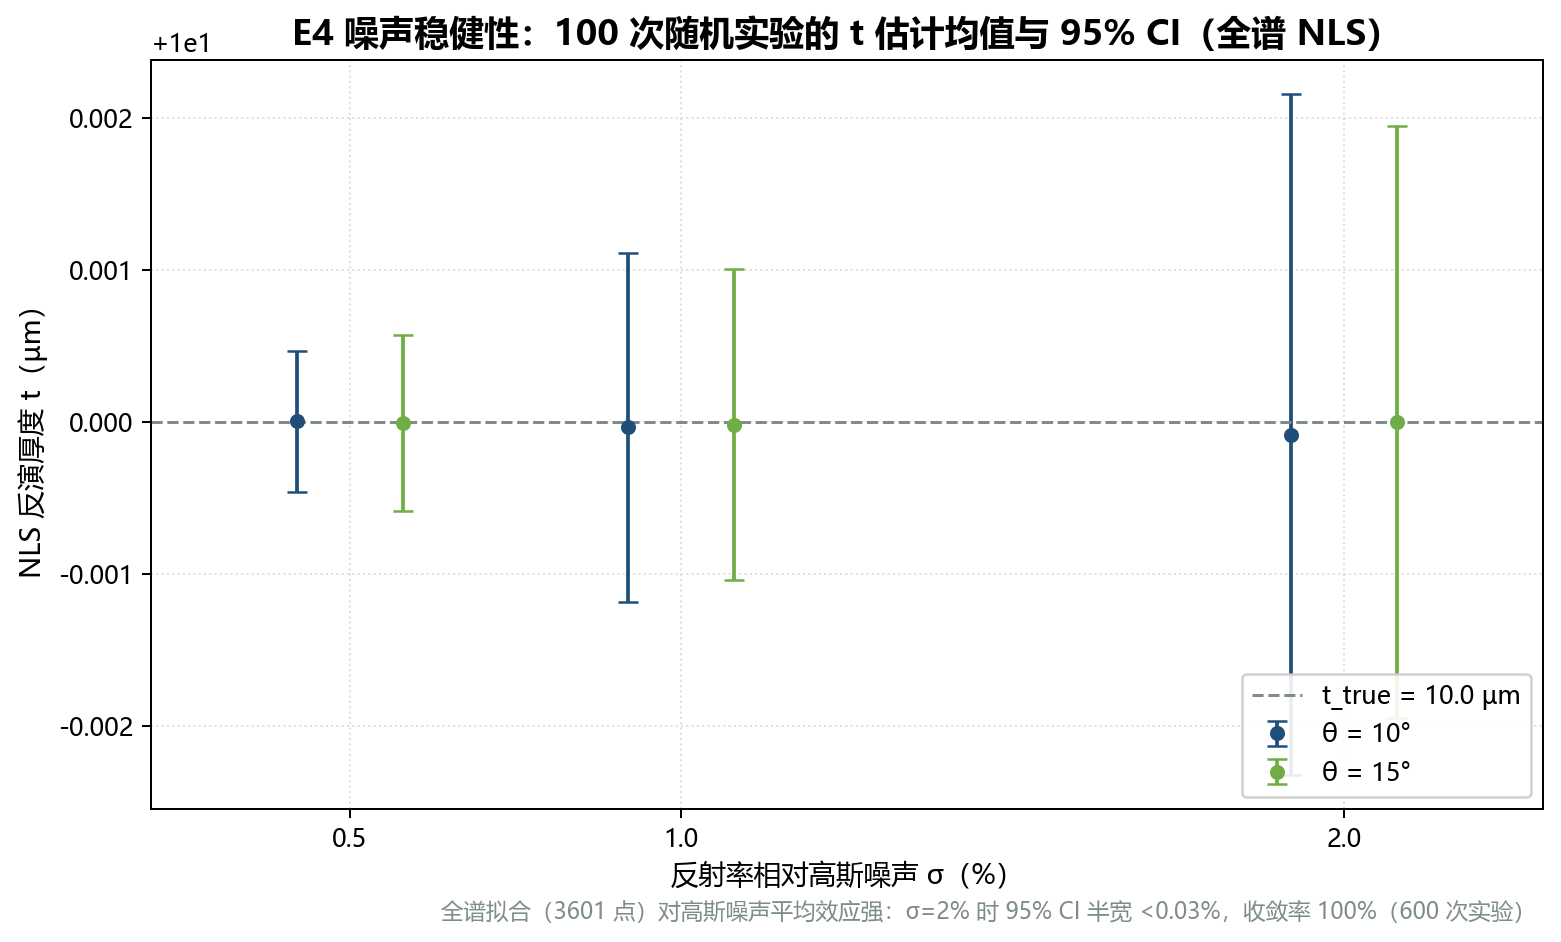
\includegraphics[keepaspectratio,alt={不同噪声水平下的合成厚度区间}]{problems/2025-cumcm-b/prob01/versions/assumption_v001/figures/prob01_fig_noise_robustness_ci_30d4fa737f.png}}

不同噪声水平下的合成厚度区间

图9
给出0.5\%、1.0\%、2.0\%噪声场景的95\%区间。全部600次重复均计入统计，最宽相对半宽为0.022\%；这仍是给定合成噪声机制下的结论。

\pandocbounded{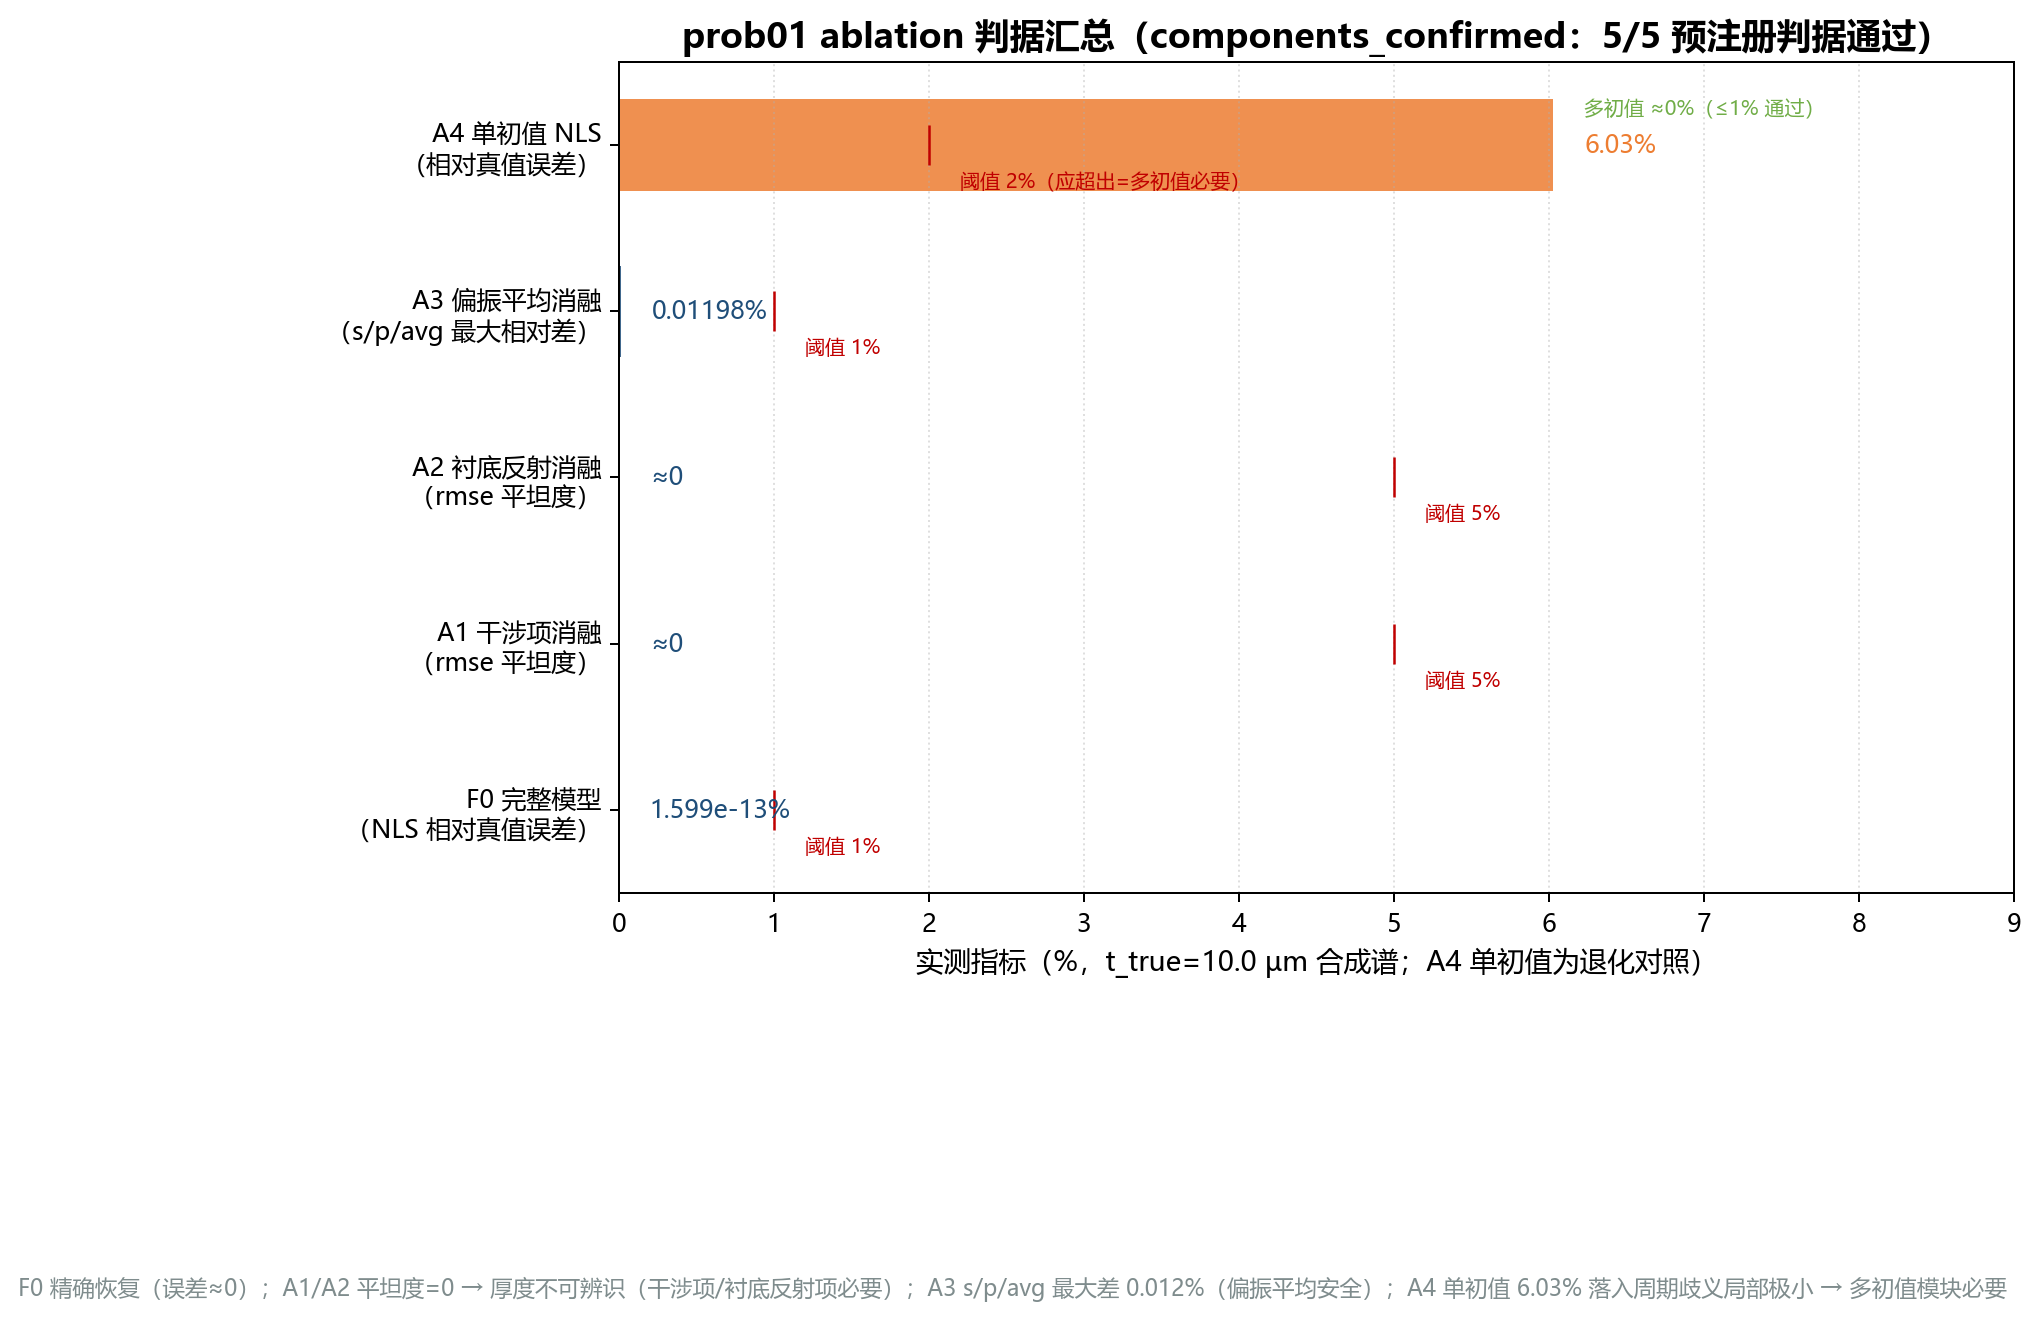
\includegraphics[keepaspectratio,alt={两光束模型的消融对照}]{problems/2025-cumcm-b/prob01/versions/assumption_v001/figures/prob01_fig_ablation_summary_ee3c34dcfa.png}}

两光束模型的消融对照

图10
汇总完整模型与移除指定组成部分后的差异。消融回答某一组成部分是否有必要，不应把所有稳定结果解释成相同的物理贡献。

\pandocbounded{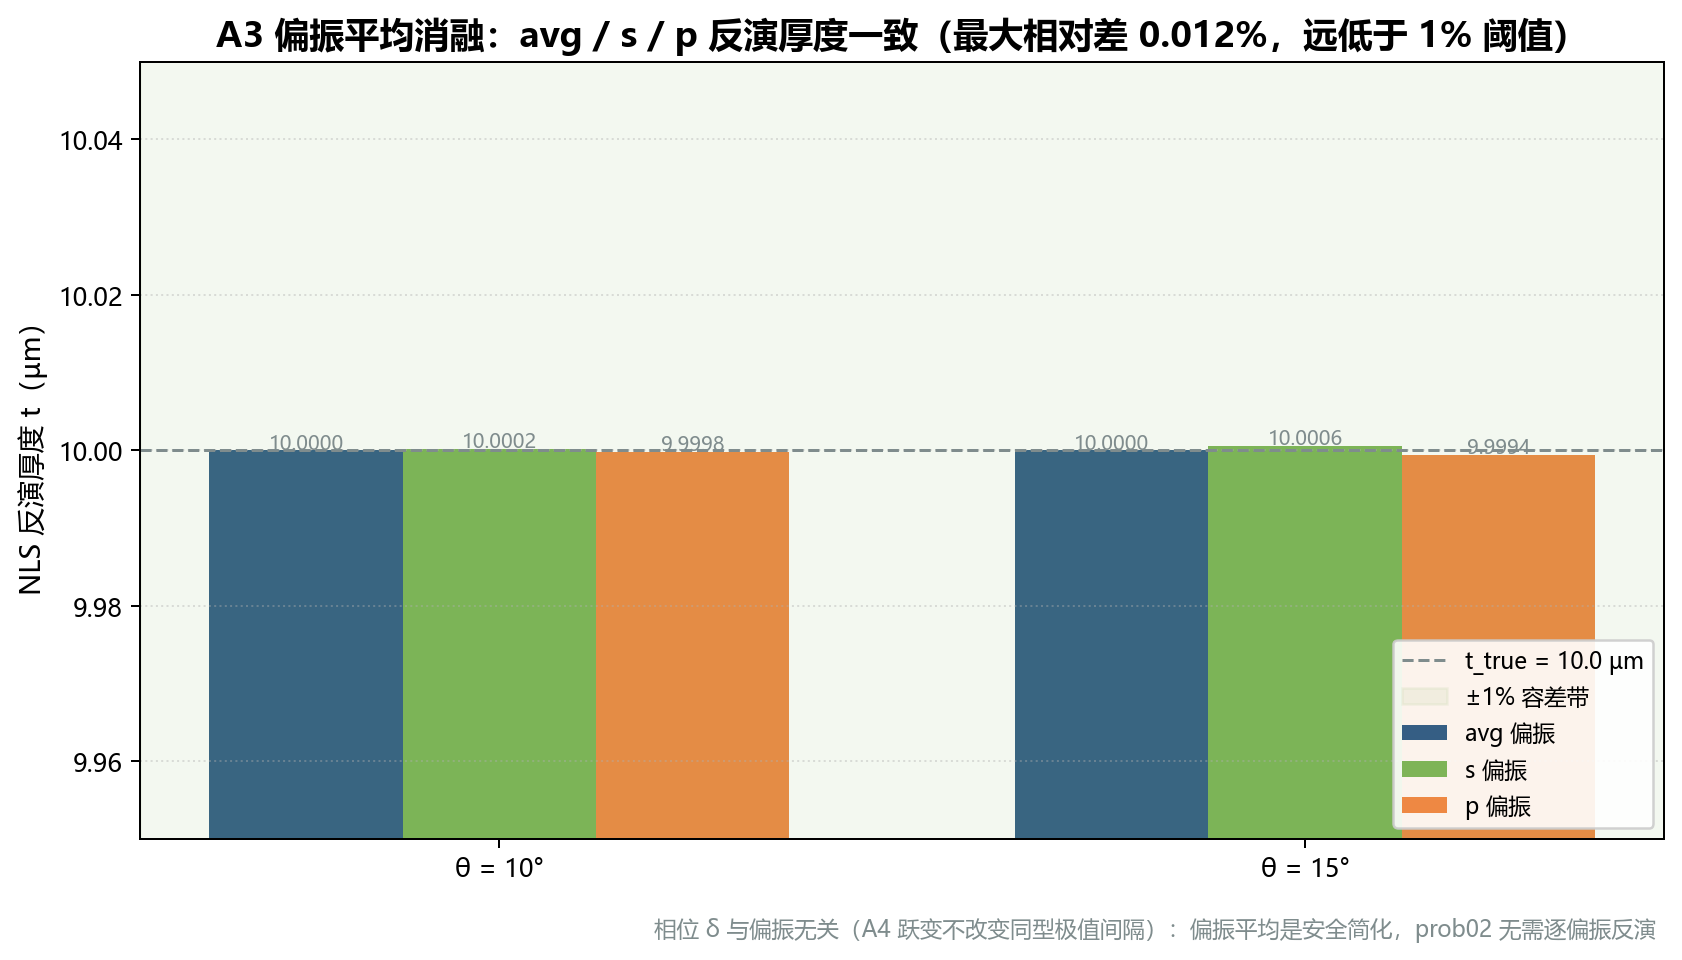
\includegraphics[keepaspectratio,alt={不同偏振处理下的合成厚度一致性}]{problems/2025-cumcm-b/prob01/versions/assumption_v001/figures/prob01_fig_ablation_polarization_da59250d1b.png}}

不同偏振处理下的合成厚度一致性

图11
对比非偏振平均与两类偏振的厚度估计。结果说明在相应正模型一致的条件下，偏振对幅度的影响不必转化为厚度偏差。

\pandocbounded{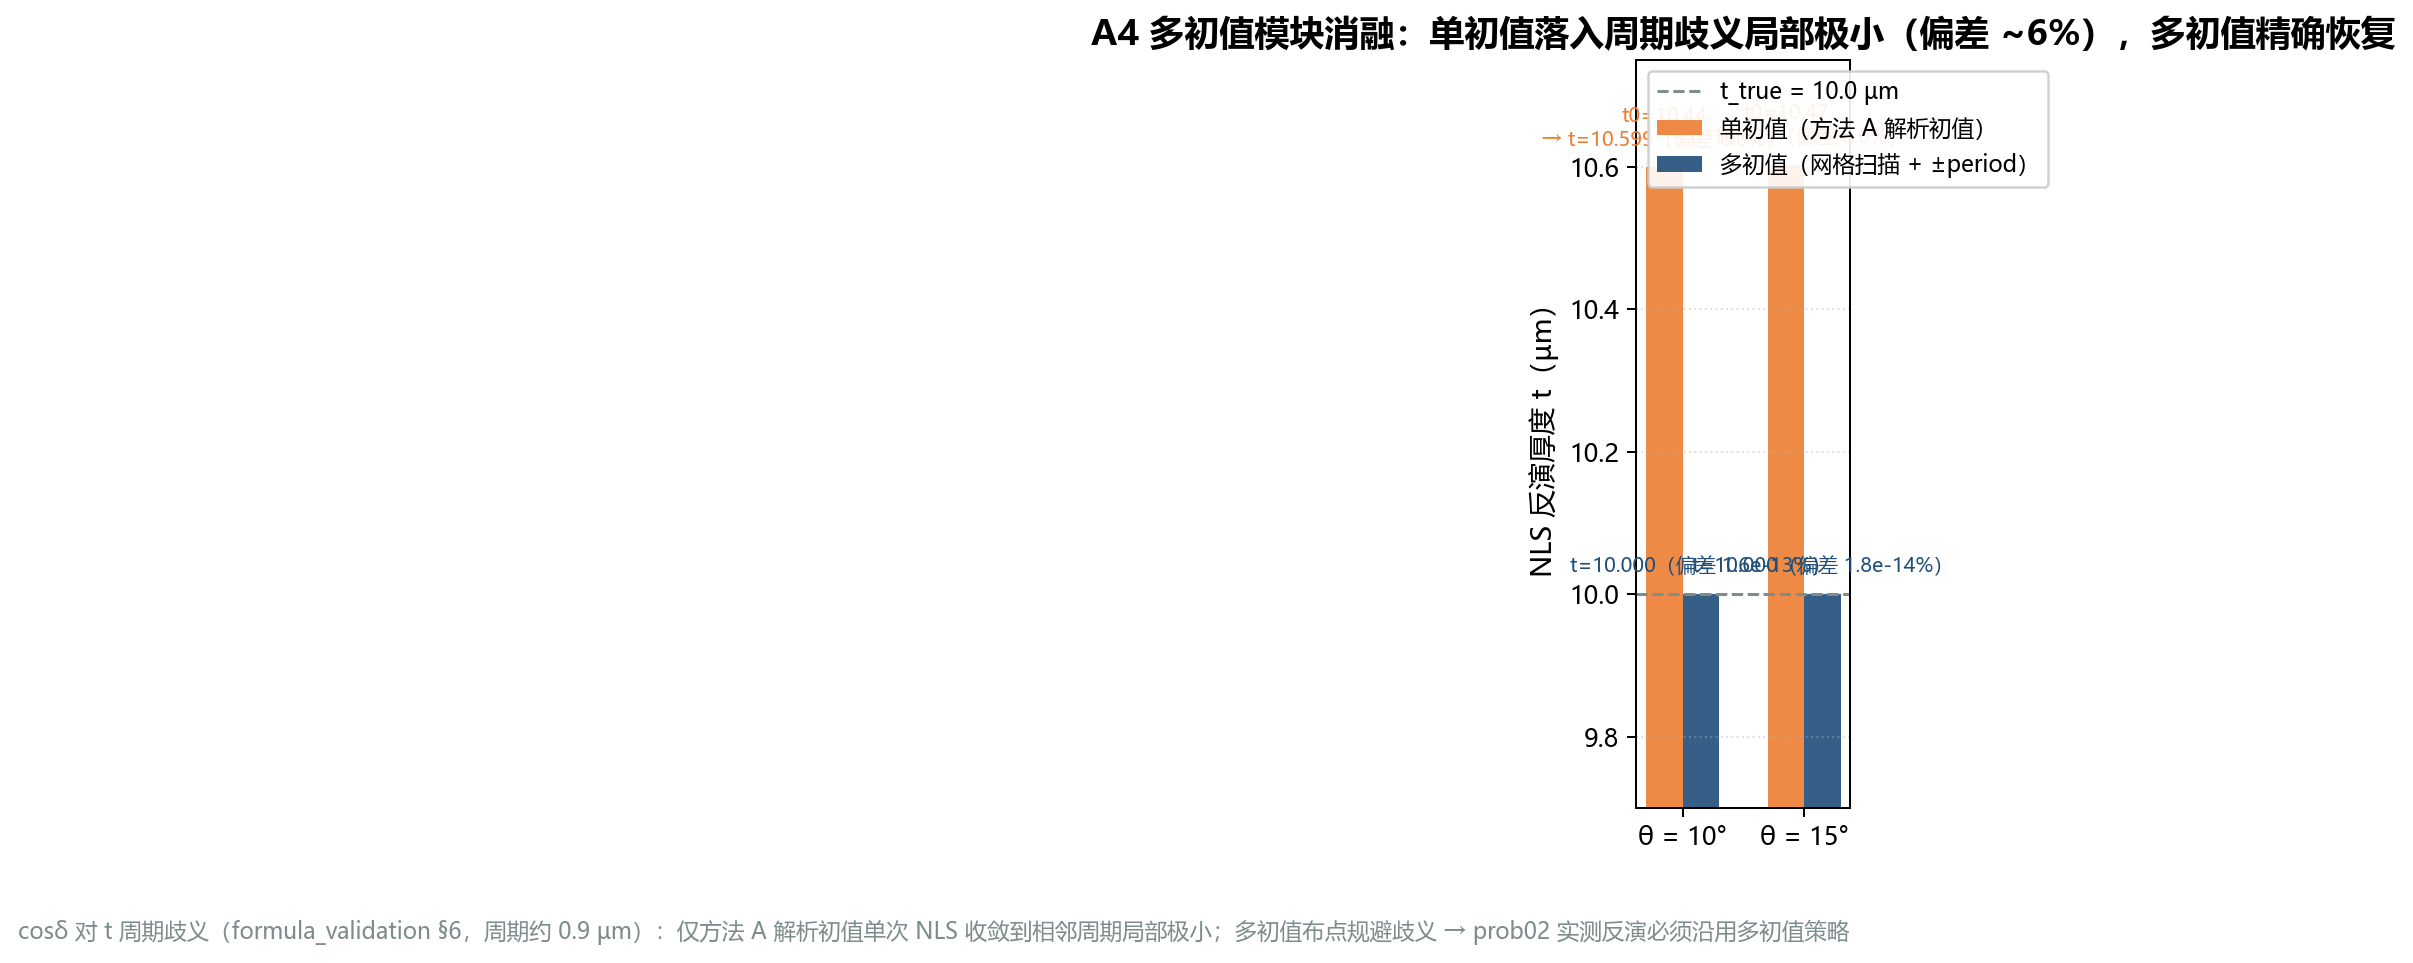
\includegraphics[keepaspectratio,alt={单初值与多初值策略对照}]{problems/2025-cumcm-b/prob01/versions/assumption_v001/figures/prob01_fig_ablation_init_strategy_7c59622d5a.png}}

单初值与多初值策略对照

图12
对比单初值落入局部极小和多初值恢复真值的结果。这为实测问题采用全区间扫描而非单次局部优化提供了算法依据。

本问支持色散修正和多候选搜索。限制是：材料色散在长波端采用常数延伸，近强吸收区须排除；衬底折射率为合成场景值；部分文献尚缺全文对照；常数折射率基线约4\%的偏差不应被隐藏。合成噪声与真实仪器误差并不等同，因此上述敏感性、置信区间和偏振对照只能作为后续实测分析的方法依据。

问题2 碳化硅实测谱的变量投影反演

问题2 问题分析

直接拟合反射率幅度会同时面对慢变背景和衬底折射率弱可辨识性；直接从所有局部极值估计周期，又可能把噪声纹波误认为干涉条纹。主方法因此将``条纹在哪里''与``条纹有多高''分离：厚度进入相位频率，基线与包络作为线性参数处理。材料吸收、掺杂与红外光学性质的相关研究用于解释适用边界，而非替代本数据的参数辨识
{[}13{]}、{[}15{]}、{[}16{]}、{[}19{]}、{[}21{]}、{[}22{]}、{[}23{]}、{[}24{]}、{[}25{]}、{[}26{]}。

问题2 模型建立与算法

对角度 \(k\) 的实测谱，写成

\[R_k^{\mathrm{obs}}(\nu_i)=B_k(\nu_i)+C_k(\nu_i)\cos\delta_k(t,\nu_i)
+S_k(\nu_i)\sin\delta_k(t,\nu_i)+\epsilon_{k,i}.\]

基线采用三阶、包络采用一阶多项式。实际实现将波数中心化并采用正交化基，以减小线性子问题的数值病态。固定厚度
\(t\) 后，设计矩阵由基线列以及乘有正弦、余弦的包络列构成，求解

\[\hat{\boldsymbol\beta}_k(t)=\arg\min_{\boldsymbol\beta_k}
\|W_k^{1/2}(\boldsymbol R_k-\Phi_k(t)\boldsymbol\beta_k)\|_2^2,\]

再对两角合并残差

\[J(t)=\sum_{k=1}^{2}\|W_k^{1/2}(\boldsymbol R_k-\Phi_k(t)\hat{\boldsymbol\beta}_k(t))\|_2^2,
\qquad \hat t=\arg\min_t J(t).\]

这使原本耦合的幅度参数在每个候选厚度处被线性消去，非线性搜索只剩一维厚度。碳化硅采用3---20
μm的既定扫描范围和0.01
μm网格，再按原程序细化候选。两角各自保留基线与包络参数，只有厚度共享；独立角度厚度通过分别最小化
\(J_k(t)\) 获得。

此处的``扫描''保证比较了指定网格与范围内的候选，并不等于对所有材料参数及无限厚度区间证明全局可辨识。与既有色散修正及全谱拟合研究相对照
{[}17{]}、{[}20{]}、{[}27{]}，本文更强调分离相位和背景后对真实数据的可解释性。

问题2 厚度结果与对照

碳化硅实测厚度估计

\begin{longtable}[]{@{}lll@{}}
\toprule\noalign{}
估计对象 & 厚度/μm & 解释 \\
\midrule\noalign{}
\endhead
\bottomrule\noalign{}
\endlastfoot
两角共享 & 7.2158 & 本文报告的共同厚度 \\
10°独立估计 & 7.2214 & 用于角度一致性对照 \\
15°独立估计 & 7.2095 & 用于角度一致性对照 \\
\end{longtable}

角度相对差为0.165\%。轮廓似然95\%区间的相对半宽约0.0911\%，它是在当前噪声、色散和模型设定下的条件区间；没有执行残差重采样，故不称为自助法区间，也不覆盖全部系统误差。

\pandocbounded{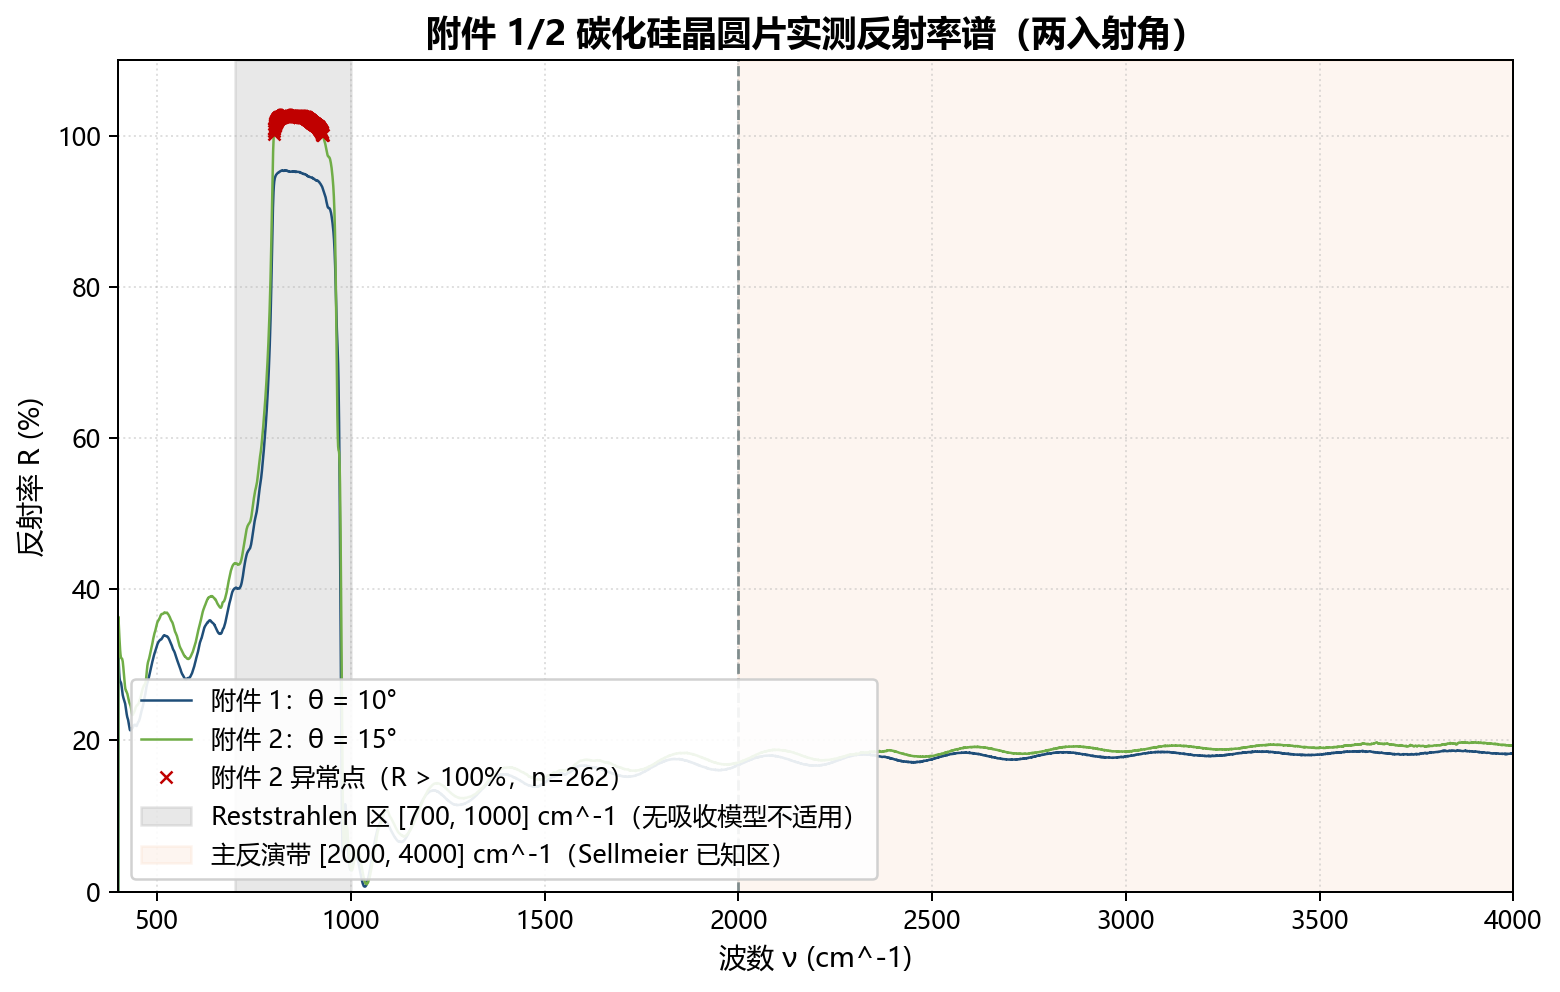
\includegraphics[keepaspectratio,alt={碳化硅两入射角实测反射率谱}]{problems/2025-cumcm-b/prob02/versions/assumption_v001/figures/prob02_fig_reflectance_spectrum_6b2265d217.png}}

碳化硅两入射角实测反射率谱

图13
给出附件1、2的测量谱线。数据同时含慢变背景与干涉纹波，异常反射率点及强吸收谱段需在反演前按既定规则处理。

\pandocbounded{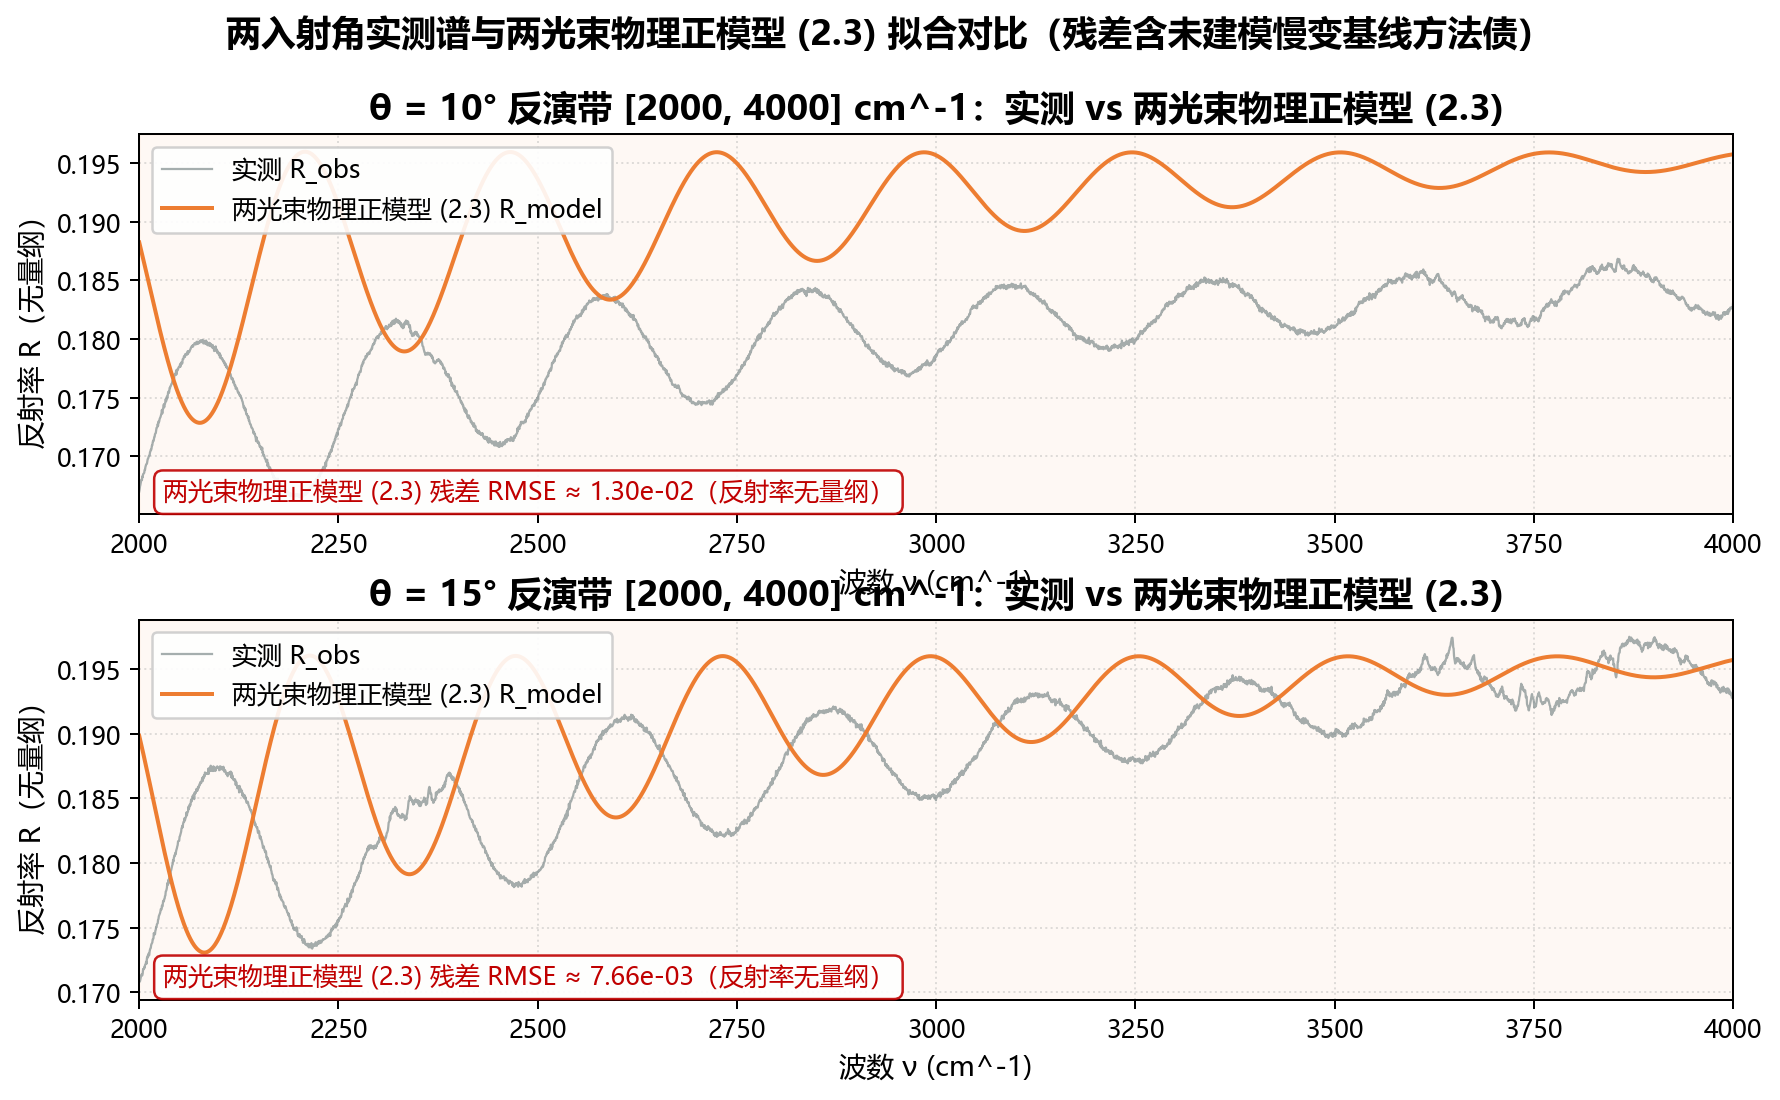
\includegraphics[keepaspectratio,alt={碳化硅实测谱与物理两光束诊断拟合}]{problems/2025-cumcm-b/prob02/versions/assumption_v001/figures/prob02_fig_model_fit_0ca711689b.png}}

碳化硅实测谱与物理两光束诊断拟合

图14
对比实测谱与刚性Fresnel基线下的物理正模型。此图用于诊断，不能把它的残差当成变量投影主方法的残差；两种基线定义不同。

\pandocbounded{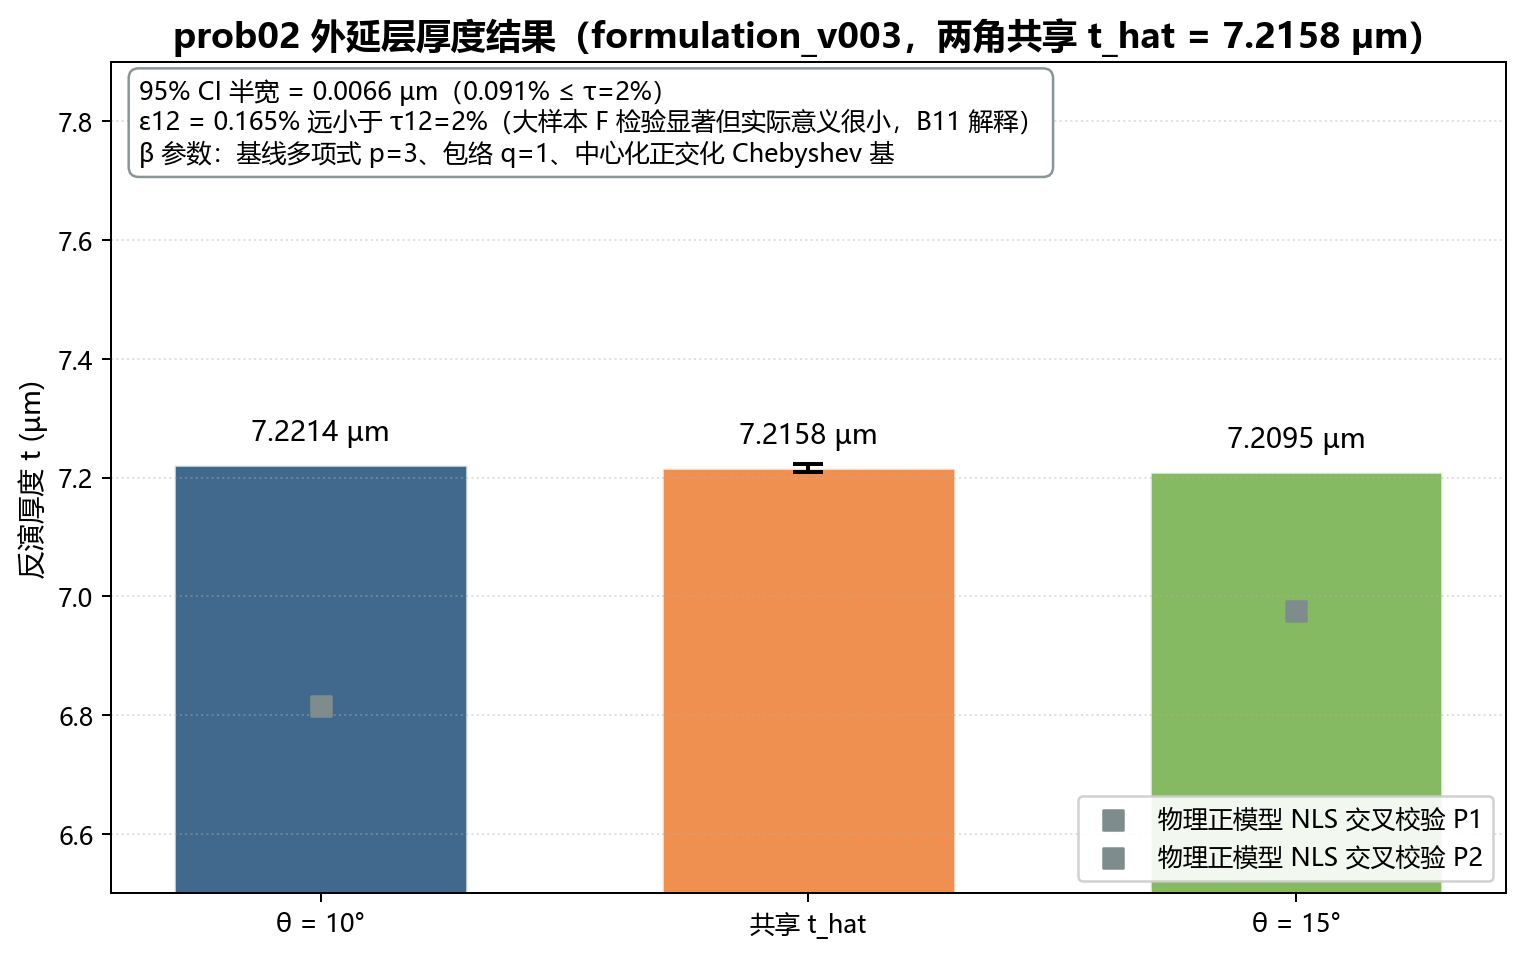
\includegraphics[keepaspectratio,alt={碳化硅共享厚度与分角度厚度估计}]{problems/2025-cumcm-b/prob02/versions/assumption_v001/figures/prob02_fig_thickness_estimate_efa7359eb9.png}}

碳化硅共享厚度与分角度厚度估计

图15 展示两角共享7.2158 μm以及分角度7.2214、7.2095
μm的结果。0.165\%的相对差小于工程阈值，但统计F检验仍提示角度间存在可检测差异。

\pandocbounded{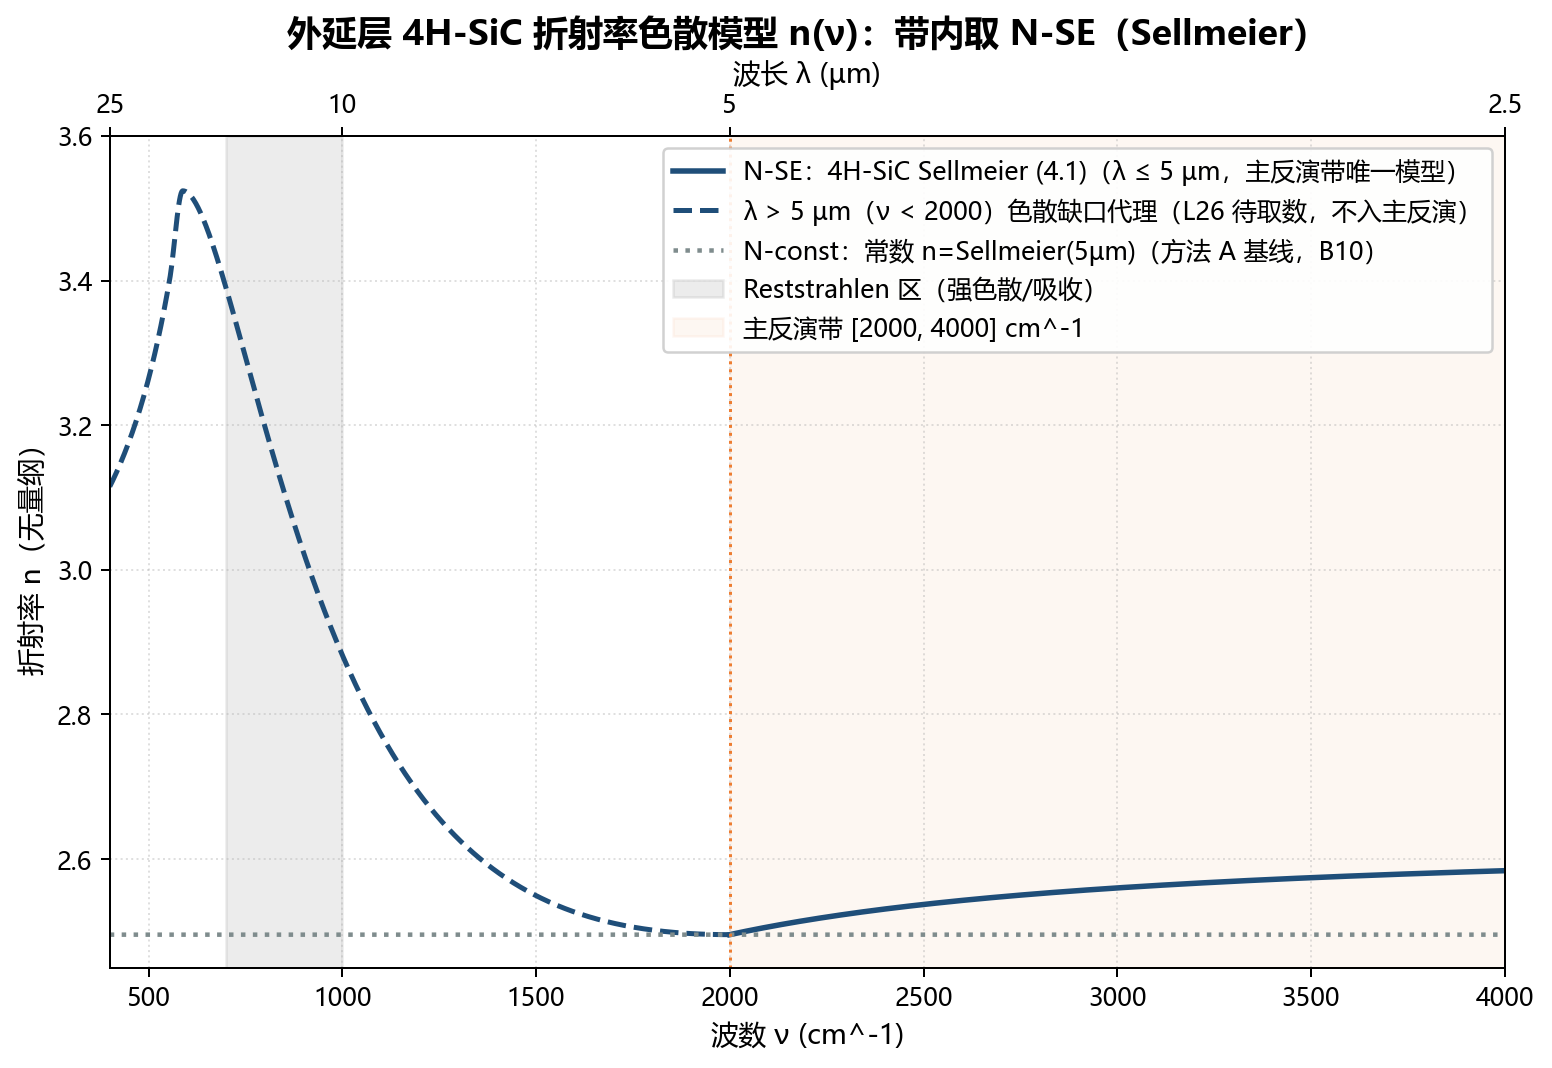
\includegraphics[keepaspectratio,alt={碳化硅主反演带内的色散模型}]{problems/2025-cumcm-b/prob02/versions/assumption_v001/figures/prob02_fig_dispersion_curve_af50244106.png}}

碳化硅主反演带内的色散模型

图16 给出主反演使用的折射率变化。波数低于2000
cm⁻¹时的材料色散信息缺口不能靠延长同一公式来消除。

\pandocbounded{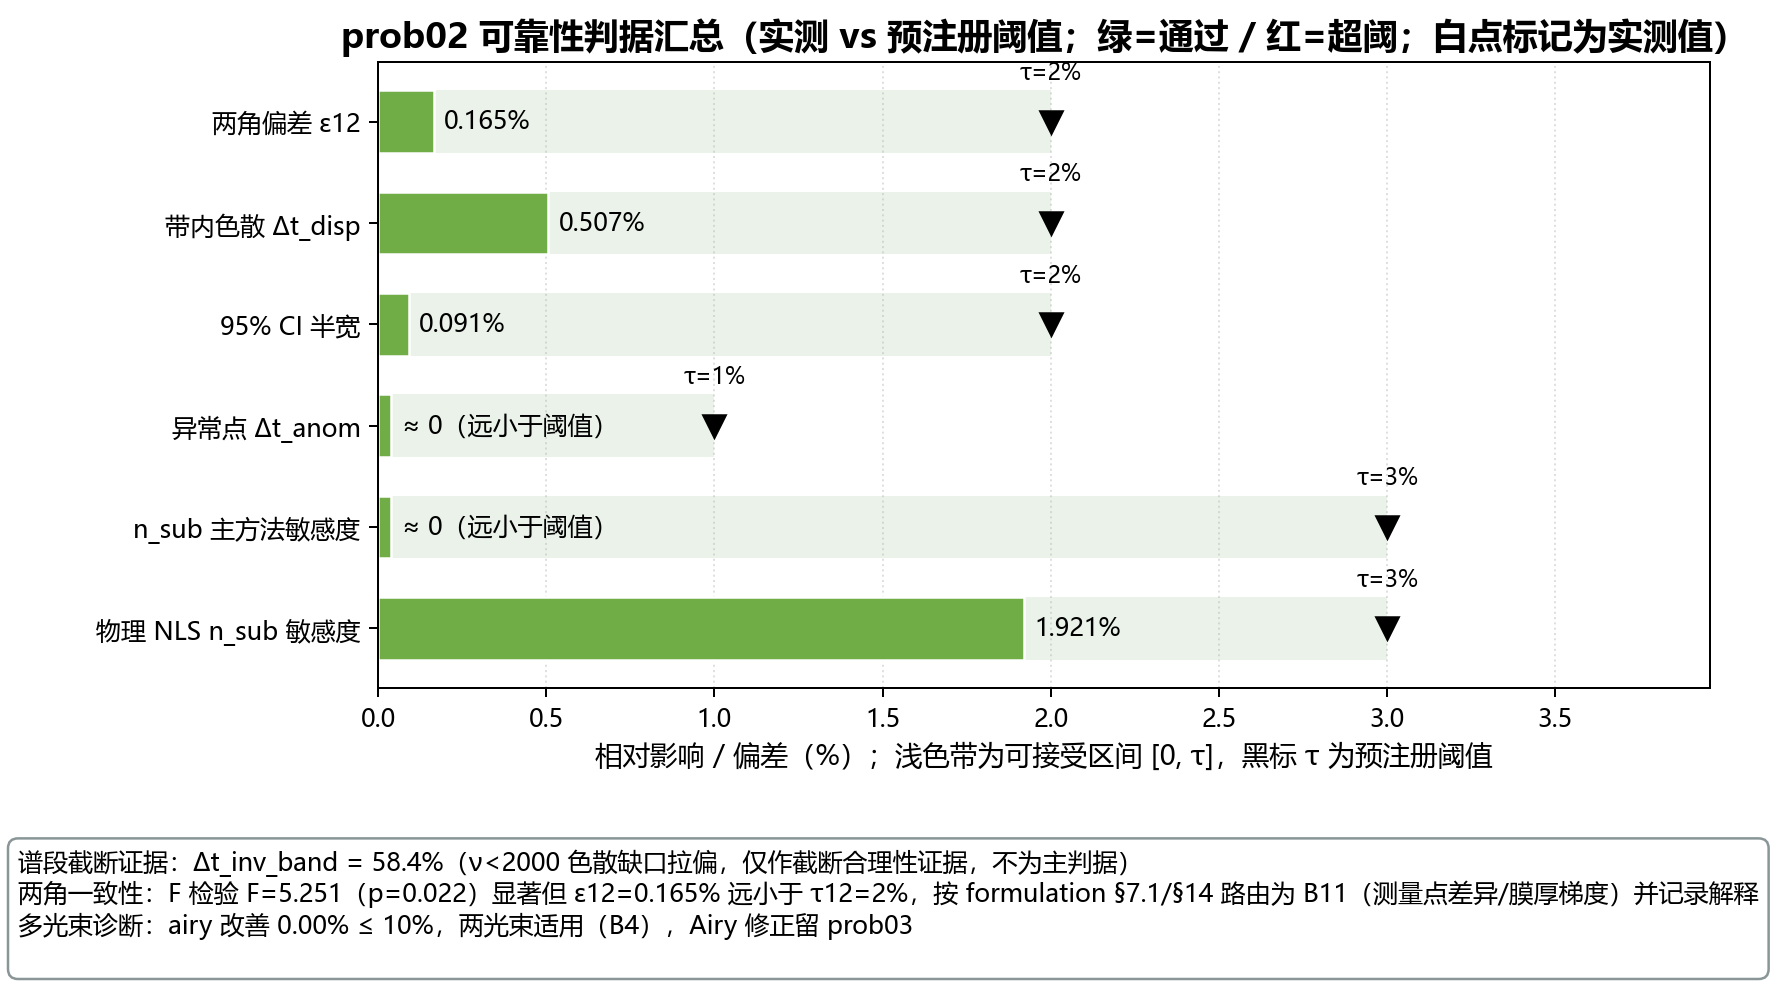
\includegraphics[keepaspectratio,alt={碳化硅可靠性指标与预设阈值}]{problems/2025-cumcm-b/prob02/versions/assumption_v001/figures/prob02_fig_reliability_summary_78cd97014b.png}}

碳化硅可靠性指标与预设阈值

图17
汇总不同误差来源的检验。两角F检验的拒绝结果应与0.165\%的实际偏差同时解释，不能合并为``所有统计检验均通过''。

\pandocbounded{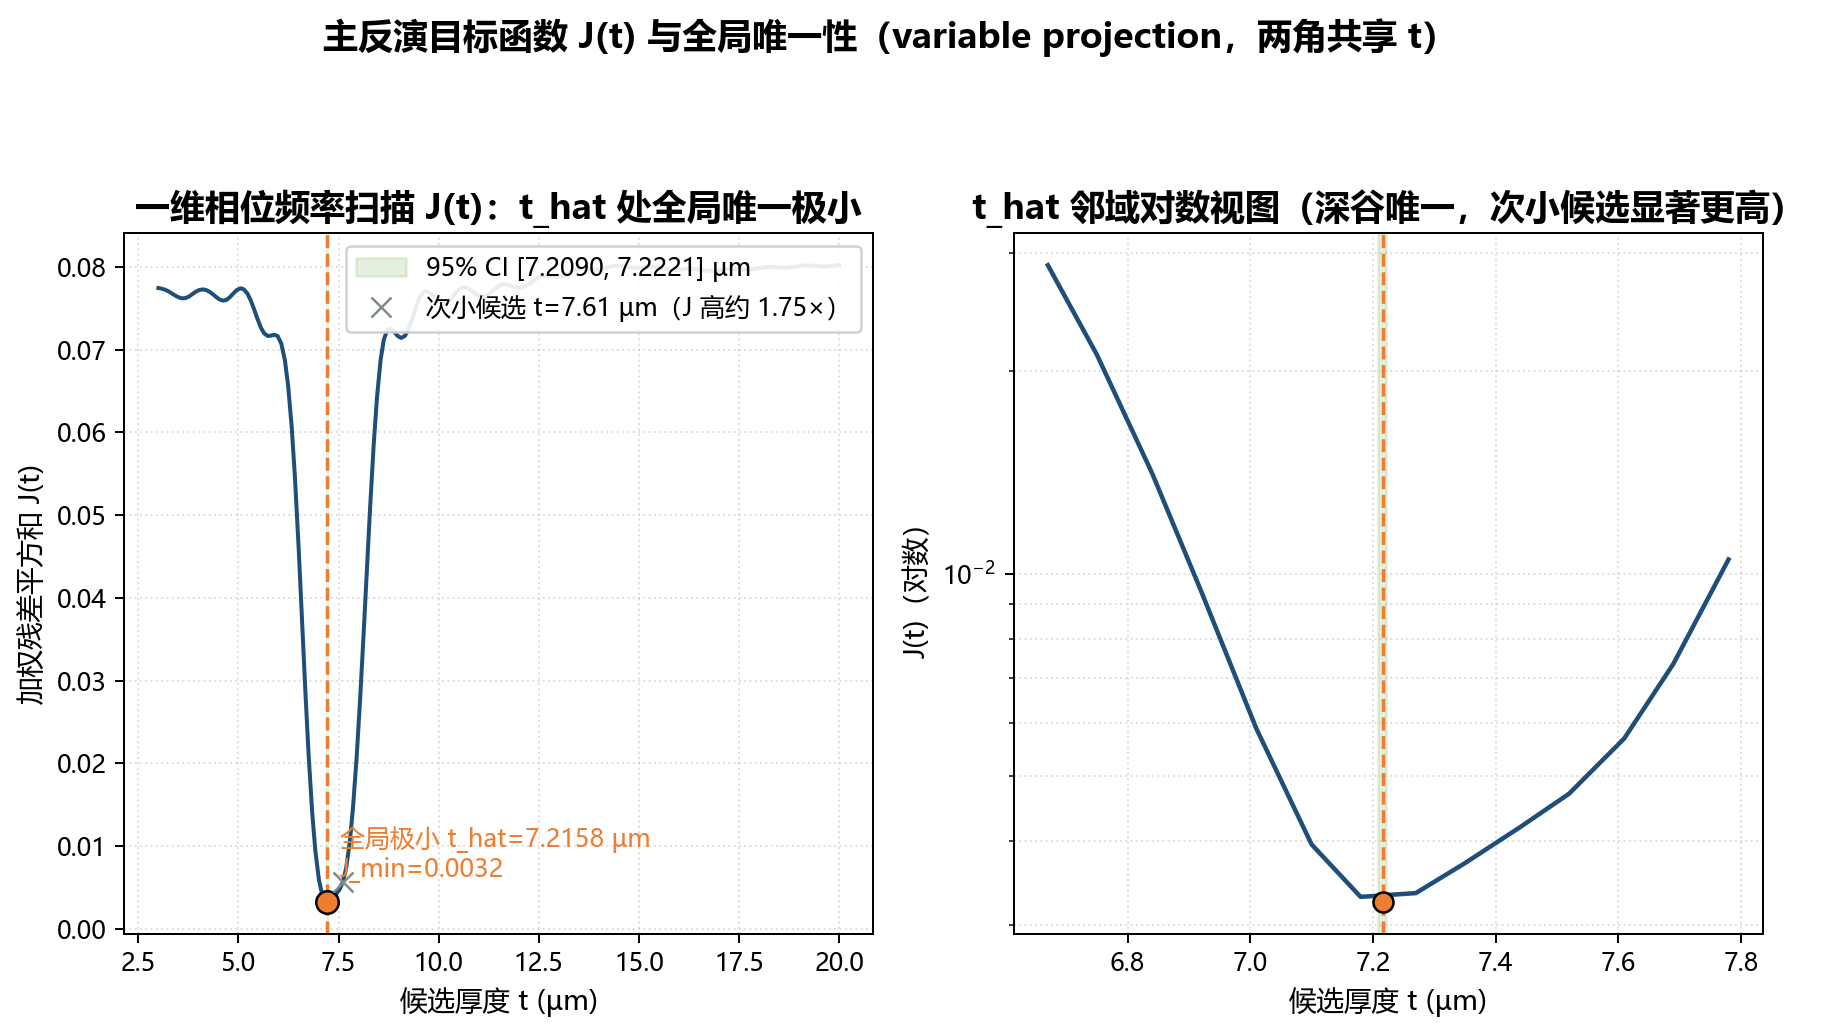
\includegraphics[keepaspectratio,alt={碳化硅一维厚度目标函数}]{problems/2025-cumcm-b/prob02/versions/assumption_v001/figures/prob02_fig_variable_projection_jcurve_7a9a903650.png}}

碳化硅一维厚度目标函数

图18
显示厚度扫描对应的目标函数及候选极小值。全区间比较补充了局部优化无法提供的周期歧义检查。

\pandocbounded{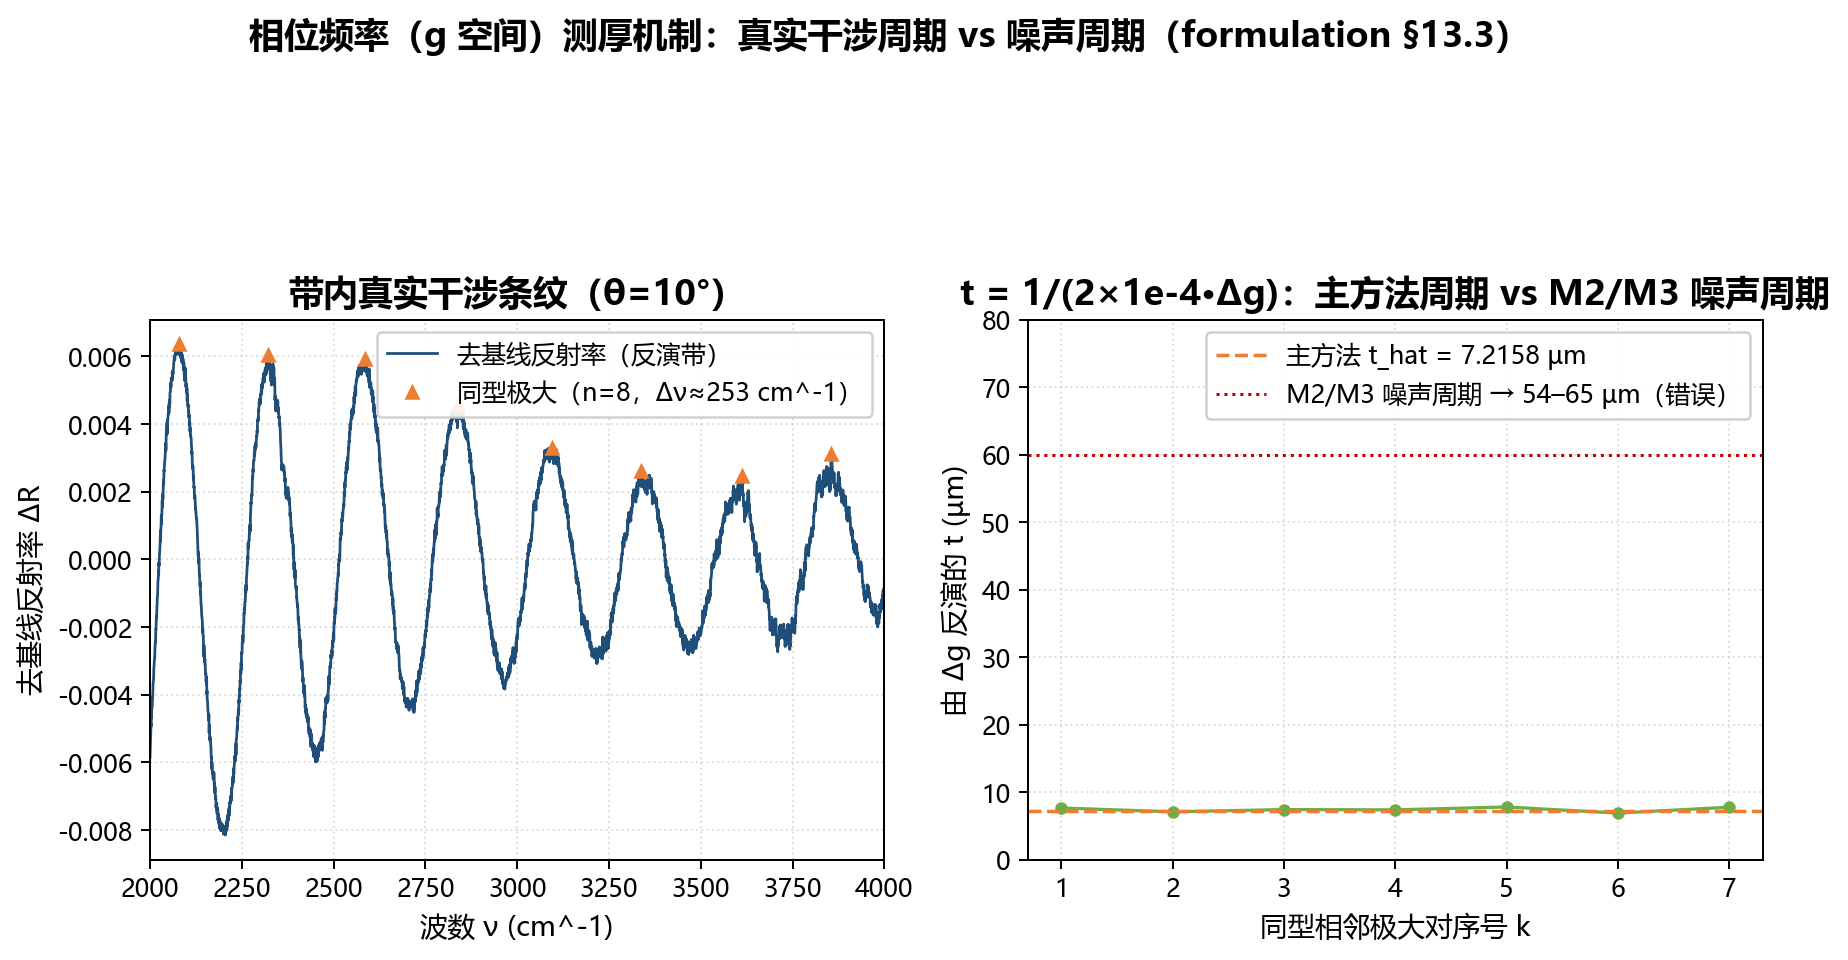
\includegraphics[keepaspectratio,alt={碳化硅相位坐标与噪声极值辨别}]{problems/2025-cumcm-b/prob02/versions/assumption_v001/figures/prob02_fig_g_space_phase_gap_f500d9c0db.png}}

碳化硅相位坐标与噪声极值辨别

图19
对比真实干涉周期和噪声纹波的极值计数。直接使用细密噪声极值会产生约54---65
μm的错误厚度量级，因此不作为主结果。

\pandocbounded{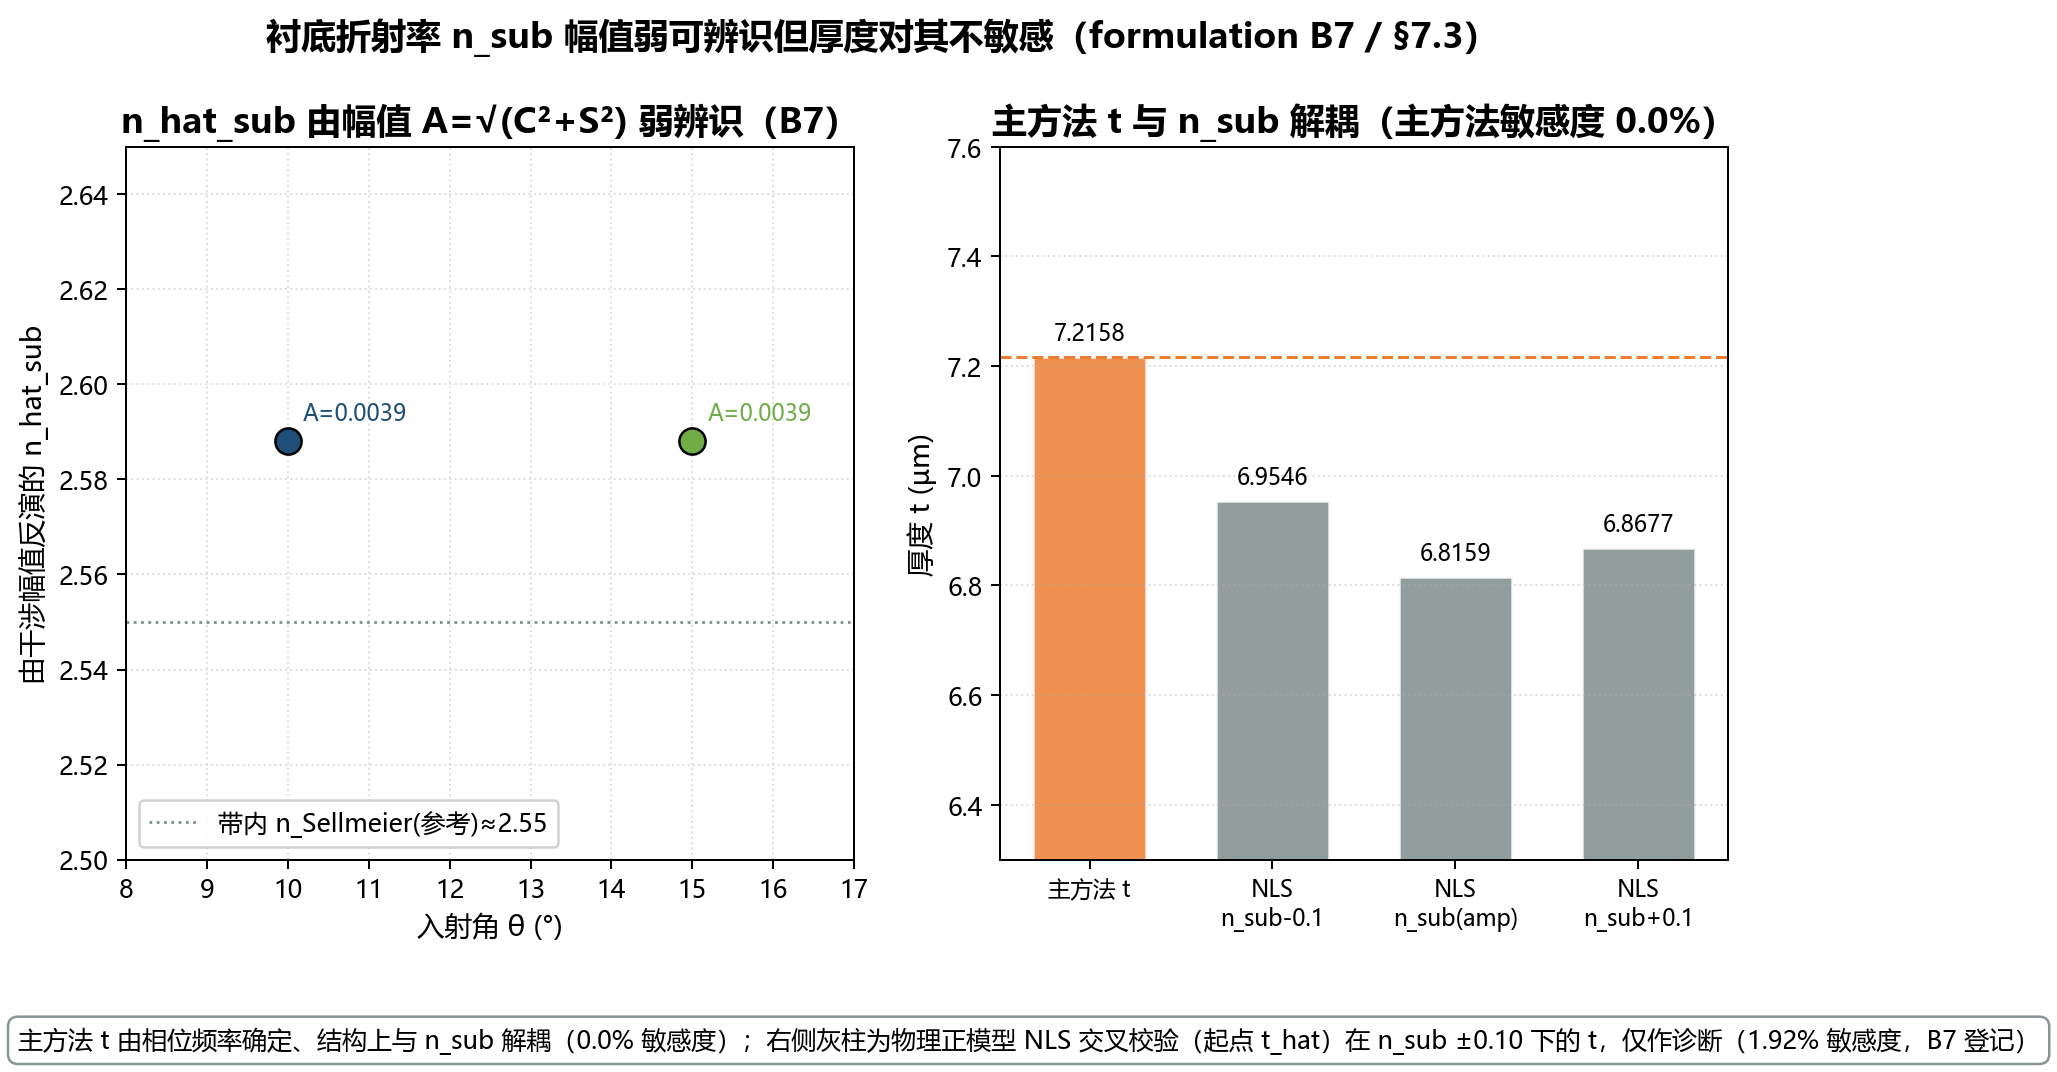
\includegraphics[keepaspectratio,alt={厚度与衬底折射率的结构解耦}]{problems/2025-cumcm-b/prob02/versions/assumption_v001/figures/prob02_fig_nsub_decoupling_39b4128d09.png}}

厚度与衬底折射率的结构解耦

图20
展示相位频率决定厚度、幅度承担衬底折射率信息的分工。结构解耦降低了幅度弱可辨识对厚度的传递，但不意味着衬底折射率已精确测定。

\pandocbounded{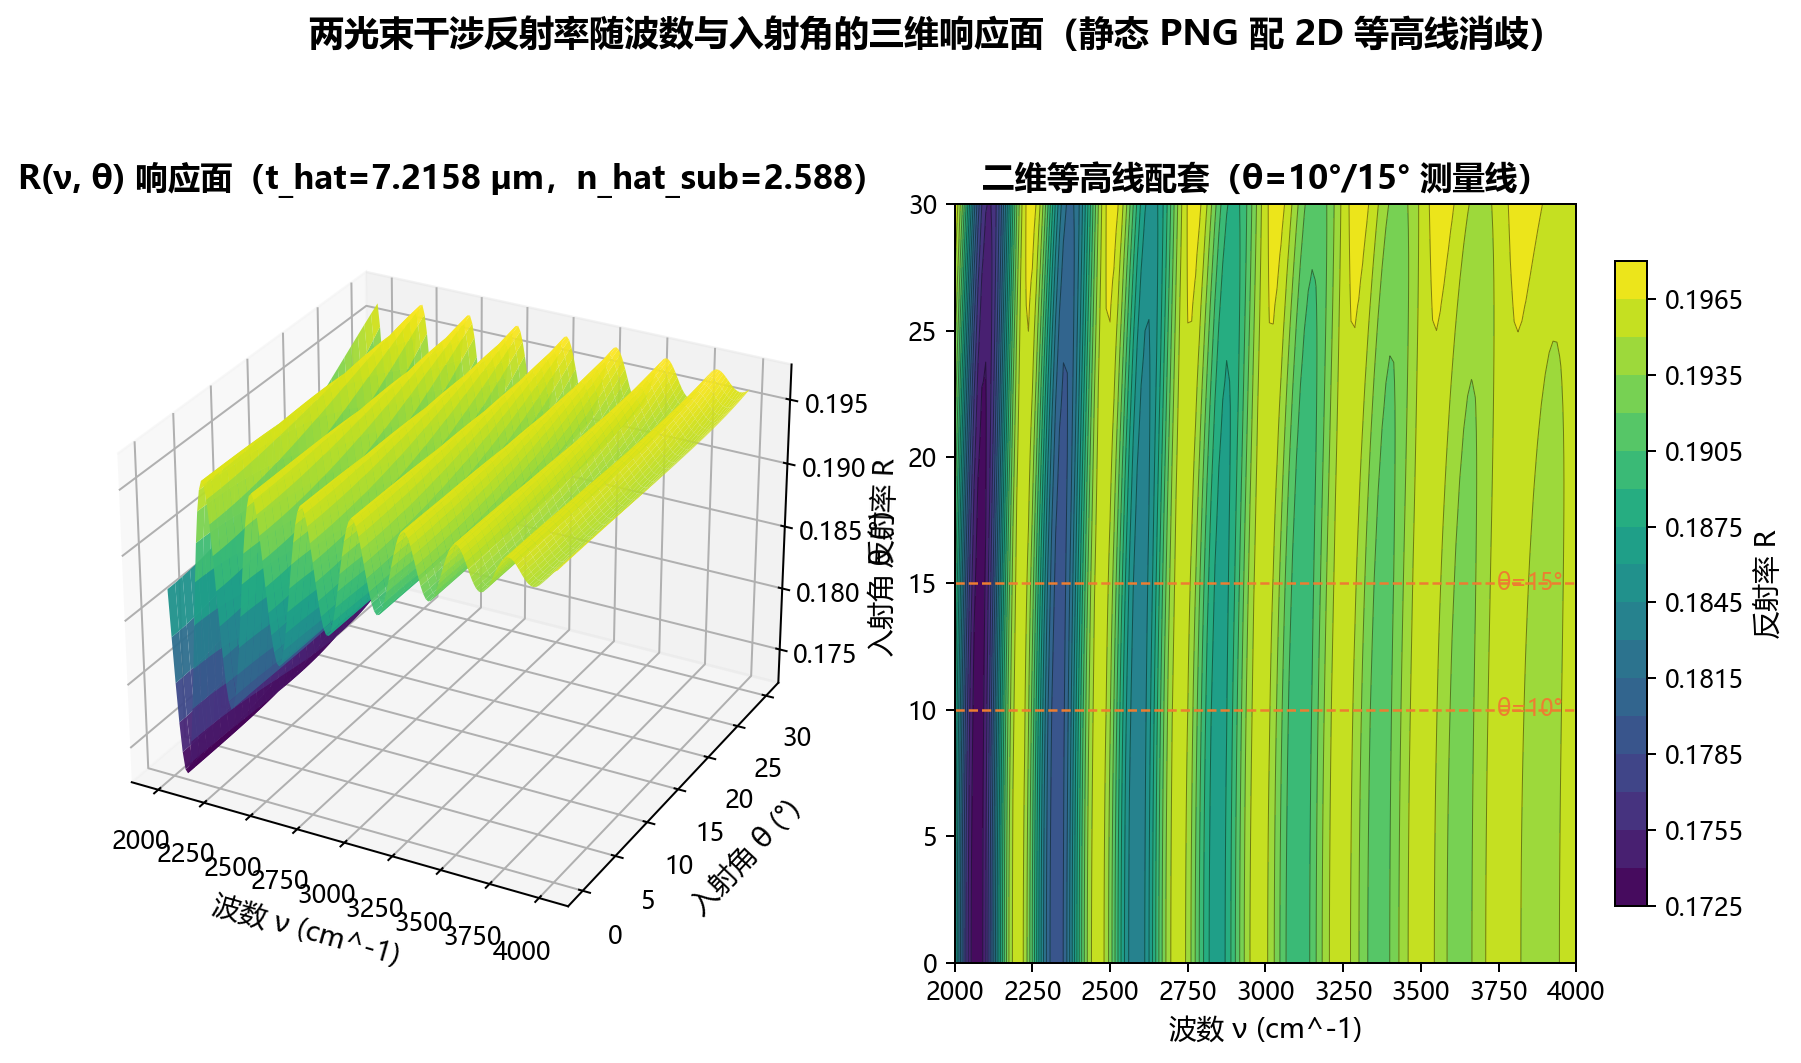
\includegraphics[keepaspectratio,alt={碳化硅反射率的角度---波数响应}]{problems/2025-cumcm-b/prob02/versions/assumption_v001/figures/prob02_fig_response_surface_cfe5827835.png}}

碳化硅反射率的角度---波数响应

图21
给出已估参数下的响应面与等高线，用于观察入射角变化和谱线形状的联系。该模型曲面不替代额外角度的测量验证。

\pandocbounded{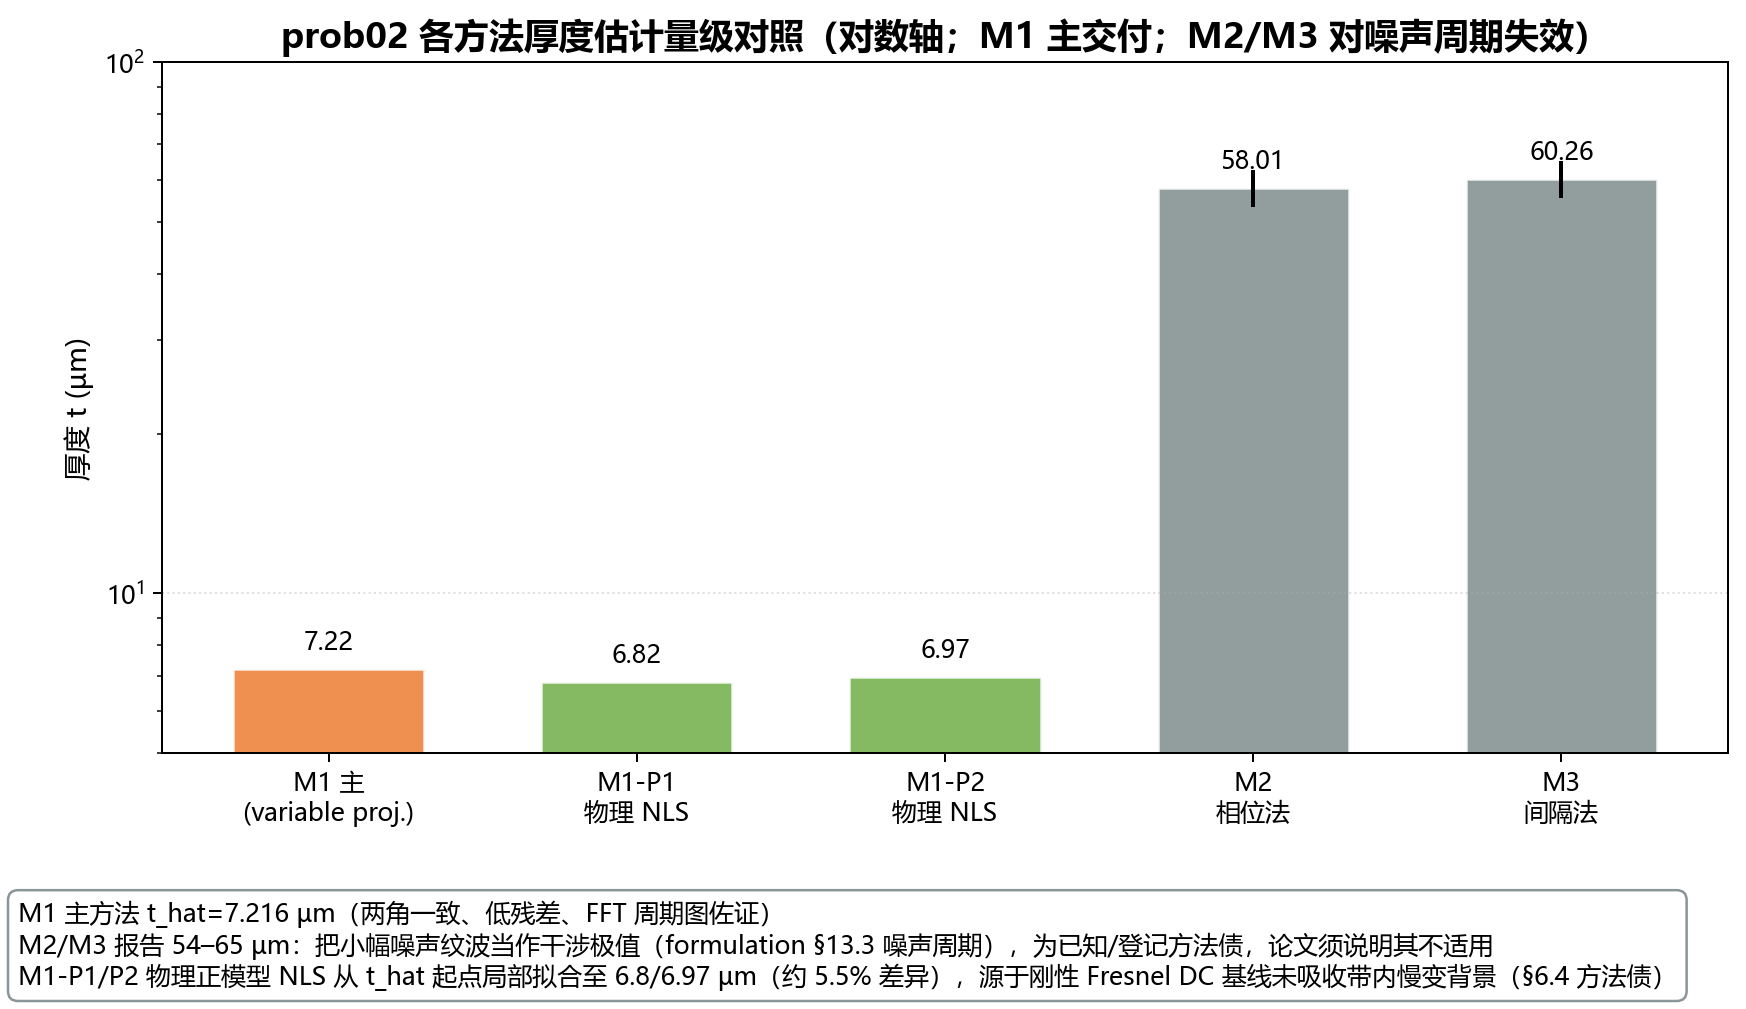
\includegraphics[keepaspectratio,alt={碳化硅不同反演方法的厚度量级}]{problems/2025-cumcm-b/prob02/versions/assumption_v001/figures/prob02_fig_methods_compare_99386076f5.png}}

碳化硅不同反演方法的厚度量级

图22
对比主方法、极值间隔法与物理正模型拟合。约5.5\%的物理拟合差异以及噪声周期导致的错误量级均保留，不用方法平均掩盖模型失配。

问题2 可靠性与结论

采用两角嵌套F检验时，\(F=5.251\)、\(p=0.022\)，在显著性水平0.05下拒绝完全相同的统计假设；与此同时，0.165\%的角度差小于预设2\%工程阈值。本文报告共同厚度作为工程摘要值，并保留独立估计。测量点差异或膜厚梯度是既定解释，不是已经被额外实验确认的因果结论。

带内色散扰动造成0.507\%的厚度变化；异常点处理策略变化在记录精度下为0；主方法对衬底折射率的结构敏感性为0，而物理正模型诊断可出现1.92\%的变化。将不可靠长波区域纳入反演会产生58.42\%的变化，该数字属于谱段选择警示，不应列为``稳健性误差很小''的证据。

\pandocbounded{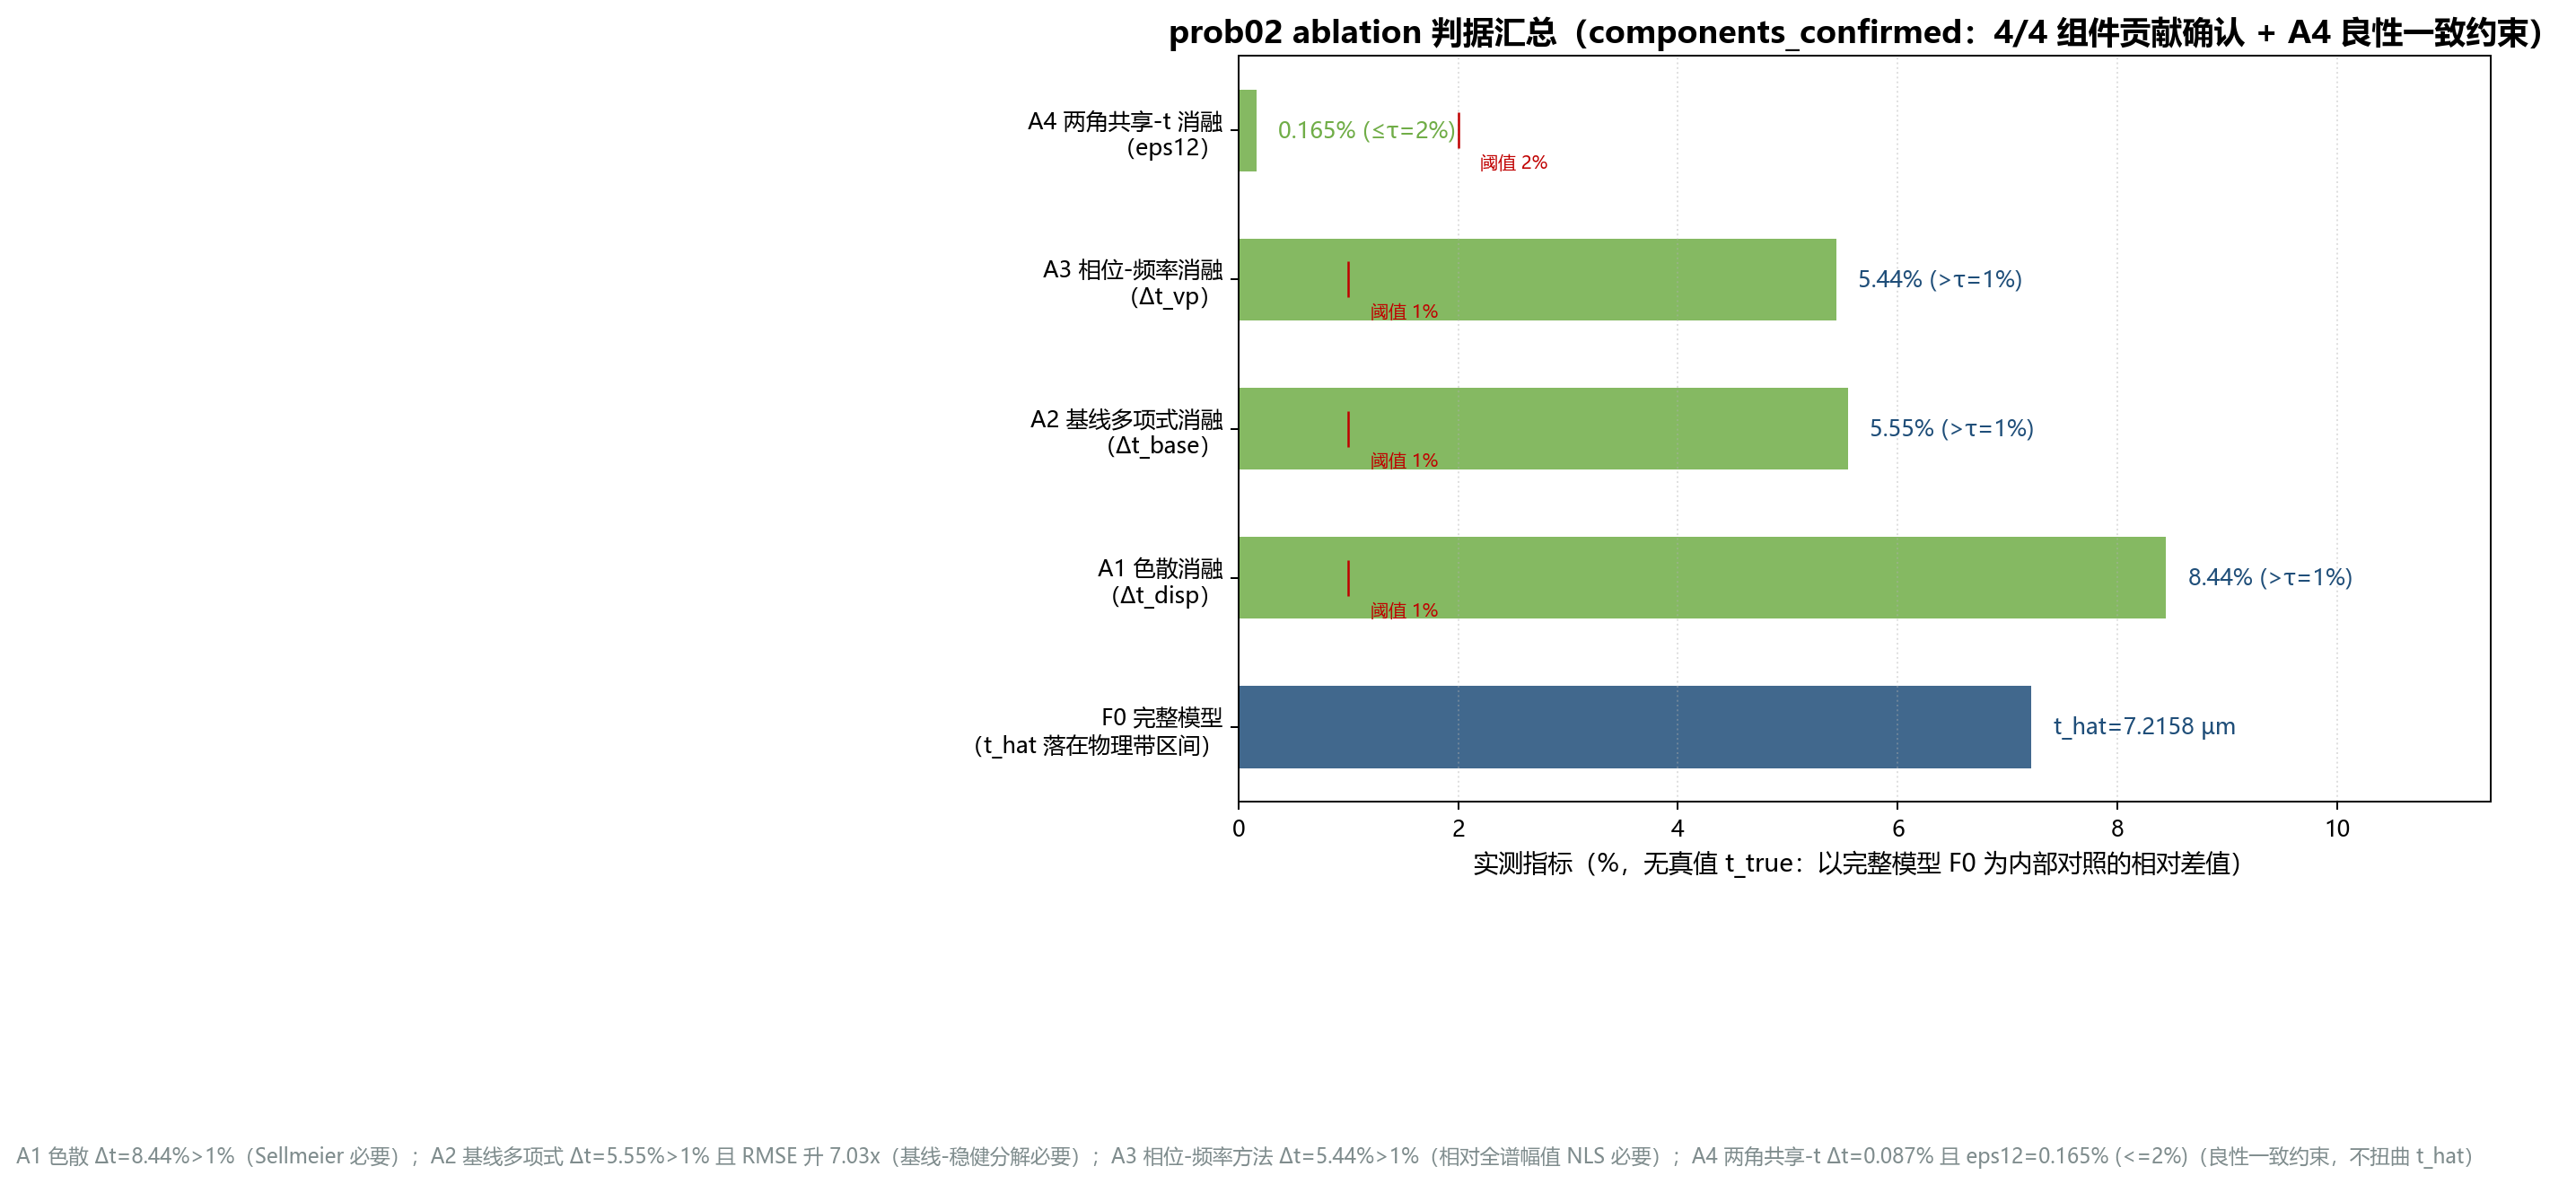
\includegraphics[keepaspectratio,alt={碳化硅模型组成的消融判定}]{problems/2025-cumcm-b/prob02/versions/assumption_v001/figures/prob02_fig_ablation_summary_dcd697b29e.png}}

碳化硅模型组成的消融判定

图23
汇总预先指定的消融实验。删除基线变化会显著影响厚度，说明主方法中的背景与干涉分解不是纯粹的排版性修饰或事后解释。

\pandocbounded{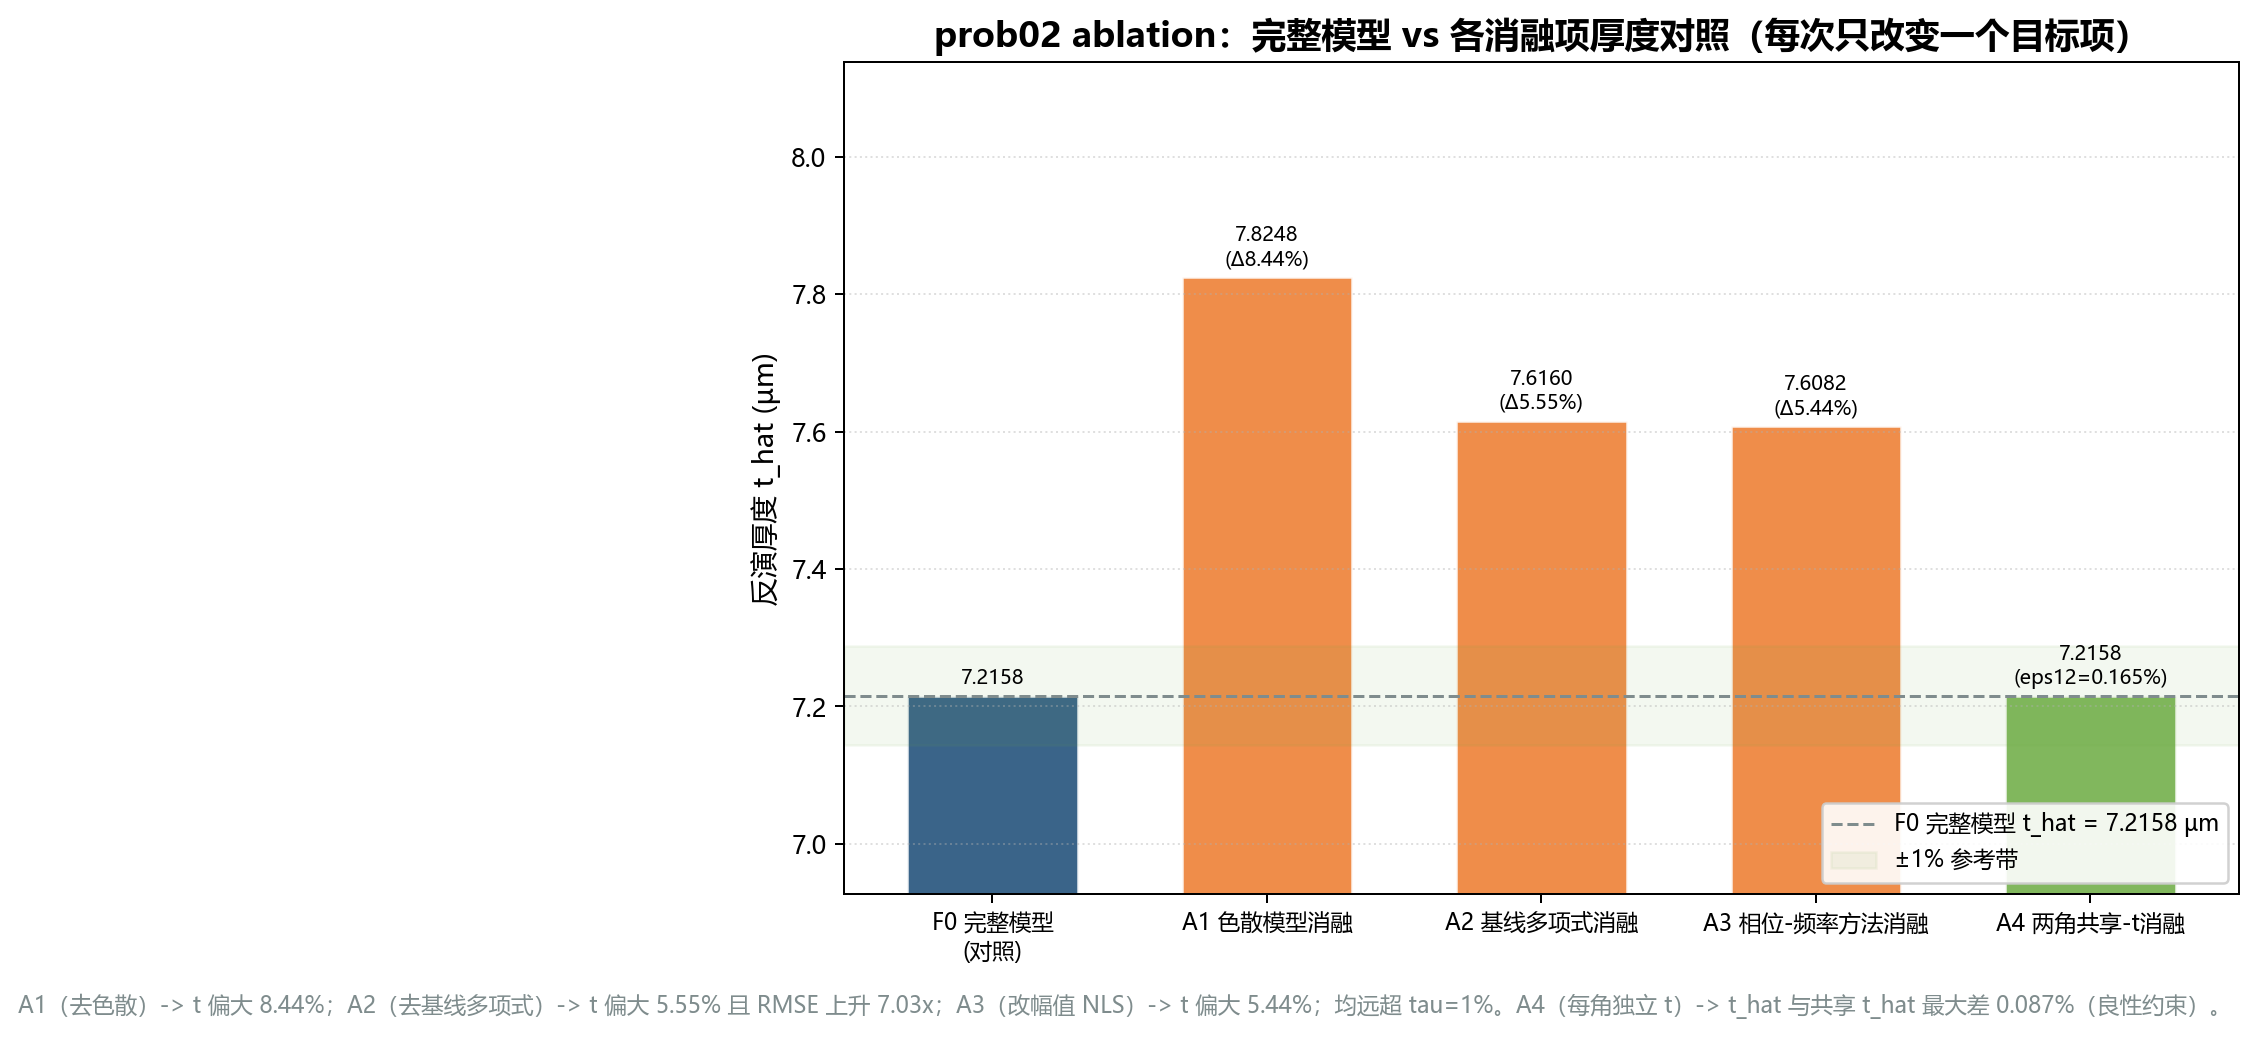
\includegraphics[keepaspectratio,alt={碳化硅消融后的厚度变化}]{problems/2025-cumcm-b/prob02/versions/assumption_v001/figures/prob02_fig_ablation_thickness_d29e3fc1f0.png}}

碳化硅消融后的厚度变化

图24
对比完整模型与不同删减模型的厚度。常数基线方案产生5.55\%的变化，说明基线建模误差可以直接进入厚度估计。

\pandocbounded{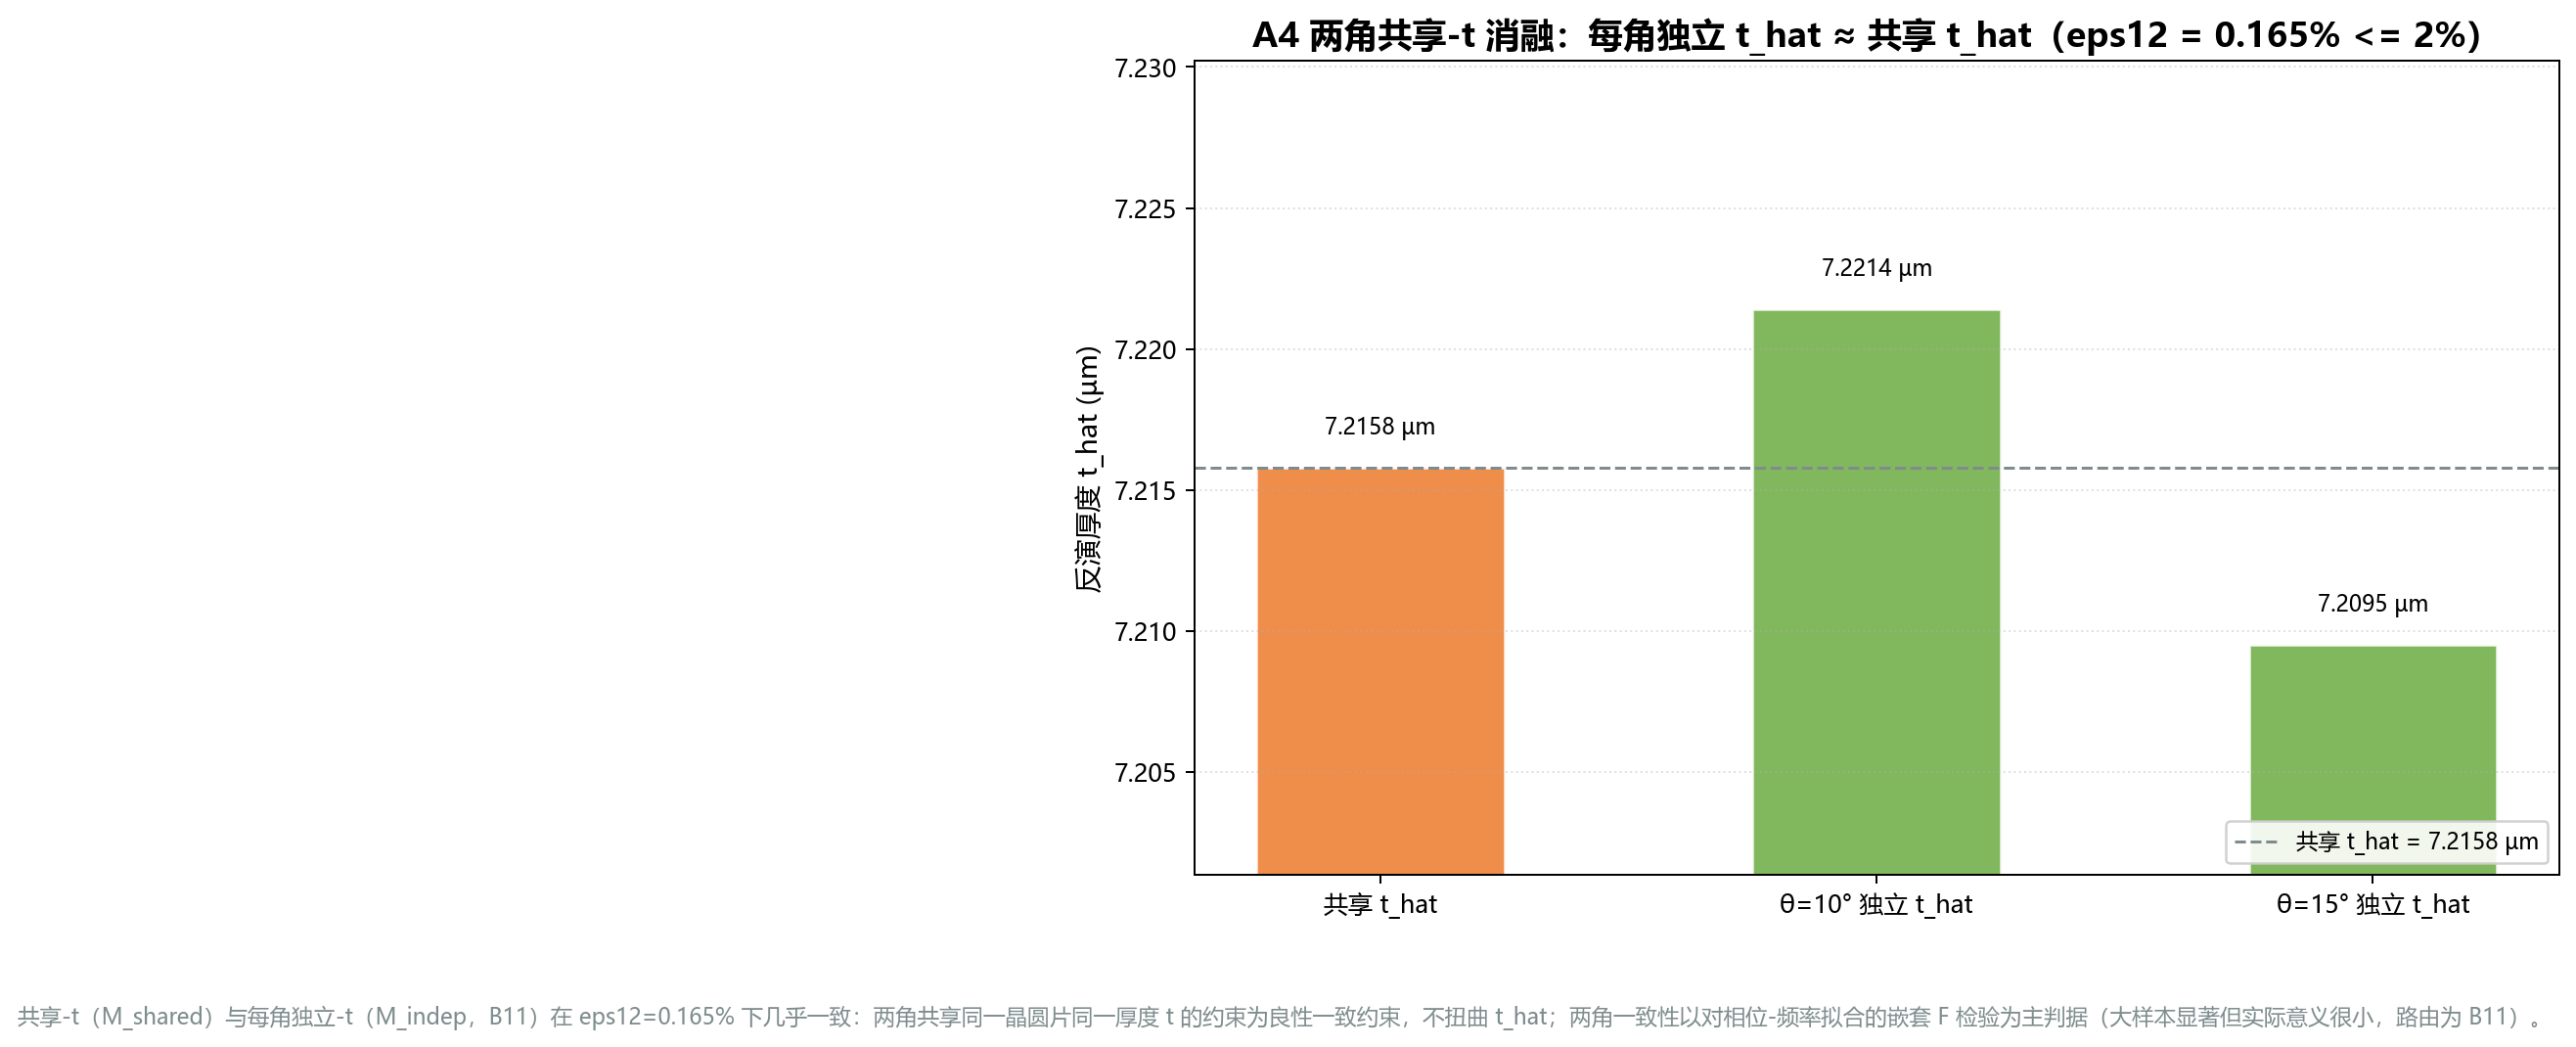
\includegraphics[keepaspectratio,alt={共享厚度约束与独立厚度估计}]{problems/2025-cumcm-b/prob02/versions/assumption_v001/figures/prob02_fig_ablation_shared_t_14e5362fa7.png}}

共享厚度约束与独立厚度估计

图25
展示联合估计与独立角度估计的关系。共享参数利用共同几何信息，而独立估计保留了检验空间不均匀性或测量差异的入口。

去掉慢变基线、改用常数基线后厚度变化5.55\%，拟合误差显著增加；这与刚性物理基线交叉拟合约5.5\%的厚度差异方向相符。细密噪声峰导致的54---65
μm量级也不进入主结果。当前7.2158
μm的结论依赖既定色散和相位分解，不宣称所有候选模型一致。

衬底折射率仍为幅度弱辨识值；SiC长波端色散、部分材料文献全文、未实施的重采样置信分析都是尚未完成的验证。背景阶数扰动与主结果并非完全重合，不能以较窄的条件置信区间掩盖模型选择不确定性。本文不新增这些试验，也不把``无需重新修订模型''改写为``没有剩余误差''。

问题3 多光束条件及硅厚度反演

问题3 问题分析与Airy模型

在平行界面上，各次往返的复振幅形成几何级数。设界面振幅反射系数为
\(r_{01}\)、\(r_{12}\)，则

\[r=\frac{r_{01}+r_{12}e^{i\delta}}{1+r_{01}r_{12}e^{i\delta}},\qquad R_{\mathrm{Airy}}=|r|^2.\]

对透明介质，在一致处理反射相位的约定下可写为

\[R_{\mathrm{Airy}}=\frac{R_{01}+R_{12}+2\sqrt{R_{01}R_{12}}\cos\delta}
{1+R_{01}R_{12}+2\sqrt{R_{01}R_{12}}\cos\delta}.\]

多次反射与近似平行板的有关研究构成这一模型的背景
{[}28{]}、{[}29{]}、{[}30{]}、{[}31{]}、{[}32{]}。多光束的``存在''与``对厚度估计有显著影响''是两个不同问题。

问题3 必要条件与厚度影响

高阶反射形成可观察干涉，需要反射后的幅度未过快衰减、相干长度足够、界面平行性与光束重叠满足要求，并且吸收未将往返光束显著衰减。界面反射率的几何平均及精细度参数记为

\[\bar R=\sqrt{R_{01}R_{12}},\qquad
\mathcal F=\frac{\pi\sqrt{\bar R}}{1-\bar R}.\]

本文按原方案将 \(\bar R\le0.05\)
作为量级诊断，并结合Airy相对物理两光束基线的残差改善是否超过10\%判定是否需要修正。二者是当前分析的预设阈值，不是适用于所有仪器和晶圆的自然常数。

令
\(A=R_{01}+R_{12}\)、\(B=2\sqrt{R_{01}R_{12}}\)、\(C=1+R_{01}R_{12}\)。当比较相位变化时把界面系数固定，有

\[\frac{dR_{\mathrm{Airy}}}{d\delta}
=\frac{B(A-C)\sin\delta}{(C+B\cos\delta)^2}.\]

因此在非退化的透明平板情形，相位极值仍对应
\(\delta=m\pi\)。这一结论解释了高阶反射主要改变峰形而不改变基本相位周期；它不是对吸收介质、明显色散的振幅变化或有限噪声拟合中厚度偏差严格为零的断言。

问题3 硅数据算法与厚度结果

硅采用自身材料色散关系
{[}12{]}、{[}13{]}、{[}14{]}，其主反演带内色散较弱。计算仍用基线---干涉分解与一维变量投影，透明谱段选为
\([2000,4000]\ \mathrm{cm}^{-1}\)。相位函数保留斜入射几何，避免用半周期或材料错误引入厚度倍数偏差。

硅外延层厚度与条件不确定性

\begin{longtable}[]{@{}lll@{}}
\toprule\noalign{}
估计对象 & 厚度/μm & 辅助指标 \\
\midrule\noalign{}
\endhead
\bottomrule\noalign{}
\endlastfoot
两角共享 & 3.4477 & 95\%轮廓区间相对半宽约0.134\% \\
10°独立估计 & 3.4507 & 与另一角度合算相对差0.130\% \\
15°独立估计 & 3.4463 & 当前共同厚度的角度对照 \\
\end{longtable}

\pandocbounded{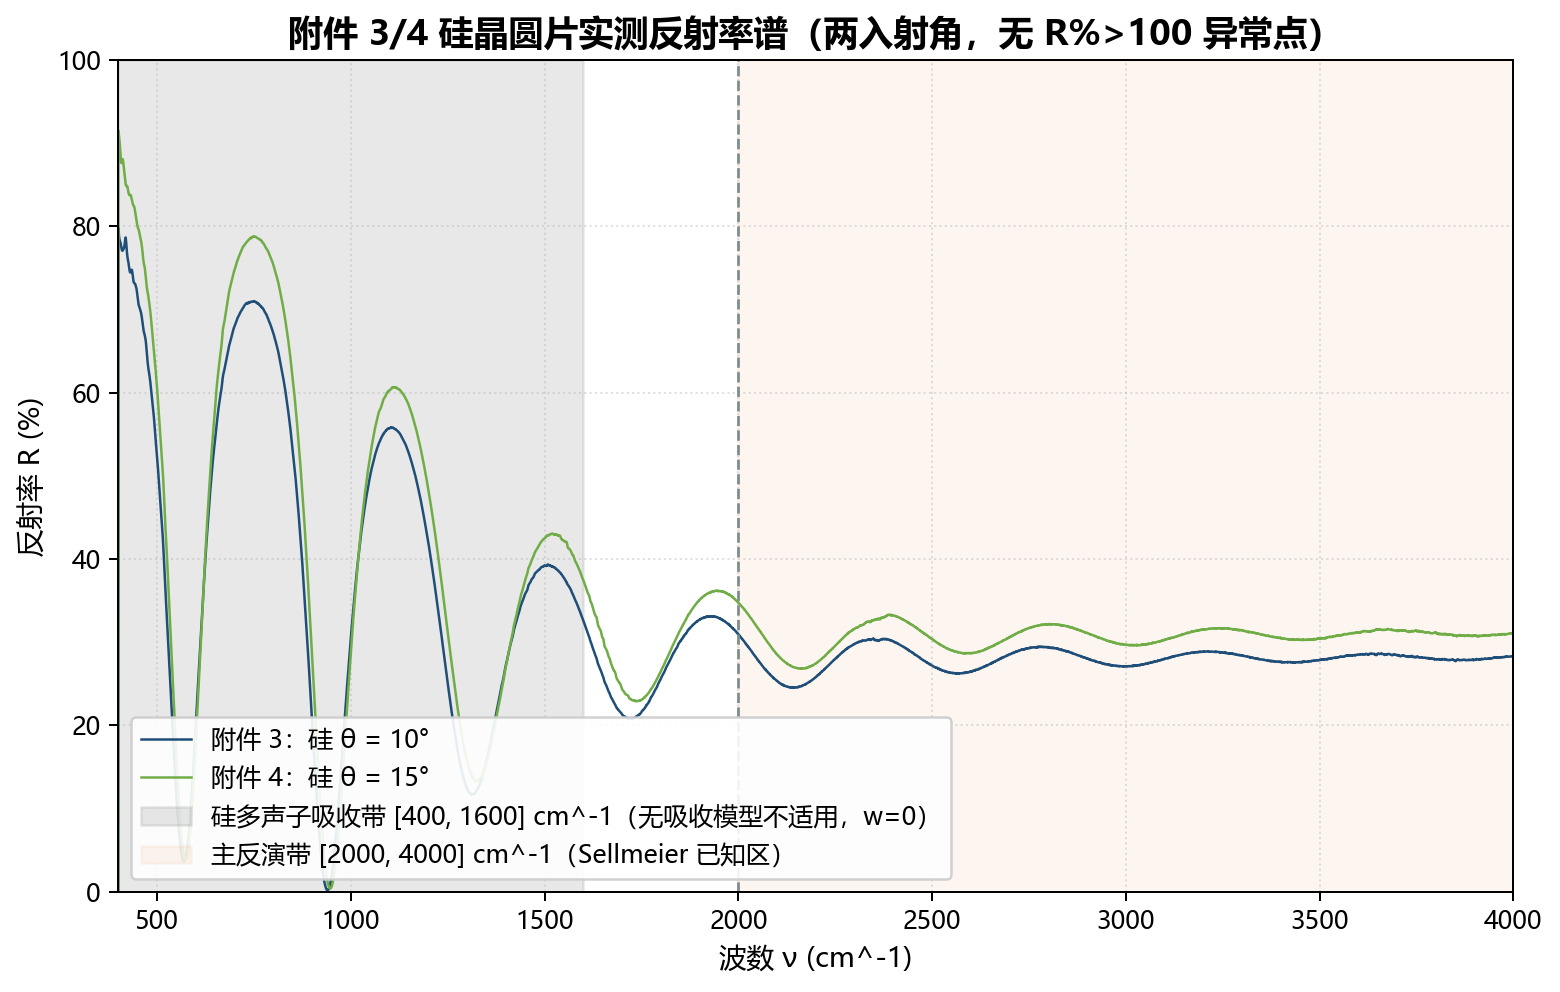
\includegraphics[keepaspectratio,alt={硅两入射角实测反射率谱}]{problems/2025-cumcm-b/prob03/versions/assumption_v001/figures/prob03_fig_reflectance_spectrum_41a3800f70.png}}

硅两入射角实测反射率谱

图26
给出附件3、4的数据。与碳化硅相比，所用透明谱段和折射率规律不同，因此不能直接沿用碳化硅的材料参数。

\pandocbounded{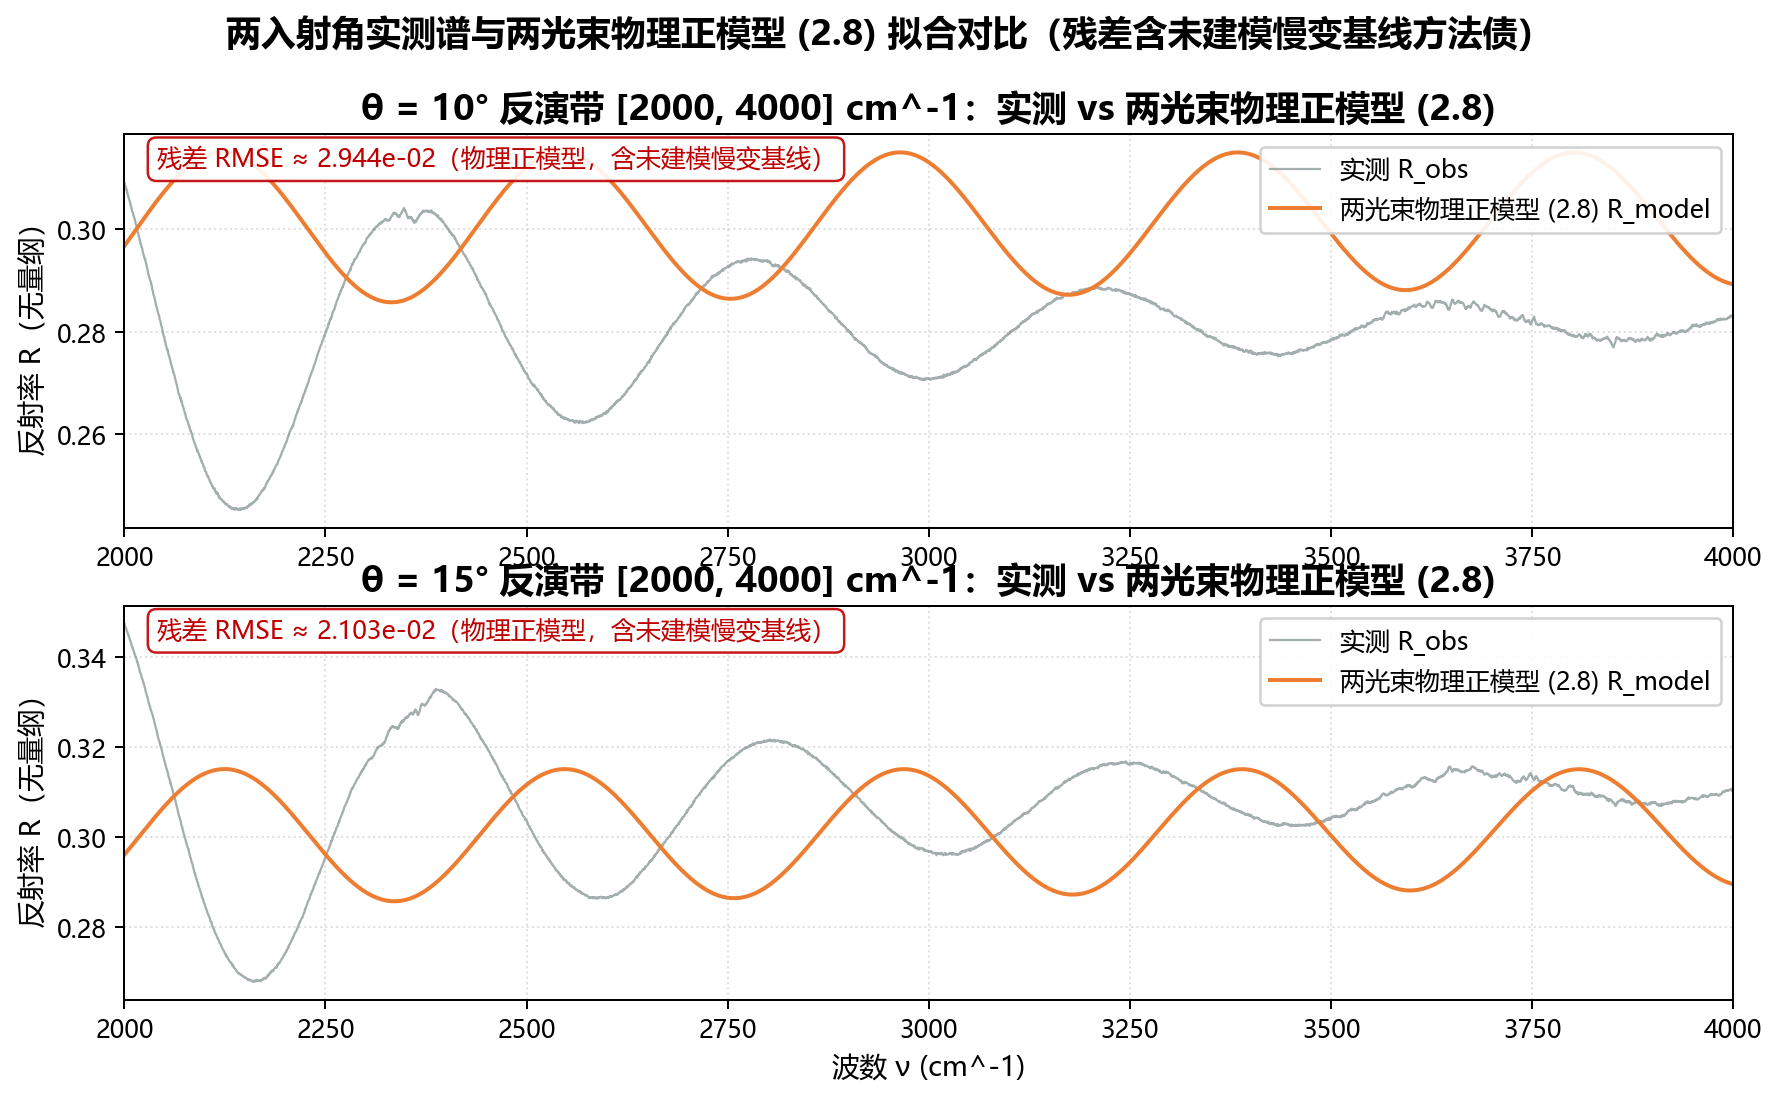
\includegraphics[keepaspectratio,alt={硅实测谱与物理两光束诊断拟合}]{problems/2025-cumcm-b/prob03/versions/assumption_v001/figures/prob03_fig_model_fit_3e94d2fac7.png}}

硅实测谱与物理两光束诊断拟合

图27
对比硅测量谱与物理正模型，用于观察幅度和基线失配。多光束残差改善以这一物理基线为比较对象，不与变量投影的残差混用。

\pandocbounded{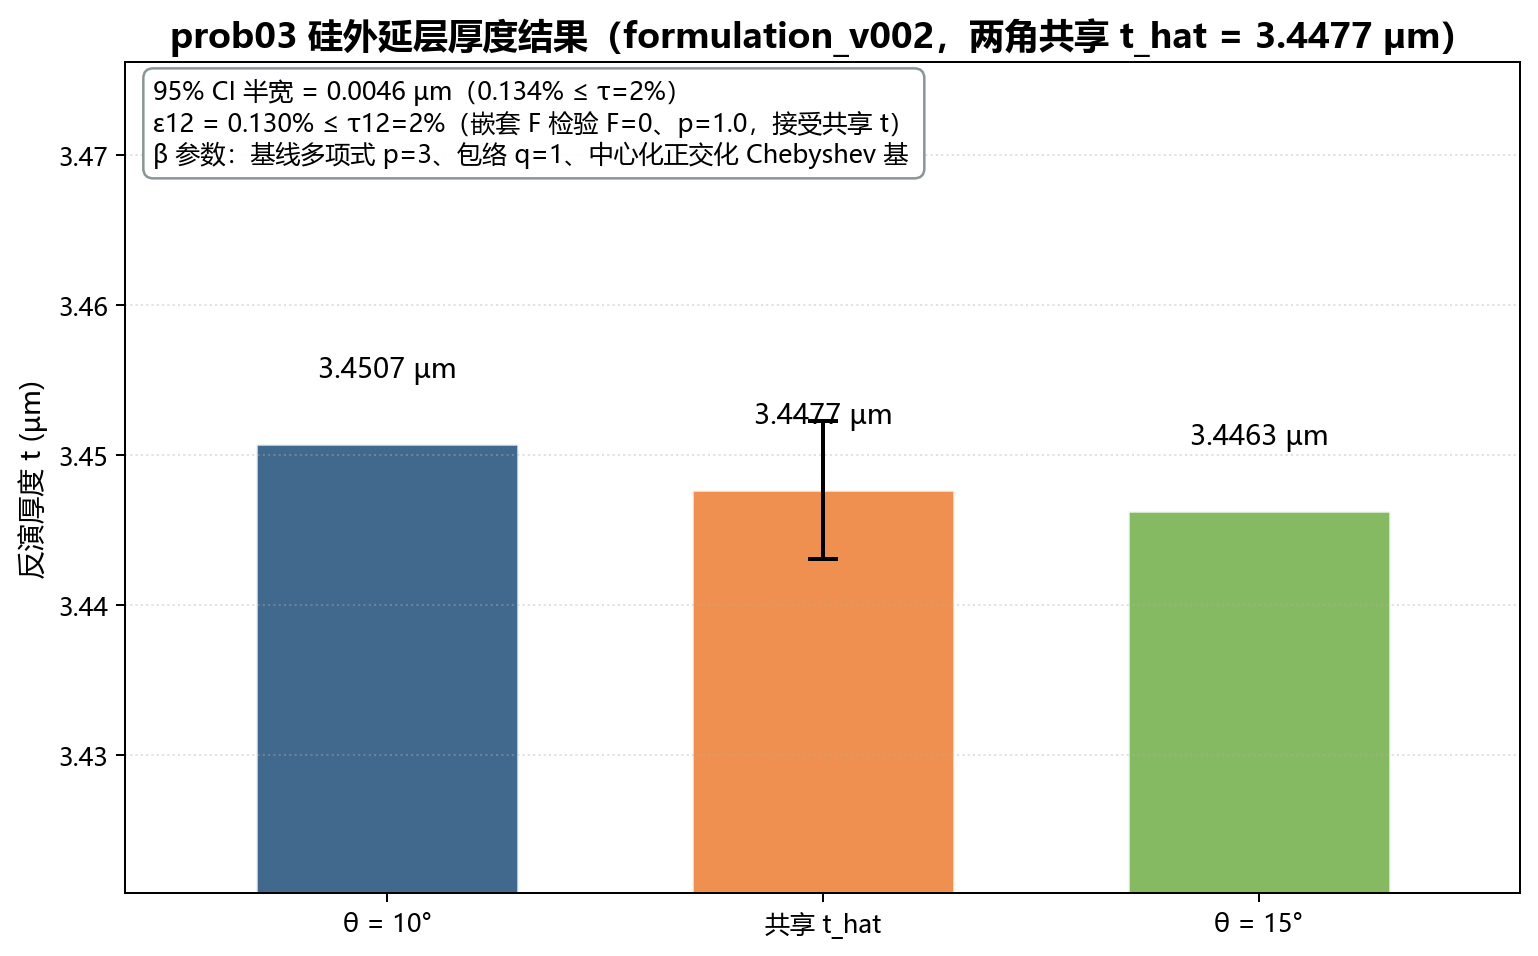
\includegraphics[keepaspectratio,alt={硅共享厚度与分角度厚度估计}]{problems/2025-cumcm-b/prob03/versions/assumption_v001/figures/prob03_fig_thickness_estimate_59f1546ed7.png}}

硅共享厚度与分角度厚度估计

图28 展示共享厚度3.4477 μm及两角3.4507、3.4463
μm。0.130\%的角度相对差支持在现有工程容差下报告共同厚度。

\pandocbounded{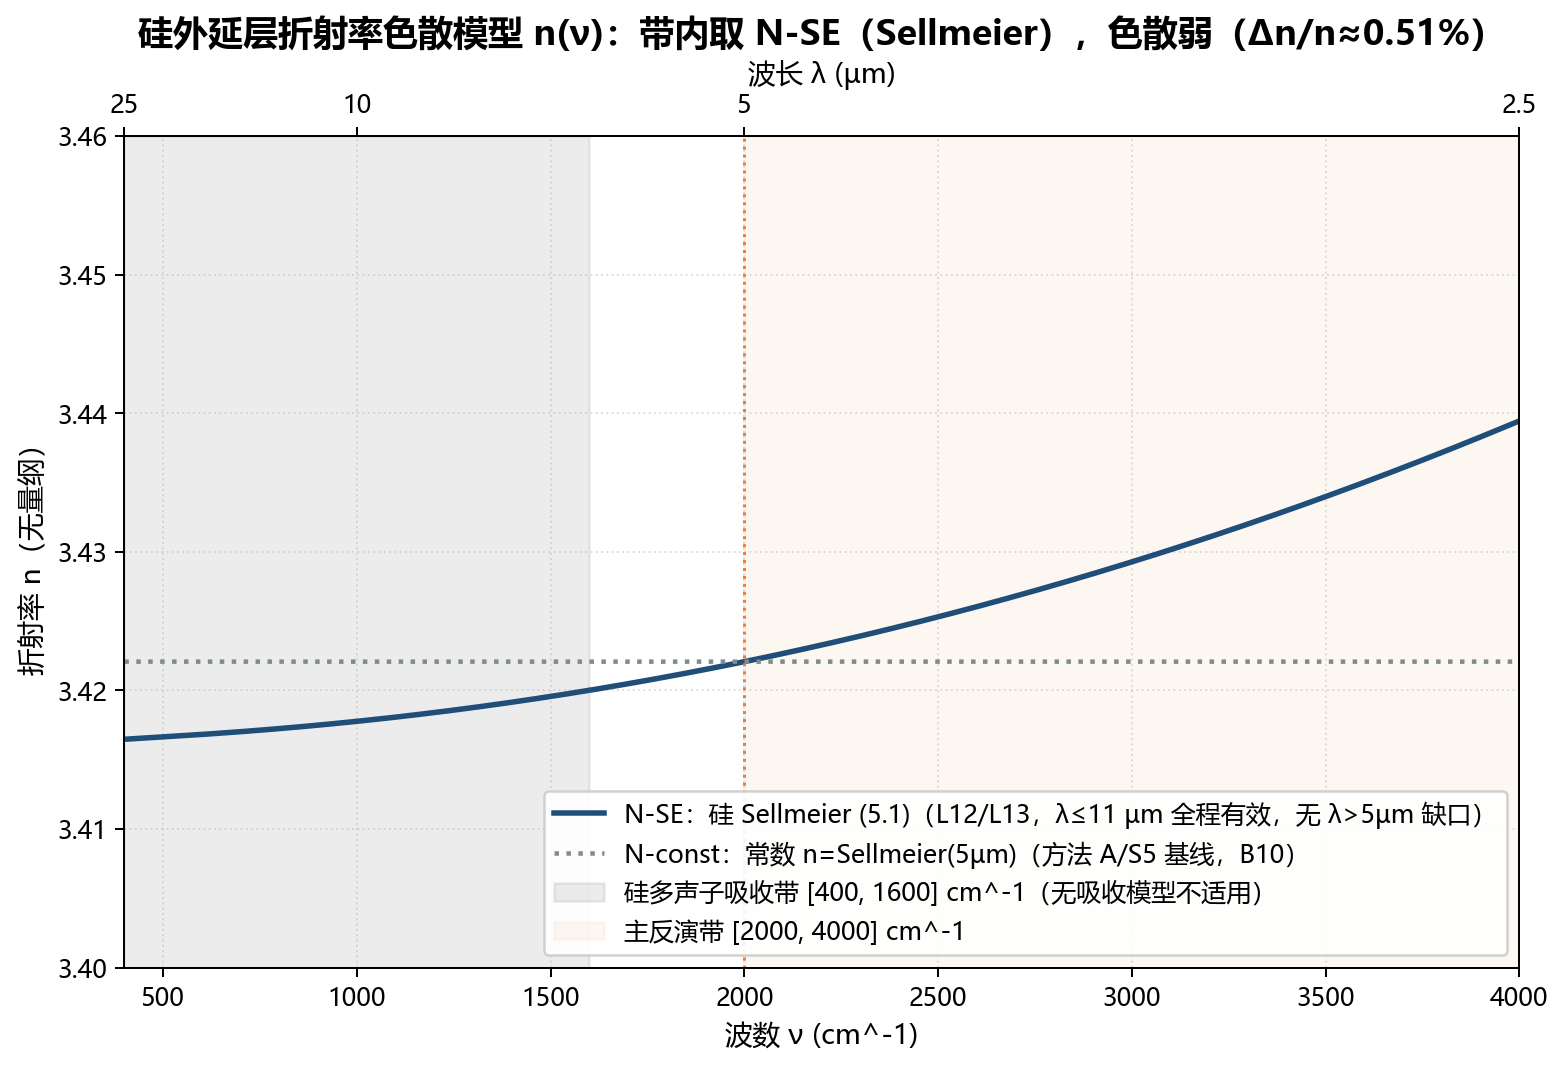
\includegraphics[keepaspectratio,alt={硅主反演谱段内的弱色散}]{problems/2025-cumcm-b/prob03/versions/assumption_v001/figures/prob03_fig_dispersion_curve_aac3dcebea.png}}

硅主反演谱段内的弱色散

图29
给出硅折射率在分析波段内的缓慢变化。弱色散降低了常数折射率近似的影响，也使某些周期候选更接近，故仍须检查整个目标函数。

\pandocbounded{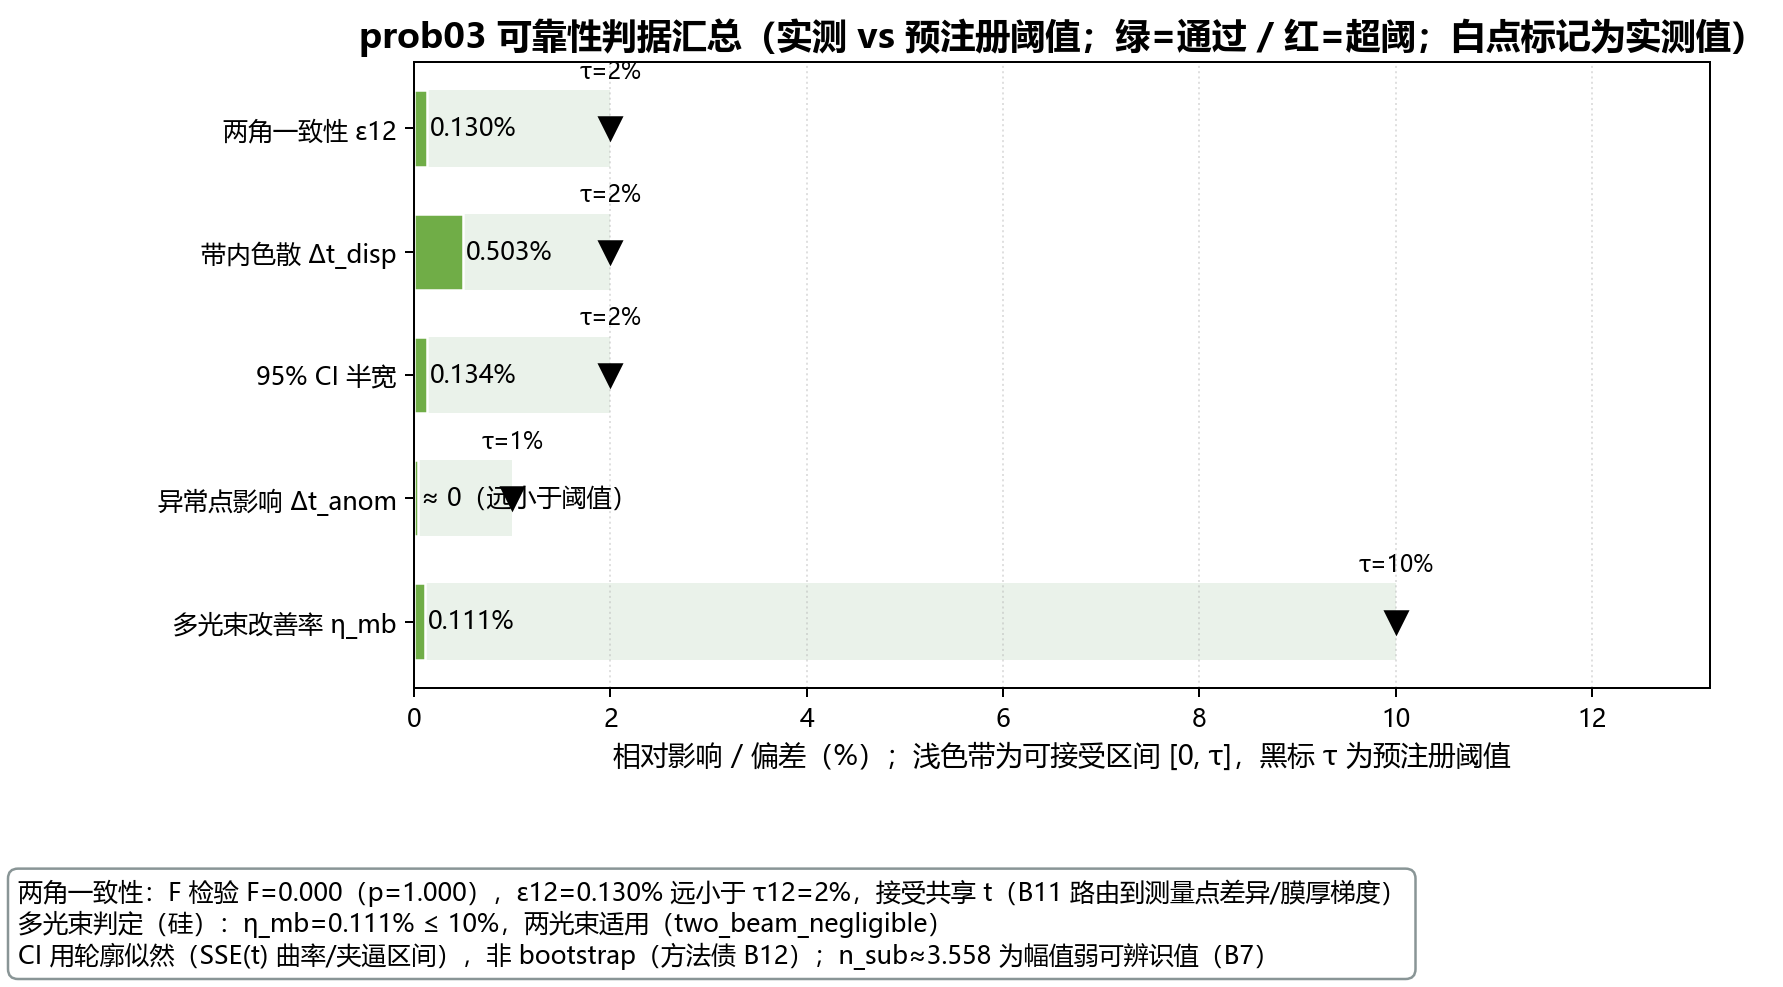
\includegraphics[keepaspectratio,alt={硅可靠性指标与报告边界}]{problems/2025-cumcm-b/prob03/versions/assumption_v001/figures/prob03_fig_reliability_summary_50b4f34a17.png}}

硅可靠性指标与报告边界

图30
汇总色散、区间、异常点和多光束等指标。接近1的次小候选比值属于需要披露的辨识边界，不能说成具有很大的唯一性裕度。

\pandocbounded{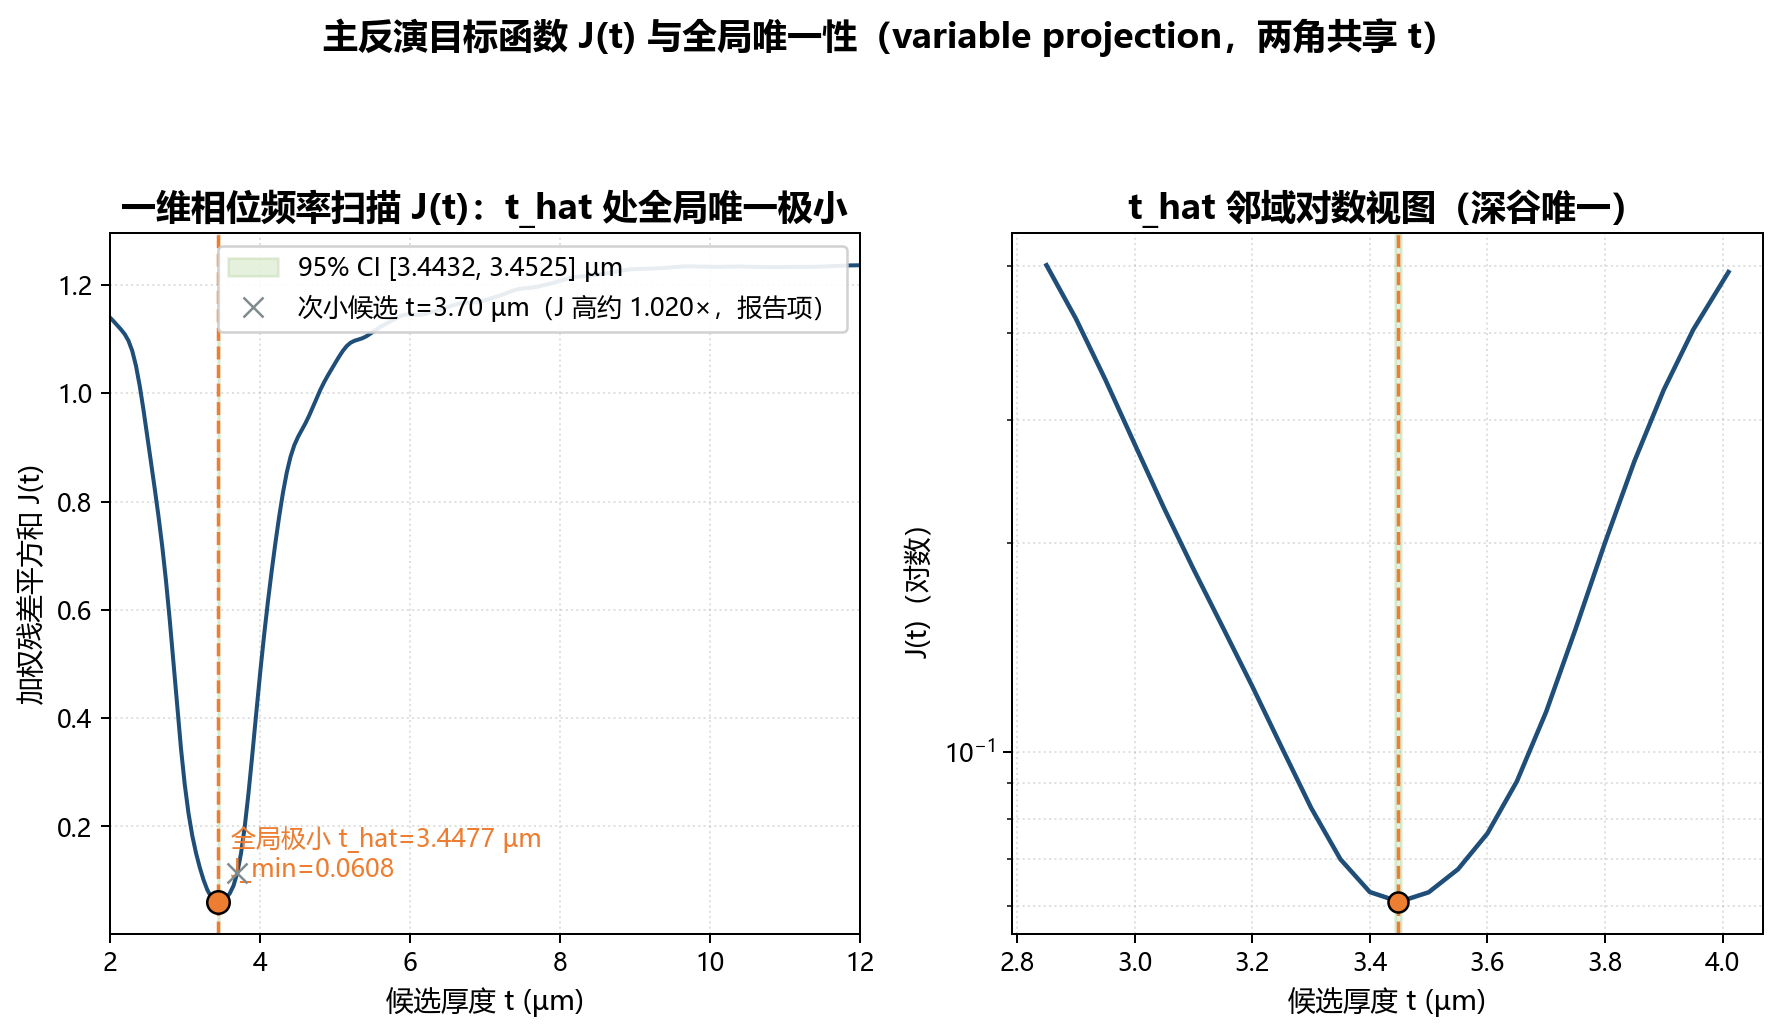
\includegraphics[keepaspectratio,alt={硅厚度目标函数与邻近候选}]{problems/2025-cumcm-b/prob03/versions/assumption_v001/figures/prob03_fig_variable_projection_jcurve_4b30b360a4.png}}

硅厚度目标函数与邻近候选

图31 显示约3.45
μm附近的最小值和其他周期候选。次小候选比值约1.020，结论依赖当前搜索范围、色散设定及预设判据。

\pandocbounded{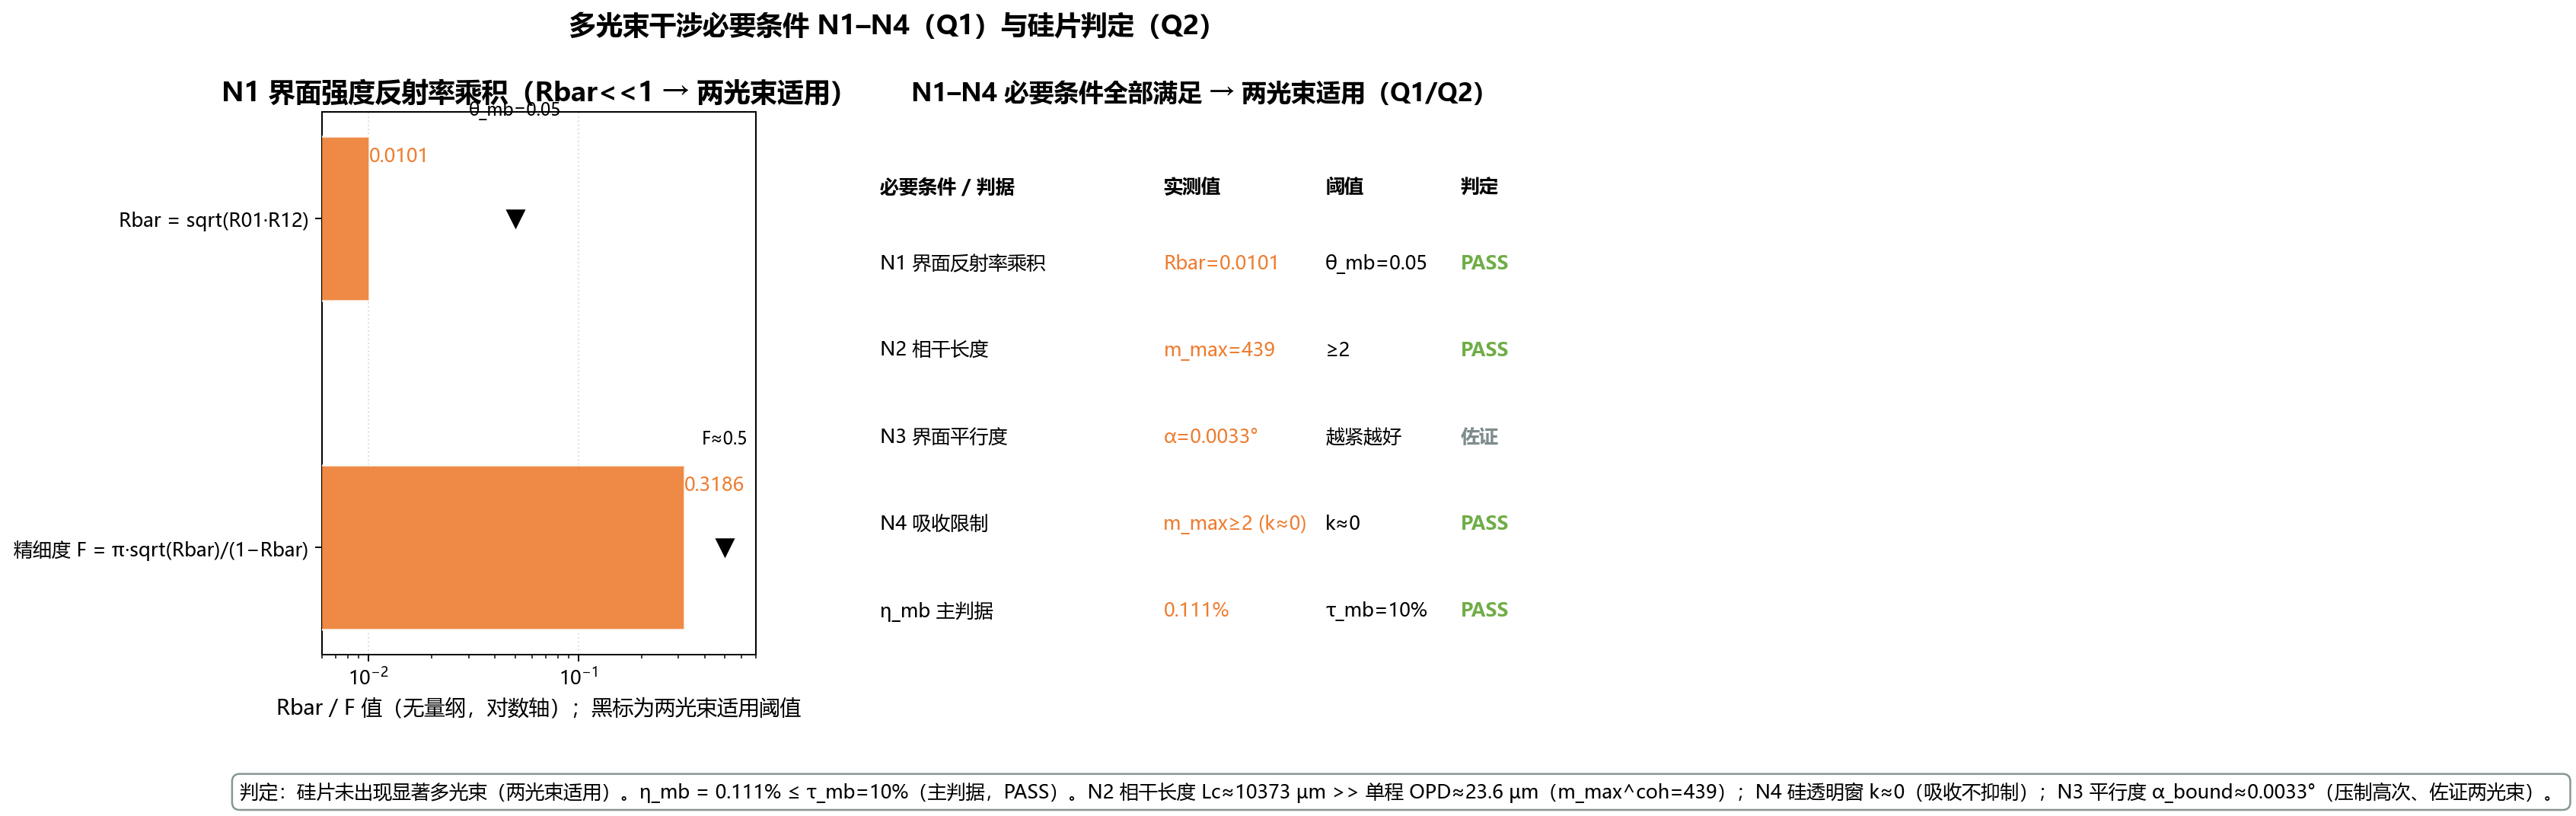
\includegraphics[keepaspectratio,alt={多光束相干、几何与反射率条件}]{problems/2025-cumcm-b/prob03/versions/assumption_v001/figures/prob03_fig_mb_conditions_9571a5012b.png}}

多光束相干、几何与反射率条件

图32
汇总高阶反射能否形成可观测干涉的必要因素。相干性与平行性允许高阶束叠加，但是否需要修正厚度，还要看界面反射率及残差改善。

\pandocbounded{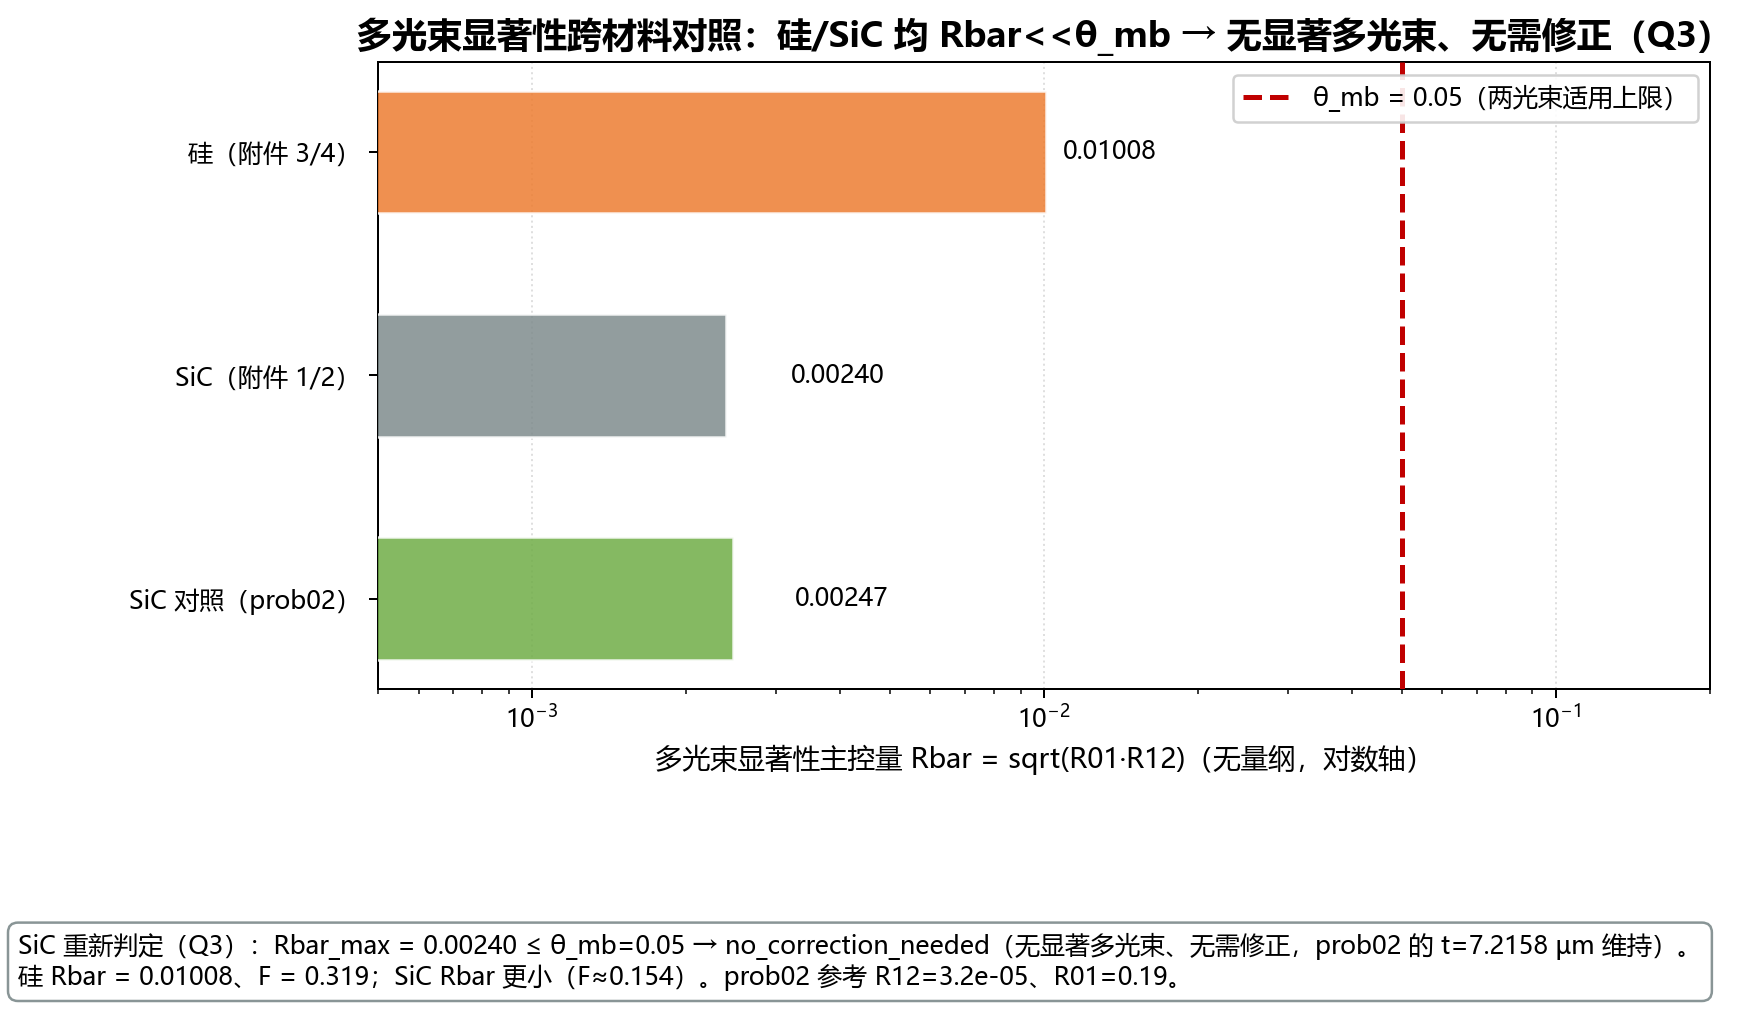
\includegraphics[keepaspectratio,alt={硅与碳化硅的多光束显著性对照}]{problems/2025-cumcm-b/prob03/versions/assumption_v001/figures/prob03_fig_sic_multibeam_recheck_4cbb136f9c.png}}

硅与碳化硅的多光束显著性对照

图33
对比两材料的界面反射率几何平均。硅约0.0101、碳化硅约0.0024，均低于预设量级阈值；不据此宣称高阶反射在物理上完全不存在。

\pandocbounded{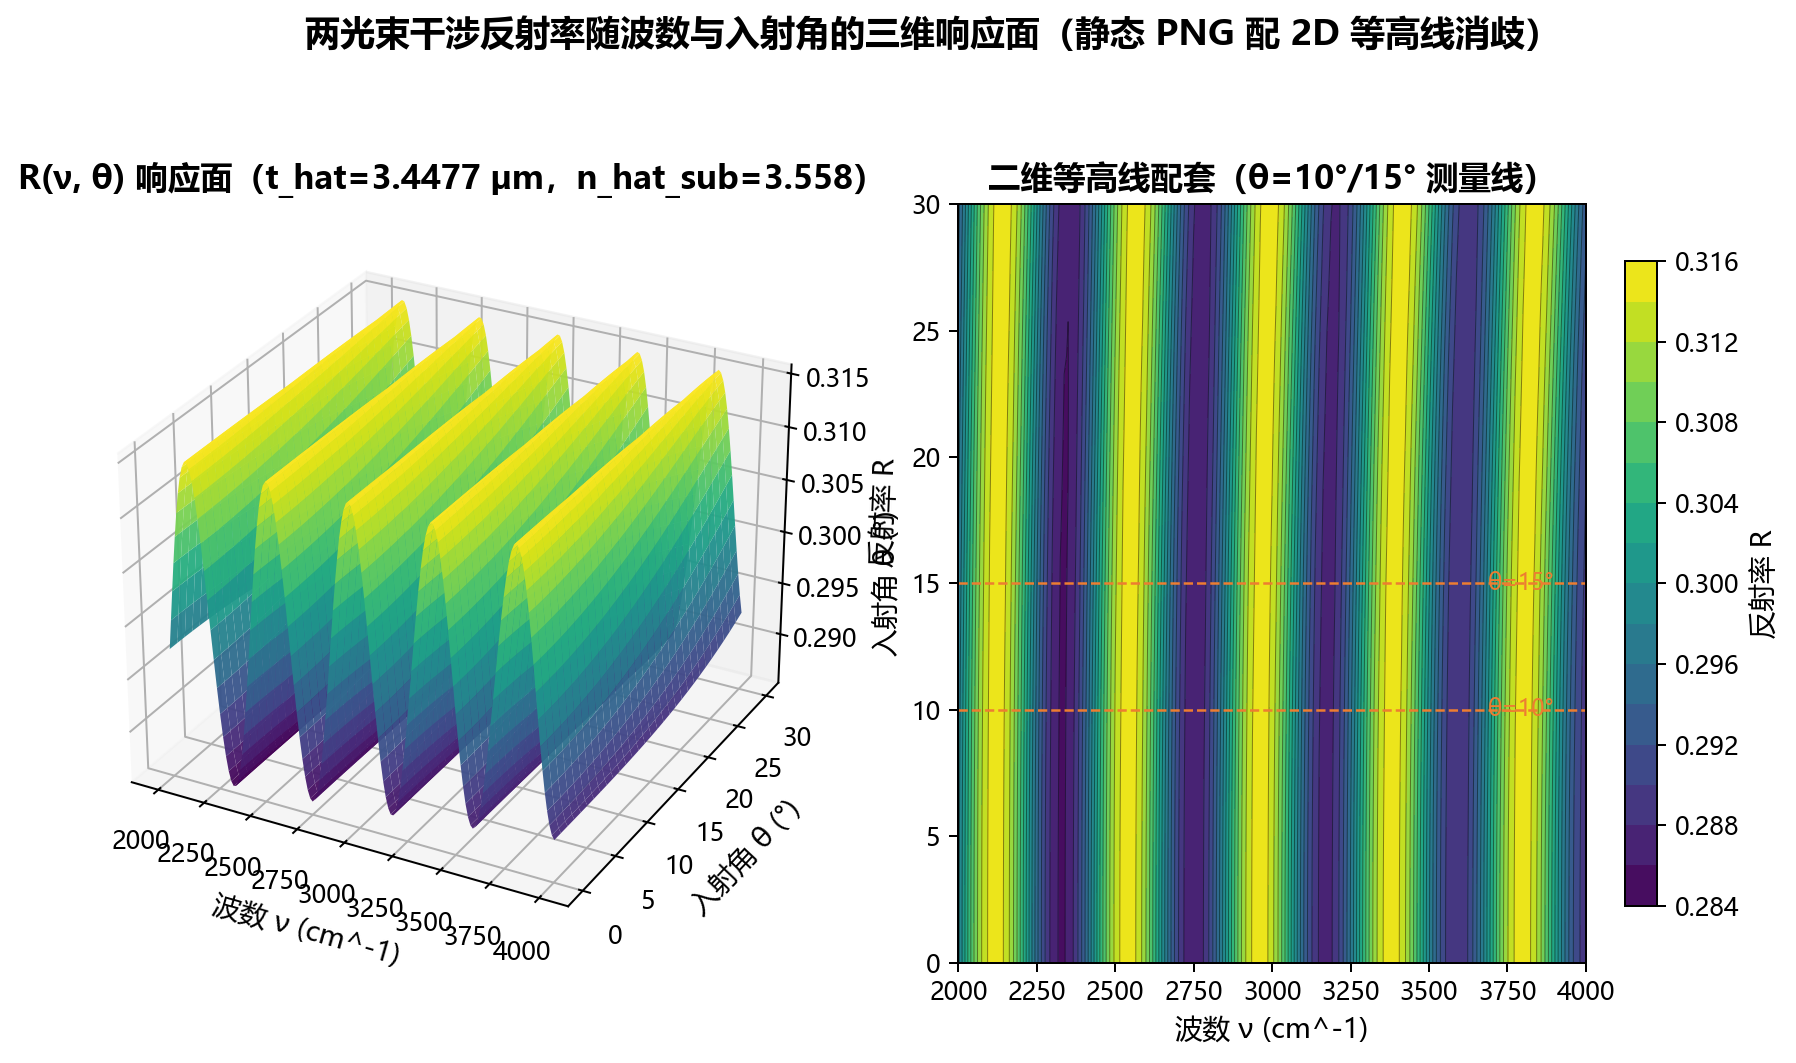
\includegraphics[keepaspectratio,alt={硅反射率的角度---波数响应}]{problems/2025-cumcm-b/prob03/versions/assumption_v001/figures/prob03_fig_response_surface_06cfec9b1e.png}}

硅反射率的角度---波数响应

图34
展示硅已估参数下的连续响应。其作用是解释模型行为，不能据图外推到强吸收区域或未经验证的掺杂范围。

\pandocbounded{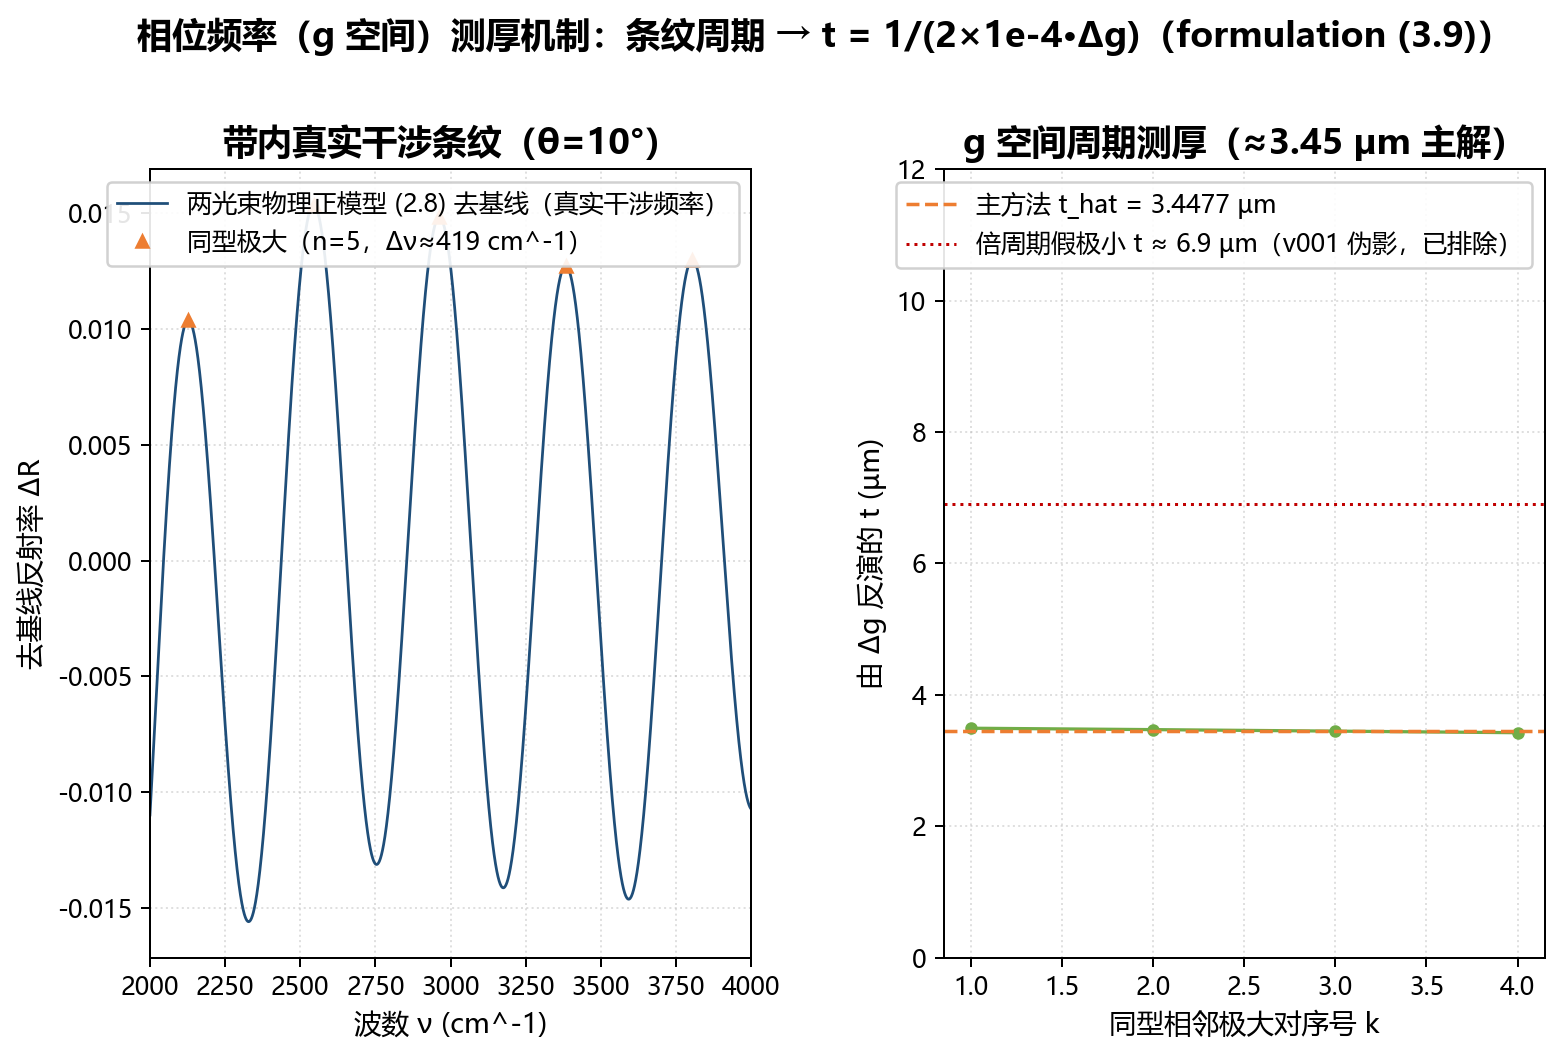
\includegraphics[keepaspectratio,alt={硅相位函数坐标中的干涉条纹}]{problems/2025-cumcm-b/prob03/versions/assumption_v001/figures/prob03_fig_phase_freq_gspace_a936624612.png}}

硅相位函数坐标中的干涉条纹

图35
给出条纹计数与相位积累关系，帮助区分完整周期与半周期，避免厚度出现倍数误判。

问题3 多光束判定与碳化硅回代

硅的 \(\bar R\approx0.0101\)，对应
\(\mathcal F\approx0.319\)。物理基线下两角的Airy残差改善分别约0.038\%和0.111\%，最大值仍明显小于10\%的预设阈值。碳化硅的
\(\bar R\approx0.0024\) 更小，故现有数据不要求在7.2158
μm主结果之外另给一个无依据的``修正厚度''。这里的结论是高阶贡献不足以触发当前判据，而非证明不存在多次反射。

Airy改善率使用刚性Fresnel背景的物理两光束模型作分母；变量投影允许基线变化，两者残差不可直接混比。硅加入高阶谐波后的厚度变化为0.300\%，也说明实际拟合不是严格零影响。

\pandocbounded{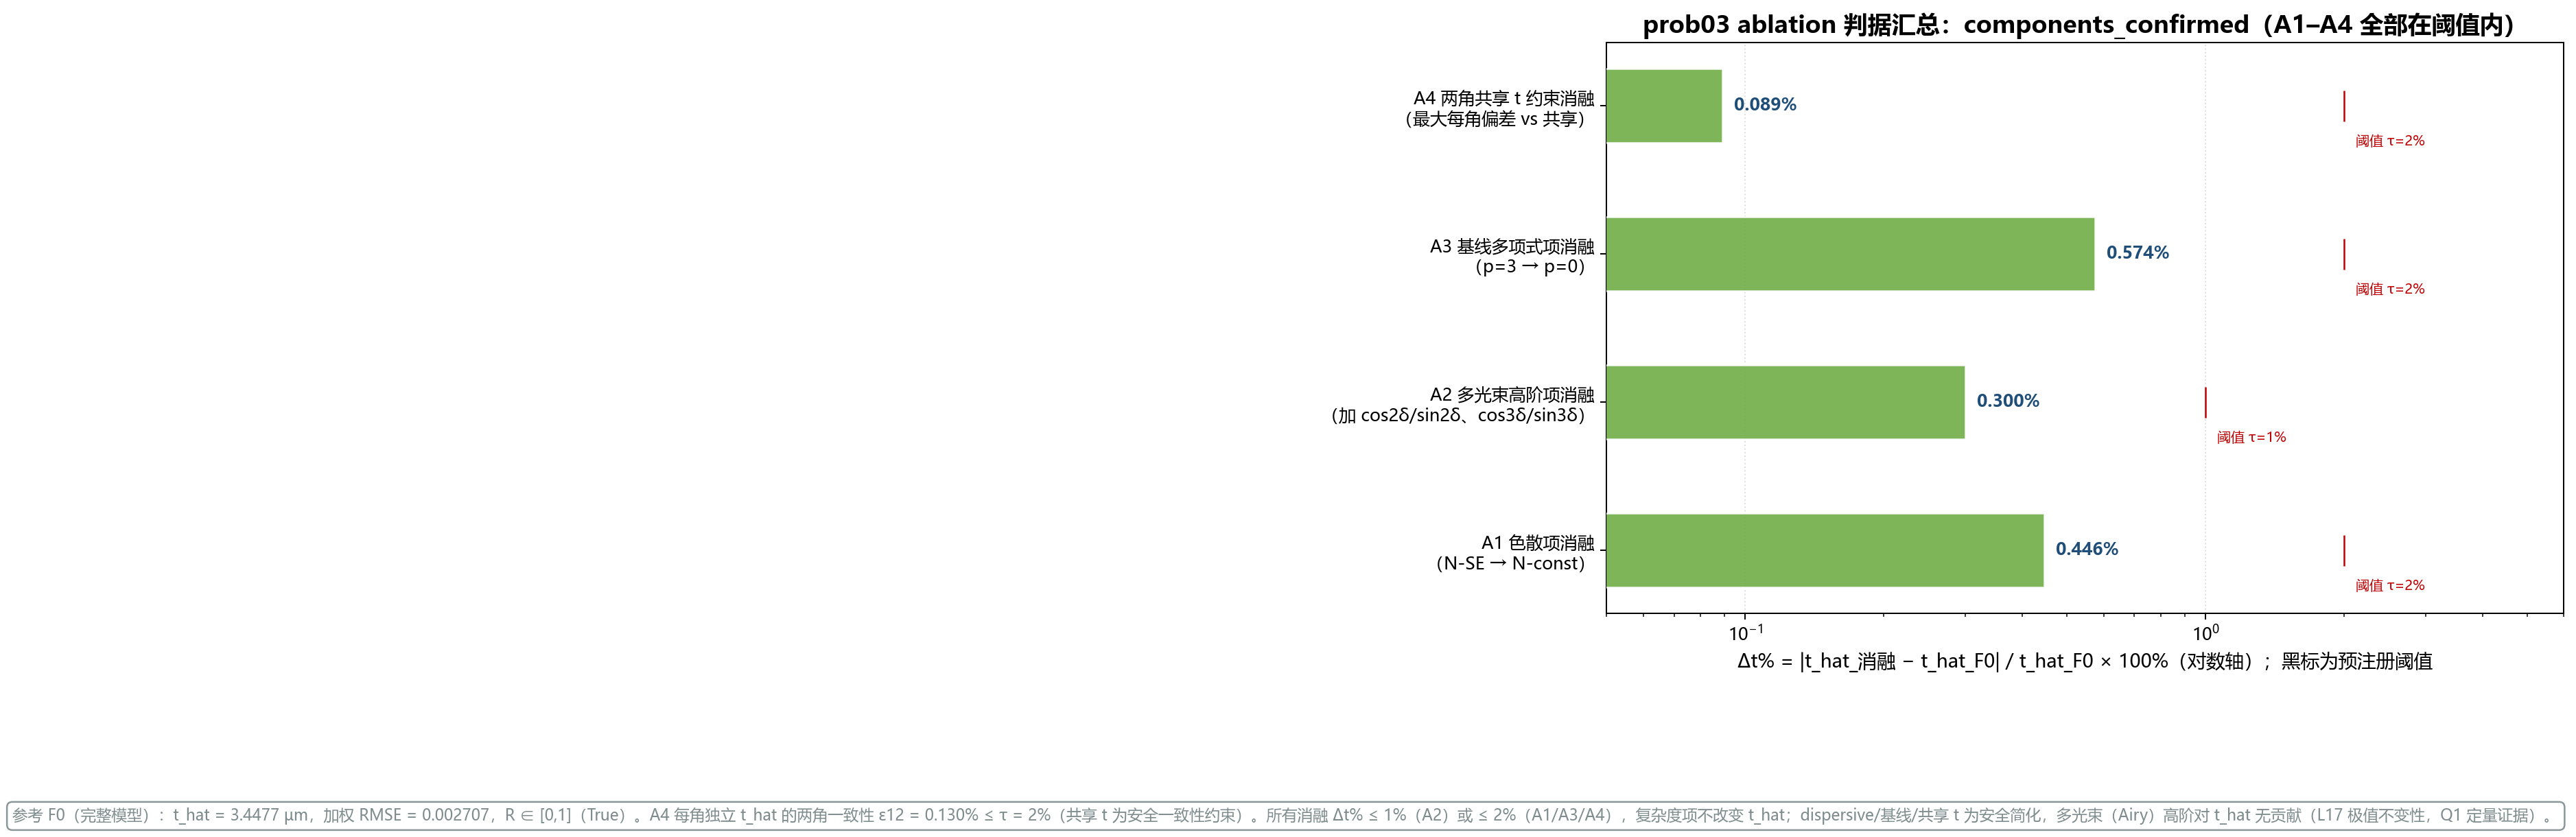
\includegraphics[keepaspectratio,alt={硅模型的消融判定汇总}]{problems/2025-cumcm-b/prob03/versions/assumption_v001/figures/prob03_fig_ablation_summary_9f93c3dd2d.png}}

硅模型的消融判定汇总

图36
汇总改变色散、加入高阶谐波、删减基线及取消共享厚度约束后的结果。各试验均按原阈值解释，不因变化小而删除不利情景。

\pandocbounded{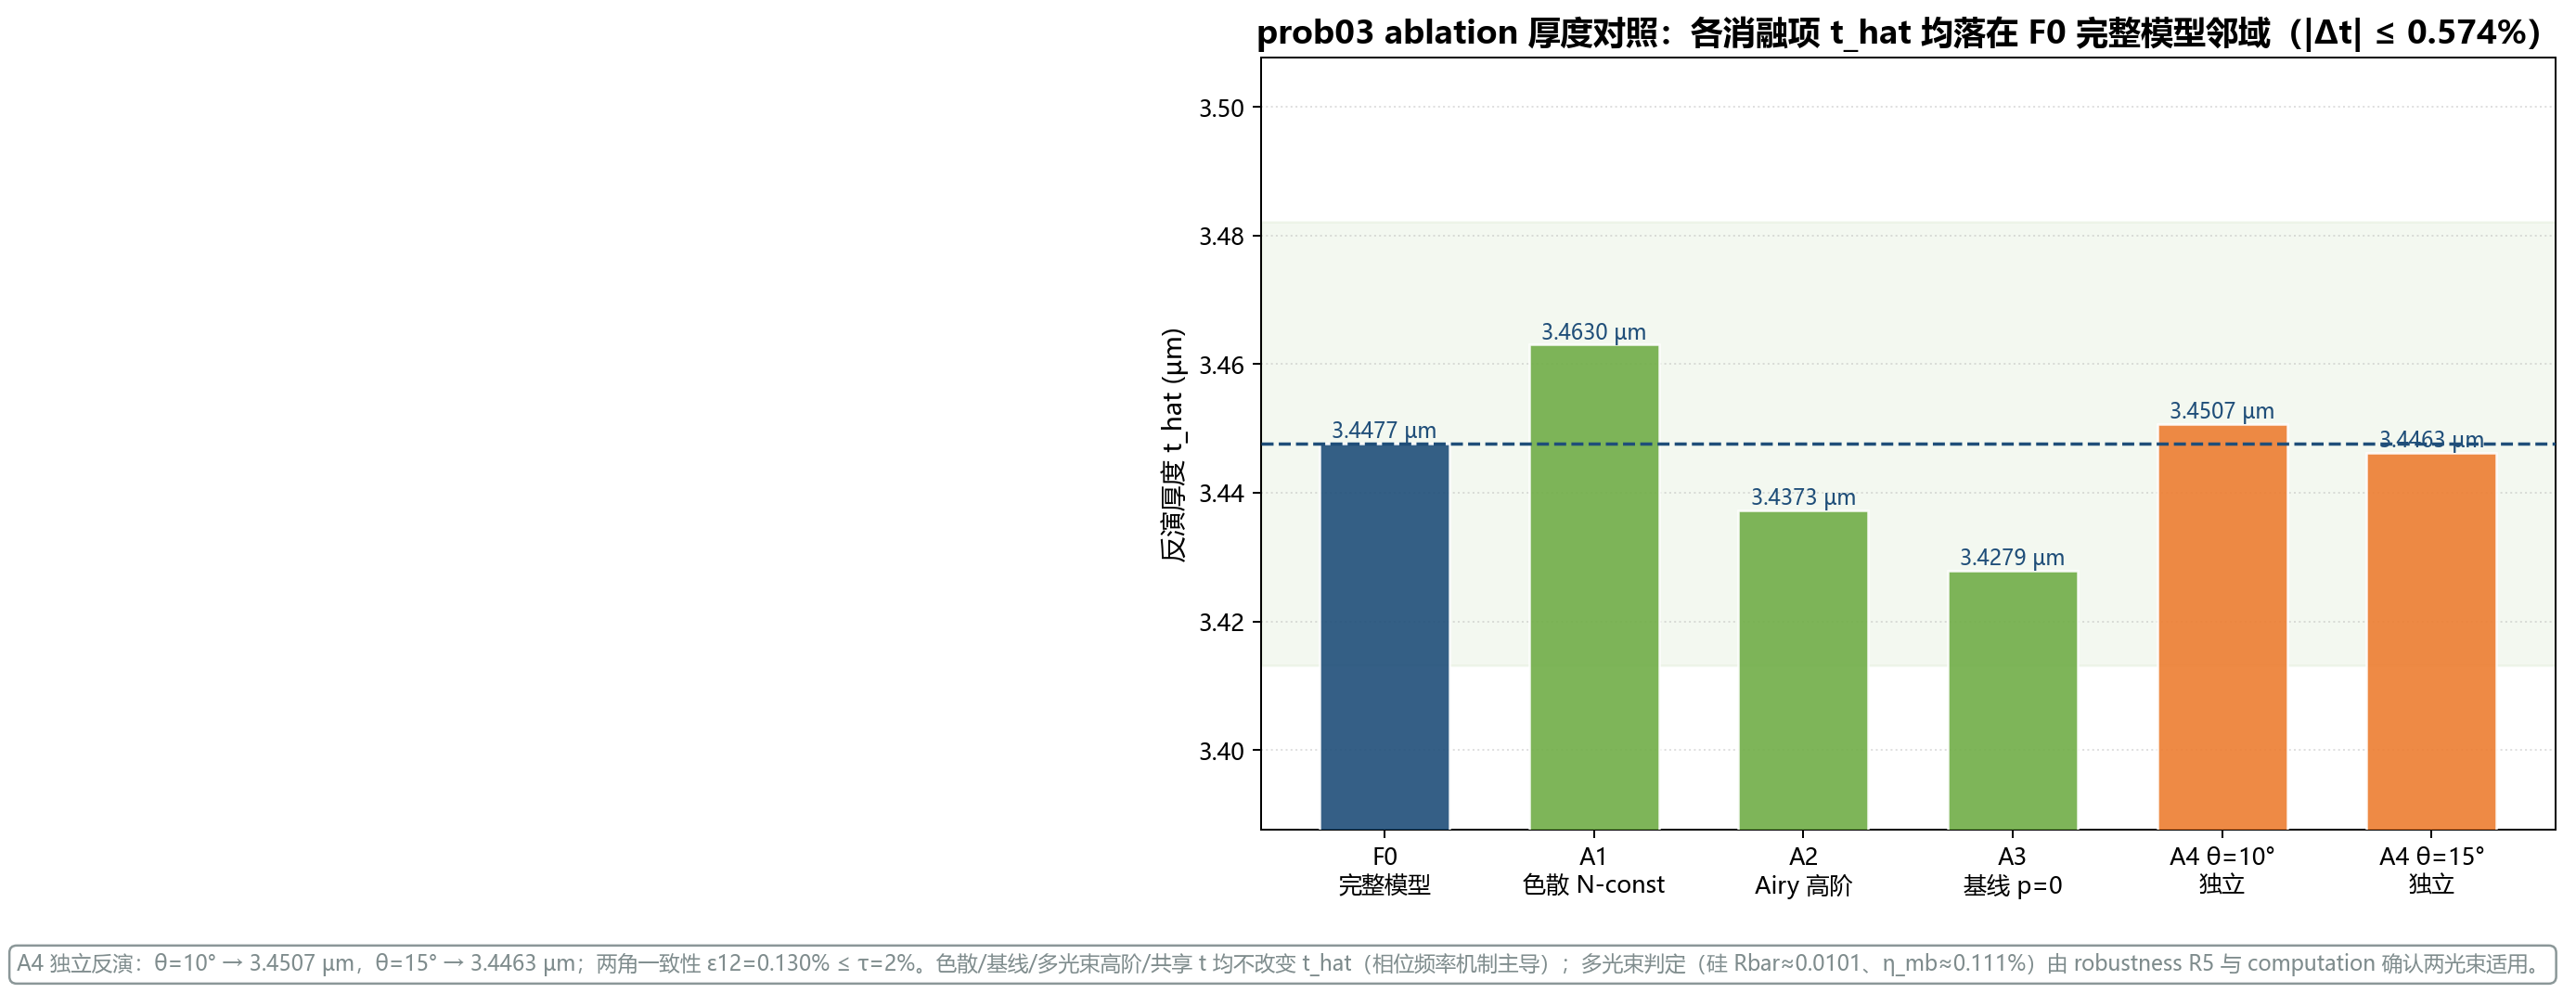
\includegraphics[keepaspectratio,alt={硅各消融方案的厚度对照}]{problems/2025-cumcm-b/prob03/versions/assumption_v001/figures/prob03_fig_ablation_t_consistency_ec44908369.png}}

硅各消融方案的厚度对照

图37
对比完整模型与各变体。加入高阶谐波后厚度变化0.300\%，表明当前数据下其影响较小，而不是有限噪声拟合中的严格零变化。

\pandocbounded{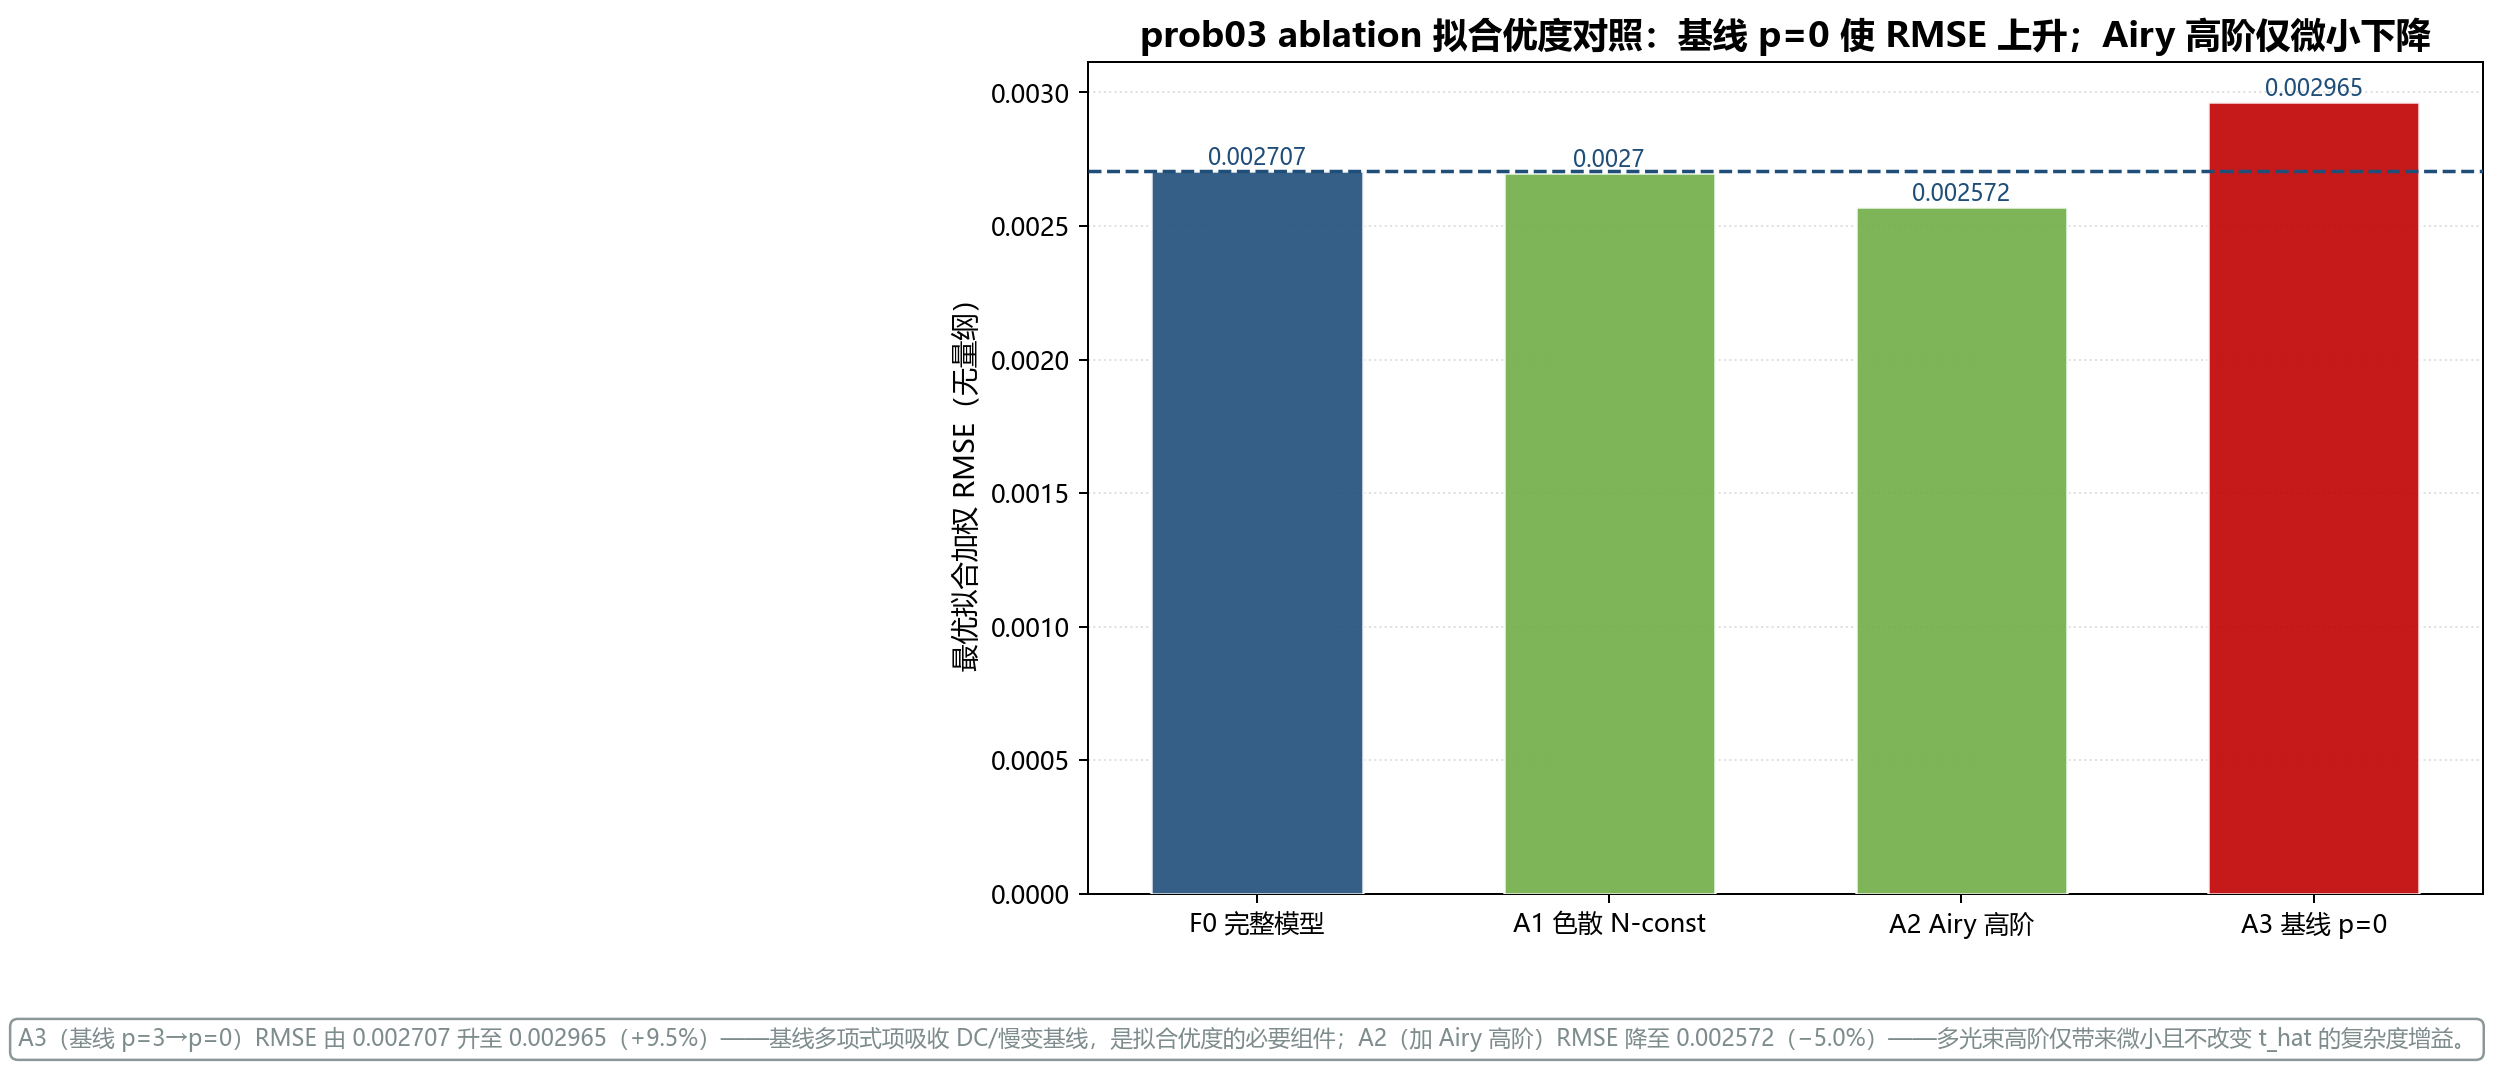
\includegraphics[keepaspectratio,alt={硅消融方案的拟合误差对照}]{problems/2025-cumcm-b/prob03/versions/assumption_v001/figures/prob03_fig_ablation_rmse_ce4b523efa.png}}

硅消融方案的拟合误差对照

图38
展示厚度稳定性与拟合优度不是同一指标。高阶谐波可改善残差，减少基线自由度则使拟合变差；不能把更低残差自动解释为更准确的厚度。

问题3 可靠性与结论

硅的色散扰动厚度变化为0.503\%，窗口敏感性为0.749\%，角度差为0.130\%。目标函数的次小候选比值约1.020，接近简并；应报告找到的最优候选及搜索条件，不应宣称具有``四倍裕度''的唯一性。约6.9
μm的倍周期候选不能与3.4477 μm主结果混淆。

主结论仍附有以下限制：衬底折射率是幅度弱辨识值；区间采用轮廓方法而非重采样；部分硅材料与多光束文献仅完成元数据或摘要层面核验；附件2存在输入清单不一致，且历史运行的部分全局配置后来发生变化，限制了严格复现的可追溯范围。窗口敏感性来自已有独立探针而非新增整套数值实验，残差比较的基线差异和周期近简并仍保留。不能以各工程阈值内的稳定性替代新的独立测量。

跨小问一致性、稳健性与消融分析

三问共享同一套相位定义和单位换算。第一问证明合成场景下相位与厚度的对应；第二问说明真实背景要求分离线性幅度参数；第三问进一步验证是否需要增加高阶反射。合成样本的10
μm不是两种实测晶圆的真值，不能将它们的厚度互相校准。

实测问题的可靠性指标对照

\begin{longtable}[]{@{}llll@{}}
\toprule\noalign{}
检查维度 & 碳化硅 & 硅 & 解释边界 \\
\midrule\noalign{}
\endhead
\bottomrule\noalign{}
\endlastfoot
两角相对差 & 0.165\% & 0.130\% & 工程一致性，不等于外部准确度 \\
色散扰动影响 & 0.507\% & 0.503\% & 限于指定材料模型与扰动 \\
95\%区间相对半宽 & 0.0911\% & 0.134\% & 条件轮廓区间，非总误差 \\
主方法对衬底折射率 & 结构解耦 & 结构解耦 & 幅度参数本身仍弱辨识 \\
高阶反射是否触发修正 & 否 & 否 & 依赖当前谱段和阈值 \\
\end{longtable}

扰动分析改变输入或模型设定，消融则移除特定组成部分，二者不能混为一谈。碳化硅删除基线会明显移动厚度，说明相位提取需要处理背景；硅高阶谐波主要改善残差而厚度变化较小，说明较复杂的模型未必带来相同比例的测厚收益。所有这些判断均限定于已有实验，不追加新的优化结果。

模型评价、局限与推广

模型的主要优点是物理量与数值参数之间的对应清楚：相位带有几何厚度，基线和包络吸收缓变背景，Airy项回答高阶反射问题。一维搜索与线性子问题便于比较周期候选，也便于解释单次局部拟合为何可能失败。

局限主要有四类。其一，材料色散和吸收条件有适用范围，超出该范围不能延长公式即视为完成验证。其二，主结果仍有背景阶数、窗口和弱可辨识引起的模型选择不确定性。其三，没有独立测厚真值，窄置信区间只反映特定模型内部的不确定性。其四，文献全文、原始输入副本及历史配置的追溯尚不完全，本文如实保留这一复现限制。

因此，推广到不同掺杂、温度、粗糙度或非平行结构时，应重新检查光学常数、吸收和仪器背景。未来可用独立测厚结果、重复测量与残差重采样评价系统误差；这些是后续验证方向，不是本论文已经执行的实验。

结论

在透明、近似平行的界面条件下，色散相位函数给出了斜入射干涉周期与厚度的统一关系。合成实验说明显式保留色散能够消除常数折射率近似的主要系统偏差，多候选比较有助于识别周期歧义。

对两角实测数据，变量投影方法给出碳化硅共享厚度7.2158
μm、硅共享厚度3.4477
μm，对应角度相对差分别为0.165\%和0.130\%。碳化硅统计检验的拒绝结果与较小工程差异并存；硅邻近周期候选接近简并。二者都要求附条件报告，不能把估计值写成无误差的材料常数。

在当前材料参数、透明谱段和预设判据下，两种晶圆均不需要显著多光束修正。相较于盲目增加模型阶数，控制色散依据、基线处理和周期候选选择更重要。论文中的图表、程序与结果来自同一批既有记录；本次写作未重新建模或计算。

参考文献

Albert, M. P., Combs, J. F.. Thickness Measurement of Epitaxial Films by
the Infrared Interference Method. Journal of The Electrochemical
Society, 1962.

Schumann, P. A.. The Infrared Interference Method of Measuring Epitaxial
Layer Thickness. Journal of The Electrochemical Society, 1969.

ASTM International. ASTM F95-89(2000): Standard Test Method for
Thickness of Lightly Doped Silicon Epitaxial Layers on Heavily Doped
Silicon Substrates Using an Infrared Dispersive Spectrophotometer. ASTM
International（标准组织正式文件）, 2000.

SEMI. SEMI MF95 (SEMI MF009500): Test Method for Thickness of Lightly
Doped Silicon Epitaxial Layers on Heavily Doped Silicon Substrates Using
an Infrared Dispersive Spectrophotometer. SEMI International Standards,
2013.

Weeks, S. P.. Thickness Measurement of Thin (1.0-µm) Epitaxial Silicon
Layers by Infrared Reflectance. Silicon Processing (ASTM STP 804), 1983.

Born, M., Wolf, E.. Principles of Optics: Electromagnetic Theory of
Propagation, Interference and Diffraction of Light (7th ed.). Cambridge
University Press（权威教材）, 1999.

Hecht, E.. Optics (5th ed., Global Edition). Pearson（权威教材）, 2017.

Shaffer, P. T. B.. Refractive Index, Dispersion, and Birefringence of
Silicon Carbide Polytypes. Applied Optics, 1971.

Wang, S., Zhan, M., Wang, G., Xuan, H., Zhang, W., Liu, C., Xu, C., Liu,
Y., Wei, Z., Chen, X.. 4H-SiC: a new nonlinear material for midinfrared
lasers. Laser \& Photonics Reviews, 2013.

Xu, C., Wang, S., Wang, G., Liang, J., Wang, S., Bai, L., Yang, J.,
Chen, X.. Temperature dependence of refractive indices for 4H- and
6H-SiC. Journal of Applied Physics, 2014.

Polyanskiy, M. N.. Refractiveindex.info database of optical constants.
Scientific Data, 2024.

Li, H. H.. Refractive index of silicon and germanium and its wavelength
and temperature derivatives. Journal of Physical and Chemical Reference
Data, 1980.

Palik, E. D. (ed.). Handbook of Optical Constants of Solids (Vol. 1-3).
Academic Press（权威手册）, 1998.

Spitzer, W., Fan, H. Y.. Infrared Absorption in n-Type Silicon. Physical
Review, 1957.

Pernot, J., Camassel, J., Peyre, H., Robert, J.-L.. From Transport
Measurements to Infrared Reflectance Spectra of n-Type Doped 4H-SiC
Layer Stacks. Materials Science Forum, 2003.

Chahal, J. S., Rahbany, N., El-Helou, Y., Wu, K.-T., Bruyant, A.,
Zgheib, C., Kazan, M.. Temperature dependence of the anisotropy of the
infrared dielectric properties and phonon-plasmon coupling in n-doped
4H-SiC. Journal of Physics and Chemistry of Solids, 2023.

王晨茜, 孙嘉妍, 陈怡佳, 杜睿.
基于色散修正与全谱拟合的红外干涉测厚模型研究.
数学建模及其应用（Mathematical Modeling and Its Applications）, 2026.

Harrick, N. J.. Determination of Refractive Index and Film Thickness
from Interference Fringes. Applied Optics, 1971.

Larruquert, J. I., Pérez-Marín, A. P., García-Cortés, S., Rodríguez-de
Marcos, L., Aznárez, J. A., Méndez, J. A.. Self-consistent optical
constants of SiC thin films. Journal of the Optical Society of America
A, 2011.

Liu, Lu, Shi, Weiwei, Xu, Shibo, Wang, Xiaofan. Dispersion Compensation
and Multi-Beam Interference Correction Algorithm for Thickness
Measurement of SiC Epitaxial Layer. Sensors, 2026.

Mainali, Madan K., Dulal, Prabin, Shrestha, Bishal, Amonette, Emily,
Shan, Ambalanath, Podraza, Nikolas J.. Optical properties of 4H-SiC and
6H-SiC from infrared to vacuum ultraviolet spectral range ellipsometry
(0.05--8.5 eV). Surface Science Spectra, 2024.

Lindquist, O. P. A., Schubert, M., Arwin, H., Järrendahl, K.. Infrared
to vacuum ultraviolet optical properties of 3C, 4H and 6H silicon
carbide measured by spectroscopic ellipsometry. Thin Solid Films, 2004.

Lindquist, O. P. A., Arwin, H., Henry, A., Järrendahl, K.. Infrared
Optical Properties of 3C, 4H and 6H Silicon Carbide. Materials Science
Forum, 2003.

Tong, Zhen, Liu, Linhua, Li, Liangsheng, Bao, Hua. Temperature-dependent
infrared optical properties of 3C-, 4H- and 6H-SiC. Physica B: Condensed
Matter, 2018.

Sunkari, Swapna, Mazzola, M. S., Mazzola, J. P., Das, Hrishikesh, Wyatt,
J. L.. Investigation of longitudinal-optical phonon-plasmon coupled
modes in SiC epitaxial film using Fourier transform infrared reflection.
Journal of Electronic Materials, 2005.

Mazzola, Michael S., Sunkari, Swapna G., Mazzola, Janice, Das,
Hrishikesh, Melnychuck, Galyna, Koshka, Yaroslav, Wyatt, Jeffery L.,
Zhang, Jie. Improved Resolution of Epitaxial Thin Film Doping Using FTIR
Reflectance Spectroscopy. Materials Science Forum, 2005.

Zhou, Zhen-Hong, Yang, Isabel, Yu, Fuzhong, Reif, Rafael. Fundamentals
of epitaxial silicon film thickness measurements using emission and
reflection Fourier transform infrared spectroscopy. Journal of Applied
Physics, 1993.

Sun, Jiaxing, Li, Zhisong, Zhang, Haojie, Song, Jinlong, Zhai, Tianbao.
An improved method for measuring epi-wafer thickness based on the
infrared interference principle: Addressing interference quality and
multiple interferences in double-layer structures. Results in Physics,
2023.

Severin, P. J.. On the Infrared Thickness Measurement of Epitaxially
Grown Silicon Layers. Applied Optics, 1970.

Sato, K., Ishikawa, Y., Sugawara, K.. Infrared interference spectra
observed in silicon epitaxial wafers. Solid-State Electronics, 1966.

Soler, F. J. P.. Multiple reflections in an approximately parallel
plate. Optics Communications, 1997.

Monzón, J. J., Sánchez-Soto, L. L., Bernabeu, E.. Influence of coating
thickness on the performance of a Fabry--Perot interferometer. Applied
Optics, 1991.

附录：复现说明、文件清单和核心代码索引

随文支撑材料包含各小问的计算与绘图代码、参数登记、运行配置和按正式图号命名的图片。运行顺序为先完成合成验证，再对碳化硅和硅数据分别执行主计算，随后使用相应结果进行扰动、消融与绘图；每次运行使用独立输出目录，不覆盖原结果。

原始竞赛附件因分发许可未确认，不随包提供，应从题目发布方合法取得并核对材料、入射角、列含义与数据版本。支撑材料运行说明列出所需输入及目录关系；其中程序接口与依赖进行了静态检查，本次没有执行全数据集复算。由此，论文交付与软件检查完成不等于已验证在另一台机器上数值完全复现。
